\cleardoublepage
\chapter{Computing standing waves}
\label{sec:chapter2}

\section{Introduction}
\label{sec:chapter2_0}

\subsection{The importance of calibrating and modeling instruments}

Microscopes, mass spectrometers, hourglasses, seismographs, measuring tape, magnetic resonance imagine scanners, telescopes, 
we build instruments to measure parameters and properties of the objects and events around us.

The more accurate the instrument, the more precisely we can constrain the value of these physical parameters.
With enough precision, we can confirm of infirm hypotheses, reinforce theories or find their limitations, and advance science.
Noise and imperfections in our instruments obviously limit the precision that we can achieve and hinder scientific progress.

There is another source of uncertainty: we do not always know well enough how our instruments behave.
Even an instrument built perfectly according to specifications, perfectly protected from exterior perturbations and maintained perfectly stable can behave in ways that we do not understand fully.
In mathematical terms, the transfer function~$F$ of an instrument often involves parameters for which the value is not well known at the moment of the observation.
\begin{equation}
    y = F(x, p_0, p_1, p_2, p_3, p_4, \dots)
\end{equation}
When we invert $F$ to retrieve the real value $x$ of the physical parameter of interest from the value $y$ that we measured, any unknown parameter $p_i$ adds to the uncertainty.
When confronted to unknown parameters, we have three possible courses of action.

The first possibility is to do nothing.
We will never know the instrument with an absolute precision.
When the uncertainty is acceptable, then we accept it and draw error bars on our plots.

The second possibility is to take measurements of well known reference sources.
Each new measurement yields a new equation, each equation allows to solve for one unknown.
This is called ``calibrating the instrument''.
The time scale upon which the instrumental parameters drift determines how often we must recalibrate it.

The third possibility is to calculate the value of these unknown parameters by modeling the physics that happens inside the instrument.
For example, how the temperature of an instrument contracts or expands its optical lenses can be computed from first principles.

Why would we ever go through the troubles of modeling parameters when we can `simply' measure them with calibration measurements?
There are many reasons.
The time spent calibrating the instrument is not spent measuring interesting things.
There may just be too many parameters.
The instrument might not even exist anymore, and we are left with an archive of data that might or might not contain the observation you need to determine the value that parameter $p_7$ had in December three years ago.

\subsection{Focus on the optics of HIFI}

This chapter describes the result of our efforts to model electromagnetic interferences in a coherent high-resolution spectrometer.
The Heterodyne Instrument for the Far Infrared (HIFI)~\cite{AA_518_L6} is a state-of-the art high-resolution spectrometer designed for the study of the chemistry and dynamics of a wide range or astrophysical environment such as star forming regions, galactic evolution and planetary atmospheres.
HIFI operates between~\num{640} and \SI{1910}{\giga\hertz}, a frequency range that is covered by seven bands.
The absolute calibration accuracy of HIFI is at least~\SI{10}{\percent}, with a goal of~\SI{3}{\percent}.
\Cref{tab:calibration_errors} summarizes the origin of the actual calibration uncertainties for the seven bands.
The sideband ratio and the optical standing waves stand out in this table for being amongst the biggest contributors to the uncertainty.

\begin{table}[hbtp]
    \centering
    \begin{tabular}{lcccc}
        \toprule
        Error source           & Band 1/2 & Band 3/4 & Band 5 & Band 6/7 \\
        \midrule
        Sideband ratio         & 3--4     & 4--6     & 4--6   & 5--8     \\
        Hot load coupling      & <1       & <1       & <1     & <1       \\
        Cold load coupling     & <1       & <1       & <1     & <1       \\
        Hot load temperature   & <1       & <1       & <1     & <1       \\
        Cold load temperature  & <1       & <1       & <1     & <1       \\
        Planetary model error  & <3       & <3       & <3     & <3       \\
        Beam Efficiency        & <5       & <5       & <10    & <5       \\
        Pointing               & <1       & <2       & <2     & <4       \\
        Optical standing waves &  4       & 4        & 3      & 3        \\
        \bottomrule
    \end{tabular}
    \caption{Overall error budget of HIFI.}
    \caption*{
        This tables provides the percentage flux error associated with each component of the error budget.
        Source: \citetitle{hifiobserversmanual}~\cite{hifiobserversmanual}.
    }
    \label{tab:calibration_errors}
\end{table}

In HIFI, the problem of the sideband ratio and that of standing waves are actually related.
Both are influenced by the optics of the instrument.
Let us explain these terms in a few words.

\subsubsection{The sideband ratio}
HIFI is a heterodyne spectrometer.
Heterodyne spectrometers are sensitive to two ranges of frequencies simultaneously.
These frequency ranges are called ``sidebands''; the sideband with the lowest frequencies is called ``lower sideband'' (LSB), and the other ``upper sideband'' (USB).
A heterodyne spectrometer overlaps these two sidebands and returns a single measurement value~$y$, as shown in~\cref{eq:explain_sbr_0}.
\begin{equation}
    y = G_\text{LSB} b_\text{LSB} + G_\text{USB} (b_\text{USB} + x)
    \label{eq:explain_sbr_0}
\end{equation}
Often, the source of interest emits radiation in one sideband only.
In our equation, we assumed that the source emits a power~$x$ in the USB.
The other sideband receives whatever background radiation~$b$ is emitted at that time.
The background radiation is usually well known, our real unknown is~$x$.
Our problem comes from the fact that the gain of the instrument in the LSB ($G_\text{LSB}$) is different from the gain in the USB ($G_\text{LSB}$).

Let us rewrite the previous equation in a way that explicitly shows the imbalance between the sidebands.
\begin{equation}
    y =
    (G_\text{LSB} + G_\text{USB})
    \bigg( (1-g) b_\text{LSB} + g (b_\text{USB} + x) \bigg)
    \label{eq:explain_sbr_1}
\end{equation}
Here, $g = G_\text{USB}/(G_\text{LSB} + G_\text{USB})$ and is called ``sideband ratio''.
The sideband ratio equals 0.5 when the detector is balanced.

It is relatively easy to calibrate the value of total gain $G_\text{LSB} + G_\text{USB}$:
just observe at a point in the sky for which $x=0$.
However, calibrating the sideband ratio~$g$ is not easy: it is actually a combination of many instrumental parameters.

There are two contributions to the sideband ratio: the mixer gain, and the coupling of the mixer to the source.
In this book, we are interested in the second contribution: the coupling of the mixer to the source.
We want to model the effect that the optics of HIFI has on its sideband ratio. 

\subsubsection{Standing waves}
Another considerable source of uncertainty in HIFI, according to~\cref{tab:calibration_errors}, is the presence of standing waves in the optics.
Standing waves refer to electromagnetic waves trapped between reflective surfaces in an instrument.
They are a result of an electromagnetic wave interfering with itself.
These interferences modulate the coupling of the mixer to the source.
They also modulate the coupling of the mixer to the sources that are used for calibration, but they do it differently, so they cannot be calibrated out.
Here as well, modeling the optics should predict the loss of coupling due to interferences.

\subsubsection{Coherence}
The channels of HIFI have a bandwidth of~\SI{1.1}{\mega\hertz} or lower.
When the bandwidth is so narrow, the thermal noise of the astronomical source, the calibration black bodies and the local oscillator (LO) qualify as ``narrow band Gaussian noise signals''~\cite{siegman1986lasers}.
They have a coherence time~$\tau$ equal to the inverse of their bandwidth~$\tau=1/\Delta f$.
A bandwidth of~\SI{1}{\mega\hertz} results in a coherence time of~\SI{1}{\micro\second} equivalent to a coherence length of~\SI{300}{\meter}.
This is a hundred times the longest distance inside HIFI.
Therefore, in HIFI, the signals from the LO, the calibration sources and the sky are coherent.

The notion of coherence refers to the degree of correlation, described in a specific mathematical fashion, between two signals observed at different points in time and/or space.
The amplitude, the phase and the polarization of the electromagnetic waves inside HIFI change only slowly with time.
The amplitude, phase and polarization of the wave at any one time is strongly correlated with the amplitude phase and polarization of that same wave at considerably earlier or later times.
Between these two moments, the wave may have undergone several reflections on the various optical elements that make the instrument.
These reflections can make the wave overlap itself in space, and the strong degree of phase correlation implies that the wave interferes with itself.

Reflections in a coherent system give rise to interferences, and interferences inside a cavity create standing waves.
Any two surfaces that face each other via at least one optical path form a cavity.
The cavity formed by the detector and the secondary mirror is one that is often considered during the design of a telescope.
Other cavities exist inside HIFI: the mixers, local oscillators, calibration loads, diplexer roof-top mirrors, beam splitters, are all surfaces that somehow face each others.

In his technical note from~\citedate{whyborn2002standingwaves} entitled
\citetitle{whyborn2002standingwaves},
\citeauthor{whyborn2002standingwaves} mentions that standing waves can not only modulate the optical coupling between a source and a detector (as we will spend the rest of this chapter exploring), but also the intrinsic noise of the mixer itself.
We are not going to cover that second point.
In this chapter, we focus on modeling the interferences in the optical path.

\subsection{Why a new technique?}
Because the far-infrared is between the microwave and optical domains of the electromagnetic spectrum, many modeling techniques developed for microwave or optical engineering can be applied to the far-infrared.
However, no technique exists that can deal with both the optical and the microwave aspect at the same time.

From the optical side, we can use ray tracing~\cite{spencer1962general}.
Ray tracing often assumes that the light is incoherent and propagates along infinitely-thin beams.
Laser theory introduces some tools to deal with coherence and the self-diffraction of the beam~\cite{siegman1986lasers}.
These theories make use of matrices to describe changes to the degree of polarization of light (Stokes parameters, Müller matrices, Jones matrices), and to the geometry of the beam (ray optics or Gaussian beams ABCD matrices)~\cite{goldsmith1998quasioptical}.

From microwave circuits and waveguides theory, we can use the many types of 2--by--2 matrices that link voltage and current for two-ports networks: there is a homomorphism between \{voltage, current, relations between them\} and \{electric field, magnetizing field, relations between them\}.
There are also scattering matrices which allow for more than two ports~\cite{pozar2009microwave}.

\Cref{tab:tools} presents a brief overview of different tools used to model optical or microwave systems.
We will not describe them all.
Suffice to say that there is no magic bullet that treats all the aspect of the problem at once.
Some tools are designed explicitly to model polarization for example, others can be tweaked in order to include it, and other tools again are just not made for that.

In this chapter, we are not proposing a such magic bullet.
We are going to combine several techniques inspired from circuit theory (notably scattering and Jones matrices), extend them to work in three dimensions, and show how to solve the steady state of optical systems of any size and complexity.
For now, we are ignoring the geometry of the beam: we assume that our waves are plane and our signals are mono-modes.
This is a first-order approximation that lets us focus on the intensity, phase and polarization coherence of these waves.

\begin{sidewaystable}[hbtp]
    \centering
    {\footnotesize
    \rowcolors{1}{gray!20}{}
    \begin{tabularx}{\textwidth}{X|X X X X X X}
        \toprule
                                          & Ray tracing & Ray optics ABCD matrix & 2-port network matrices & Scattering matrix & Jones matrix & Müller matrix  \\
        \midrule
        Intensity/power                   & yes         & no                     & yes                     & yes               & yes          & yes            \\
        Phase (coherence)                 & yes         & yes                    & yes                     & yes               & yes          & no             \\
        Polarized                         & yes         & possible               & irrelevant              & possible          & yes          & yes            \\
        Unpolarized                       & yes         & yes                    & irrelevant              & possible          & no           & yes            \\
        Direction of propagation          & yes         & a bit                  & no                      & no                & no           & no             \\
        Gaussian beam width and curvature & no          & yes                    & no                      & no                & no           & no             \\
        Gaussian beam modes               & no          & yes                    & no                      & no                & no           & no             \\
        More than 2 ports                 & yes         & no                     & no                      & yes               & no           & no             \\
        Cascade-able                      & yes         & yes                    & some                    & no                & yes          & yes            \\
        Steady-state                      & no          & no                     & yes                     & yes               & no           & no             \\
        \bottomrule
        \end{tabularx}
    }
    \rowcolors{1}{}{}
    \caption{\label{tab:tools}No tool or framework satisfies all the criteria.}
\end{sidewaystable}
    
\subsection{Our goal}

We wish to model the interferences in a heterodyne instrument in order to determine more accurately the transmission efficiencies between various sources of radiation and the detector.

Why replace unknown optical efficiency parameters with unknown model parameters?
Because this reduces considerably the number of parameters.
Instead of having one ad-hoc totally unknown mixer--LO efficiency per frequency channel (there are 8192 such channels in a HIFI spectra), the model that we propose predicts them all from a few dozen physical parameters for which we can make very educated guesses or accurate lab measurements (reflection coefficients, distances).

No model is perfect: models rely on simplifications, and their predictions within these specifications can only be as accurate as our knowledge of the model parameters.

In the best case scenario, we will manage to figure out all the physical parameters of HIFI, allowing us to recalibrate the entire data archive of HIFI to cancel the effect of interferences.
Naturally, this best case scenario is somewhat ambitious: obtaining a perfect quantitative match between the model and the data is a difficult task.

More realistically, the model that we propose could become very helpful to the engineers who are designing instruments.
Our technique can give useful qualitative predictions, even when the parameters of the models are nothing but educated guesses (more on this in~\cref{sec:chapter3})
Like good software developers do not optimize their code until profiling indicates which routines are bottlenecks, good engineers do not spend resources trying to reduce interferences unless they know which ones matter and where they occur.

\subsection{Layout of the chapter}

This chapter is divided into four sections.

\Cref{sec:chapter2_1}, \textit{\nameref{sec:chapter2_1}}, describes the concepts of electromagnetism that we use throughout the chapter.
It includes a list of the simplifications and assumptions that we make.

\Cref{sec:chapter2_2}, \textit{\nameref{sec:chapter2_2}}, explains how a cavity works, how it modulates the coupling of the detector to the source, where the lost energy goes, how it depends on frequency and how it produces ripples on spectra.

\Cref{sec:chapter2_3}, \textit{\nameref{sec:chapter2_3}}, presents the method that we have developed to calculate the coupling between any two points of a coherent instrument.
We first detail the mathematics, keeping things theoretical.
Then we propose a way to concretely implement the theory, by providing algorithms illustrated with examples.
This solver does not take an iterative approach to deal with infinite reflections, instead it solves directly for the steady state.

\Cref{sec:chapter2_4}, \textit{\nameref{sec:chapter2_4}}, is a catalog of models of various optical elements: distances, beam splitters, wire grid polarizers, mirrors.
We explain how to create matrices for each of these elements in a format that is compatible with the expectations of the solver presented in~\cref{sec:chapter2_3}.

%#############################################################################

\section{Mathematical description of plane waves}
\sectionmark{Mathematical description of plane waves}
\label{sec:chapter2_1}

%=============================================================================

\subsection{Simplifications}

As we briefly mentioned in our introduction, the modeling technique that we present in this chapter ignores self-diffraction of the electromagnetic beam
(see \citetitle{goldsmith1998quasioptical} by \citeauthor{goldsmith1998quasioptical}~\cite{goldsmith1998quasioptical} for a detailed explanation of Gaussian beams and their modes).
The model that we propose works with plane waves.

We are working toward a zero-order description of the system that includes the complicated interactions between all the cavities via all the possible optical paths, rather than considering the higher-order effects related to the spatial distribution of the reflected fields and exchange/scattering of power between modes.

One justification for this simplification is that HIFI has well-designed and matched optics, so that the dominant reflections in the system always reflect power back in roughly the same beam mode.
In particular, HIFI makes use of corrugated horns to couple the optical beams to the local oscillator diodes or the mixers.
When corrugated horns are used with properly tuned waveguides, they emit and receive single-mode beams (see~\citetitle{clarricoats1966propagation} by \citeauthor{clarricoats1966propagation}~\cite{clarricoats1966propagation}).
Similarly, a device designer makes sure that his microwave circuit will optimally couple to the fundamental waveguide mode by selection of coupling structures, the device substrate, in general by impedance matching to the electromagnetic environment (embedding impedance).
In other words, if any energy is converted to a high-order mode by the optics, then it will not couple to the mixer and can, for any practical purpose, be modeled with a simple term of loss.

Another justification for the validity of our plane-wave approach is that most of the optical elements of HIFI are placed at the waist of the beams, where the wavefront is plane.

%=============================================================================
\subsection{Conventions and definitions}
Plane waves are solutions to Maxwell's equations~\cite{hecht2002optics}, which describe the electro-magnetic field in time and space.
Although plane waves cannot physically exist (their wavefront is an infinite plane, carrying an infinite energy), they are often very good approximations to many problems, in the same way we can ignore the curvature of the Earth to build a house.

Equations \eqref{eq:e_r_t_real_minus} and \eqref{eq:e_r_t_real_plus} are two equivalent expressions of the amplitude of the electric field of a plane wave propagating along a direction~$\vect{k}$ (bold letters denote vectors).
These two expressions are equivalent because the cosine function is even.
Choosing one or the other is a matter of convention.
\begin{subequations}
    \begin{align}
       E(\vect{r}, t) &= E_0 \cos(\phantom{-}\vect{k}\cdot \vect{r} - \omega t + \varphi)   \label{eq:e_r_t_real_minus} \\
       E(\vect{r}, t) &= E_0 \cos(-          \vect{k}\cdot \vect{r} + \omega t - \varphi)   \label{eq:e_r_t_real_plus}
    \end{align}
    \label{eq:e_r_t_real}
\end{subequations}
In \cref{eq:e_r_t_real}, $t$ is the time coordinate and~$\vect{r}=(x, y, z)$ the space coordinates.
$\varphi$ is related to initial conditions and the choice of reference frame.
$E_0$ is the amplitude of the electric field.
It has the dimension of an electric potential per unit length.
It is given for example in volts per meter or newtons per coulomb.

\Cref{eq:e_r_t_real} is illustrated \cref{fig:plane_wave_propagation} as a function of~$z$ for a few values of~$t$, assuming a propagation of direction that has a non-zero $z$ component.

\begin{figure}[hbtp]
    \centering
    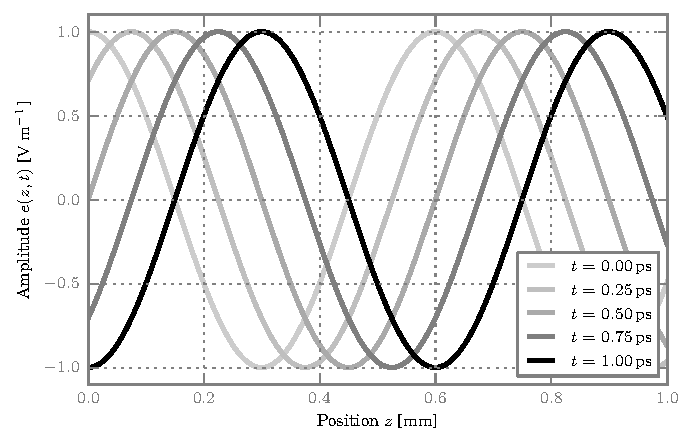
\includegraphics{plane_wave_propagation}
    \caption{Electric field amplitude of a wave of frequency \SI{500}{\giga\hertz} and amplitude \SI{1}{\volt\per\meter} propagating in vacuum (refractive index 1).}
    \label{fig:plane_wave_propagation}
\end{figure}


\begin{table}[hbtp]
    \centering
    \caption{Notations and definitions of electromagnetic constants and parameters}
    \caption*{
        All the entries in this table are real numbers.
        
        The values and definitions listed in this table assume the current (early 2014) SI base units.
        A proposal will be discussed during the
        25\textsuperscript{th} meeting of the Conférence Générale des Poids et Mesures on 18-20 November 2014:
        \citetitle{mills2006redefinition} by~\citeauthor{mills2006redefinition}~\cite{mills2006redefinition}.
        Under this proposal, the definition of the Ampere undergoes a major redefinition and
        becomes an exact number of Coulomb per second, with the Coulomb being exact as well:
        the charge of the electron is not measured anymore but fixed.
        As a result, $\mu_0$ is not exact anymore but becomes a measured value.
        This table is correct until the proposal for redefinition of the SI units is accepted.
    }
    \label{tab:definitions_simple}
    \rowcolors{2}{gray!25}{white}
    \begin{tabularx}{\textwidth}{l l X}
        \toprule
        \hiderowcolors
        symbol & definition & name \\
        \showrowcolors
        \midrule
        $\omega$      &  $2 \pi f$   &  angular frequency \\
        $k$           &  $2 \pi / \lambda$   &   wave number\\
        $\lambda$     &  $c / f$  &  wavelength \\
        $c$           &  $c_0 / n$  &  phase velocity \\
        $c_0$         &  $\equaldef \SI{299792458}{\meter\per\second}$  &  speed of light in vacuum \\
        $n$           &  $\sqrt{\epsilon_r \mu_r}$  &  refractive index \\
        $\epsilon_r$  &  $\epsilon / \epsilon_0$  &  relative permittivity\\
        $\mu_r$       &  $\mu / \mu_0$  &  relative permeability\\
        $\epsilon$    & measured material property & absolute permittivity \\
        $\mu$         & measured material property & absolute permeability \\
%        $\epsilon_0$  & $\approx \SI{8.854187817e-12}{\farad\per\meter}$  &  absolute permittivity of vacuum \\
        $\epsilon_0$  & $c_0^2=\dfrac{1}{\epsilon_0 \mu_0}$  &  absolute permittivity of vacuum \\
        $\mu_0$       & $\equaldef 4\pi\times 10^{-7}\>\si{\henry\per\meter}$  &  absolute permeability of vacuum \\
        $\eta$        & $\sqrt{\mu / \epsilon}$  &  intrinsic impedance\\
        $\eta_0$      & $\sqrt{\mu_0 / \epsilon_0}$  &  intrinsic impedance of free space \\
        $Z$           & $E / H$  & wave impedance \\
        $Y$           & $H / E$  & wave admittance \\
        $E$           &          & electric field amplitude \\
        $H$           &          & magnetizing field amplitude \\
        \bottomrule
    \end{tabularx}
\end{table}

As its name indicates, an electromagnetic wave does not only have an electric field, it also has a magnetic (or magnetizing) field.
However, the electric and magnetic fields are tightly coupled, and often describing one of them is sufficient when the context is known.
\Cref{tab:definitions_simple} summarizes the relations between various parameters used to describe a wave and its propagation medium.
For plane waves in homogeneous materials, $Z=\eta$.

We should note that all the parameters in this table are scalars, there are no higher-order tensors.
This means that we are not considering anisotropic propagation media yet.
This is not a fundamental limitation of our model, which could deal with anisotropy and birefringence if someone were to write scattering matrices for these cases.

All the parameters introduced in this table are real.
It is possible to add more parameters, such as the electric conductivity of a material.
Such parameters account for attenuation, phase delays, etc.
However, it is easier to deal with them by with when using complex numbers without changing any of these equations.
In \cref{sec:polar_complex_notation}, we will go over these parameters again and explore the effects of giving them an imaginary part.



%=============================================================================

\subsection{Polar complex notation}
\label{sec:polar_complex_notation}

Euler's formula, given in \cref{eq:euler_formula}, relates the trigonometric function cosine to a complex exponential.
\begin{equation}    
    \exp(i\theta) = \cos(\theta) + i\sin(\theta) \label{eq:euler_formula}
\end{equation}
In \cref{eq:euler_formula}, $i$ represents the imaginary unit such that $i^2=-1$.
If we rewrite the expression of~$E$ given in \cref{eq:e_z_t_real_minus} as a complex in polar coordinates, we have \cref{eq:e_z_t_complex_minus}.
\begin{align}
   \hat{E}(z, t) &= E_0 \exp(i(kz - \omega t + \varphi))
   \label{eq:e_z_t_complex_minus}
   \\
   E(z, t) &= \Re(\hat{E}(z, t))
   \label{eq:e_z_t_real_complex_minus}
\end{align}
The hat above the $E$ signals that $\hat{E}$ is the complex equivalent of $E$.
As shown by \cref{eq:e_z_t_real_complex_minus}, $E$ and $\hat{E}$ do not have the same value (one is real, the other is complex);
however, both describe the same physical phenomenon.

If we open the door to complex numbers, we may want to consider the effect of giving an imaginary part to the parameters of \cref{tab:definitions_simple}.

The imaginary part of the complex angular frequency $\hat{\omega} = \omega' + i \omega''$ corresponds to an amplification of the wave in time, see \cref{eq:complex_angular_frequency}.
If the imaginary part is negative, then the effect is an attenuation of the signal as time goes.
\begin{subequations}
    \begin{align}
       \hat{E}(z, t) &=
       E_0 \exp(i(kz - \hat{\omega} t + \varphi))
       \\
       &=
       E_0 \exp(i(kz - (\omega' + i \omega'') t + \varphi))
       \\
       &=
       E_0 \exp(i(kz - \omega' t + \varphi)) \exp(\omega'' t)
    \end{align}
    \label{eq:complex_angular_frequency}
\end{subequations}
This can be used to model systems that vary in time.
Since the systems we study in this book are time-invariant, $\omega$ will always be real for us.

Following the same reasoning, the imaginary part of the wavenumber $\hat{k} = k' + i k''$ corresponds to a spatial attenuation or amplification.
See \cref{eq:complex_wavenumber}.
If $k''> 0$, then the wave is attenuated as it propagates.
This can model losses in a material.
\begin{subequations}
    \begin{align}
       \hat{E}(z, t) &=
       E_0 \exp(i(\hat{k}z - \omega t + \varphi))
       \\
       &=
       E_0 \exp(i((k' + i k'')z - \omega t + \varphi))
       \\
       &=
       E_0 \exp(i(k' z - \omega t + \varphi)) \exp(-k'' z)
    \end{align}
    \label{eq:complex_wavenumber}
\end{subequations}
Having $k'' \ne 0$ gives an imaginary part to the wavelength and the phase velocity
(see \cref{tab:definitions_simple}).
All these imaginary parts mean the same thing:
the wave is getting amplified or attenuated.
However, the speed of light in vacuum is known to be a real number.
Therefore, the imaginary part of $\hat{k}$ comes from an imaginary part of the complex refractive index $\hat{n}$.
This links the attenuation of the wave to a property of the material.
Since the refractive index is derived from the relative electric permittivity and the relative magnetic permeability of a materials
($\hat{n}=\sqrt{\hat{\epsilon}\hat{\mu}}$),
any of them can be responsible for the attenuation of the wave.
Note that it is possible for the refractive index to be real even if the permittivity and the permeability have a complex part.

In many cases (vacuum, mylar, aluminum), the relative magnetic permeability is very close to 1, making the electric permittivity the only parameter able to bear an imaginary part.
This means that, in these cases, the wave is absorbed by a material because of its conductive nature.
\begin{equation}
    \hat{\sigma} = \sigma' + i \sigma''
    \label{eq:admittivity}
\end{equation}
In~\cref{eq:admittivity}, $\hat{\sigma}$, $\sigma'$ and $\sigma''$
are called ``admittivity'', ``conductivity'' and ``susceptivity''.
Their SI unit is the Siemens per meter (\si{\siemens\per\meter}).
The admittivity $\hat{\sigma}$ and the imaginary part of the permittivity $\epsilon''$ are bound by \cref{eq:epsilon_second_sigma}.
\begin{equation}   
    \epsilon'' = \hat{\sigma} / \omega
    \label{eq:epsilon_second_sigma}
\end{equation}
The higher the frequency, the less effect the admittivity has.
This is understandable as inertia and other forces prevents the electrons from moving fast enough to cancel the electric field.
The term ``conductivity'' is often used in place of ``admittivity'' when the admittivity is real.
The susceptivity contributes to the real part of the permittivity~$\epsilon$, with a dependence on~$\omega$.
\begin{equation}
    \hat{\epsilon} = \epsilon' - \frac{\sigma''}{\omega} + i \frac{\sigma'}{\omega}
    \label{eq:epsilon_admittivity}
\end{equation}

In some cases, the relative magnetic permeability $\hat{\mu}$ is very different from~1 and is able to go up to several thousands in the case of very pure iron.
It can a priori be complex.
\citeauthor{bowler2006frequency} has shown in \citetitle{bowler2006frequency} \cite{bowler2006frequency} how both the real and imaginary part of the conductivity can depend on the frequency.


Finally, the complex intrinsic impedance derived from the complex permittivity and permeability imply that the electric and magnetizing fields are not in phase.
Indeed, for a plane wave in a homogeneous material, the wave impedance $\hat{Z}=\hat{E}/\hat{H}$ equals the intrinsic impedance $\hat{\eta}=\sqrt{\hat{\mu}/\hat{\epsilon}}$.
Therefore, the imaginary part of $\hat{\mu}$ or $\hat{\epsilon}$ creates a phase difference between $\hat{E}$ and $\hat{H}$.


%=============================================================================
\subsection{Phasors}
\label{sec:phasors}
\index{phasor}
In physics and engineering, a phasor is a complex number representing a sinusoidal function whose amplitude, frequency, and phase are time-invariant.
The word ``phasor'' is a portmanteau of ``phase vector''.
Phasors separate the dependencies on the amplitude, frequency and phase into three independent factors.
This can be particularly useful because the frequency factor (which includes the time-dependence of the sinusoid) is often common to all the components of a linear combination of sinusoids.
In those situations, phasors allow this common feature to be factored out, leaving just the amplitude and phase features.
The result is that trigonometry reduces to algebra.


%-----------------------------------------------------------------------------

\subsubsection{Introducing phasors}
By applying the exponentiation identity \eqref{eq:exponentiation_identity},
\cref{eq:e_z_t_complex_minus} can also be written as \cref{eq:e_z_t_complex_factorized}.
\begin{equation}
    \exp(a+b) = \exp(a) \exp(b)
    \label{eq:exponentiation_identity}
\end{equation}
\begin{equation}
    \hat{E}(z, t)
    =
    E_0 \exp(ikz) \exp(-i\omega t) \exp({i \varphi})
    \label{eq:e_z_t_complex_factorized}
\end{equation}
In \cref{eq:e_z_t_complex_factorized}, the expression of the wave is separated into four independent factors.
This is possible because the amplitude $E_0$, the wavenumber $k$, the angular frequency $\omega$ and the phase $\varphi$ are time-invariant.
The time-invariance of $\omega$ and $k$ is guaranteed by the linearity hypothesis, while that of $E_0$ and $\varphi$ is guaranteed by the coherency hypothesis.

The time factor $\exp({-i \omega t})$ is common to all the waves present in the system.
Because of that, we can factor it out as shown in equations~\ref{eq:factor_time_out} and \ref{eq:phasor}.
In these equations, $\hat{E}(z)$ is a ``phasor representation'' of the sinusoidal function $E(z, t)$, with the time factored out and considered implicit.
\begin{align}
    \hat{E}(z, t) &= \hat{E}(z) \exp(-i\omega t) \label{eq:factor_time_out}
    \\
    \hat{E}(z) &= E_0 \exp(i(kz+\varphi)) \label{eq:phasor}
\end{align}

$\hat{E}(z)$ can be visualized as a vector on the complex plane, and $\hat{E}(z, t)$ makes that vector rotate with time.

%-----------------------------------------------------------------------------

\subsubsection{Convention}
We have shown with equations~\ref{eq:e_z_t_real_minus} and \ref{eq:e_z_t_real_plus} that there are two conventions for representing the same physical phenomenon.
Either the space factor or the time factor takes a negative sign, and that decision is a priori arbitrary.
The choice of convention influences the definition of our phasors.
We have to choose between
\cref{eq:phasor_minus} and \cref{eq:phasor_plus}.
\begin{subequations}
    \begin{align}
        \text{Either }
        \hat{E}(z) &= E_0 \exp(i(\phantom{-}kz+\varphi))
        \label{eq:phasor_minus}
        \\
        \text{or }
        \hat{E}(z) &= E_0 \exp(i(-kz-\varphi))
        \text{.}
         \label{eq:phasor_plus}
    \end{align}    
\end{subequations}

In the rest of this book, we will use the convention given in \cref{eq:phasor_minus}.
This will minimize the number of negative sign in our equations.
The negative sign is factored out in the time-factor $\exp(-i \omega t)$, which we will keep implicit most of the time.



%-----------------------------------------------------------------------------

\subsubsection{Discrete space}
In our optical systems, we are hardly ever interested in the value of the phasor at any point.
For example, when modeling the effect of a dielectric interface on a wave, we need only to know the value of the phasor at the location of the interface.
If there are two interfaces, then there are two points of interest.
This means that we do not keep the explicit dependency on $z$ in our computations but work with discrete values of $z$ as illustrated by \cref{eq:phasor_no_z}.
\begin{equation}
    \begin{aligned}
        \hat{E}_0 &= E_0 \exp(i(k_0 z_0 + \varphi_0))
        \\
        \hat{E}_1 &= E_1 \exp(i(k_1 z_1 + \varphi_1))
    \end{aligned}
    \label{eq:phasor_no_z}
\end{equation}
In \cref{eq:phasor_no_z}, the phasors $\hat{E}_n$ do not depend on a space coordinate because they are defined for a specific location.
This is the type of phasors that we will be using in the rest of this chapter.



%-----------------------------------------------------------------------------

\subsubsection{Phasor algebra}
Phasors can be added together to produce a new phasor.
That is because the sum of sinusoids with the same frequency is also a sinusoid with that frequency.
We model interferences by adding phasors.

A phasor can be multiplied by a scalar to produce a new phasor.
The scalar can be a complex number, but that does not make this scalar a phasor. 
The modulus of the scalar models the gain or absorption, while its argument models the phase shift.
That means its only effect is to change the amplitude and phase of the underlying sinusoid.
The scalar multiplication models the effect of a linear optical element on a wave.

Phasors cannot be multiplied together because electric fields do not multiply.
In algebraic terms, phasors form a vector space, not a ring.
The product of two phasors would represent the product of two sinusoids which is a non-linear operation that introduce new frequencies.
Since phasors can represent systems with one frequency only, the result of multiplying two phasors is not a phasor.
This means that computing the power transported by a wave is more subtle than just squaring the phasor, which we will study in \vref{sec:jones_vectors_and_power}.





%#############################################################################



\section{From cavity to ripple}
\label{sec:chapter2_2}

Some spectra taken with HIFI show ripples on their baseline, as shown in~\cref{fig:mars_50010cb7_WBSH_USB_chp2}.
We will show in this section how cavities in the optical path of a coherent instrument can produce such ripples.
In this section, we imagine that between our detector and the source, we have a single cavity.
\begin{figure}[htbp]
    \centering
    \includegraphics[width=.8\textwidth]{mars_50010cb7_WBSH_USB}
    \caption{Continuum and absorption line of Mars with ripples.}
    \caption*{
        HIFI spectrum taken from the observation ID 0x50010cb7.
        The baseline of this spectrum, which corresponds to the continuum emission of the planet, should be flat.
        Its periodic modulation indicates the presence of cavities in the optical system, the effect of which was not calibrated out.
    }
    \label{fig:mars_50010cb7_WBSH_USB_chp2}
\end{figure}

%=============================================================================

\subsection{Reflection and transmission efficiency}

\begin{figure}[hbtp]
    \centering
    \input{cavity.pdf_tex}
    \caption{Cavity, notations.}
    \caption*{
       The vertical dotted lines represent the surfaces delimiting the cavity.
       The dotted arrows $a$ and $b$ are phasors;
       $a$ is a phasor incident to a surface and
       $b$ a phasor going away from it.
       The solid arrows represent coefficients of reflection, transmission and propagation.
       $r$ is a coefficient of reflection.
       $t$ is a coefficient of transmission.
       $s$ is the effect of propagating in space between the two surfaces.
       All these parameters are complex.
    }
    \label{fig:cavity_notations}
\end{figure}

Two reflective surfaces facing each other form a cavity.
When these surfaces are parallel to each other, we speak of Fabry-Pérot\index{Fabry-Pérot} cavity.
In this section, we will explore a Fabry-Pérot cavity.
The results are applicable to other cavities.


Each surface has two sides, so we have four sides in total that we label with the number 1 to 4 as illustrated on~\cref{fig:cavity_notations}.
Let us consider the general case in which the reflection and transmission coefficients differ for each side of each surface,
which happens in practice when the three regions of space separated by the two surfaces have different refractive indices.
We note the incident electric field phasor $a_1$, this is the signal from the source.
We are interested in the outputs $b_1$ and $b_4$.
$b_4$ is what our instrument detects, while $b_1$ corresponds to the source signal that is reflected back to the source.

If we note $r_1$ to $r_4$ the coefficients of reflection,
$t_1$ to $t_4$ the coefficients of transmission,
and $s$ the effect of propagating through the space inside the cavity,
then we have the list of relations given by~\crefrange{eq:cavity_rel_a2}{eq:cavity_rel_b4}.
All these numbers are complex.
\begin{align}
    a_2 &= s b_3             \label{eq:cavity_rel_a2} \\
    a_3 &= s b_2             \label{eq:cavity_rel_a3} \\
    b_1 &= t_2 a_2 + r_1 a_1 \label{eq:cavity_rel_b1} \\
    b_2 &= t_1 a_1 + r_2 a_2 \label{eq:cavity_rel_b2} \\
    b_3 &= r_3 a_3           \label{eq:cavity_rel_b3} \\
    b_4 &= t_4 a_3           \label{eq:cavity_rel_b4}
\end{align}
By substitution, we can compute the value of~$a_3$ which is required to find~$b_4$.
\begin{align}
    a_3 &= s b_2                               \notag \\
        &= s t_1 a_1 + s r_2 a_2               \notag \\
        &= s t_1 a_1 + s^2 r_2 b_3             \notag \\
        &= s t_1 a_1 + s^2 r_2 r_3 a_3         \notag \\
    a_3 (1 - s^2 r_2 r_3) &= s t_1 a_1         \notag \\
    a_3 &= s t_1 \frac{1}{1 - s^2 r_2 r_3} a_1 \notag \\
    b_4 &= s t_1 \frac{1}{1 - s^2 r_2 r_3} t_3 a_1 \label{eq:cavity_b4_a1}
\end{align}
Likewise, we can compute~$a_2$ in order to find~$b_1$.
\begin{align}
    a_2 &= s b_3                                     \notag \\
        &= s r_3 a_3                                 \notag \\
        &= s^2 r_3 t_1 \frac{1}{1 - s^2 r_2 r_3} a_1 \notag \\
    b_1 &= \left(s^2 r_3 t_1 \frac{1}{1 - s^2 r_2 r_3} t_2 + r_1 \right) a_1 \label{eq:cavity_b1_a1}
\end{align}
Equations~\eqref{eq:cavity_b4_a1} and \eqref{eq:cavity_b1_a1} give us the outputs of our cavity for an input~$a_1$.
We know how much electric field our detector receives ($b_4$) and how much is sent back to toward the source ($b_1$).

Both equations have a term in $\frac{1}{1 - s^2 r_2 r_3}$.
This fraction has the shape of $\frac{1}{1 - q}$ with $q=s^2 r_2 r_3$.
This was to be expected.
Indeed, $\frac{1}{1 - q}$ is the limit of the sum of the infinite series given in~\cref{eq:infinite_series}.
\begin{equation}
    1 + q + q^2 + q^3 + \ldots = \sum_{j=0}^\infty q^j = \frac{1}{1-q}
    \label{eq:infinite_series}
\end{equation}
\Cref{eq:infinite_series} holds both for real and complex values of $q$ as long as $\abs{q} < 1$.
We can also say that the sum of $q^j$ is a Taylor series\index{Taylor series} of $\frac{1}{1-q}$ centered at 0.
At the first order, $\frac{1}{1-q} \approx 1 + q$.

In our case, $q=s^2 r_2 r_3$, which represents the effect of a complete round-trip inside the cavity: $r_2$ and $r_3$ model the reflections on both surfaces and $s^2$ models crossing the space between these surfaces twice.
The term $\frac{1}{1 - s^2 r_2 r_3}$ models the effect of an infinite amount of round-trips of the electromagnetic wave inside the cavity.
We have solved for the steady state.

The wave inside the cavity is a superposition of the infinite number of waves traveling in both directions (for $j=1$ to $\infty$).
That wave is a ``standing wave'', its nodes and crests do not propagate in space.
We will not spend time deriving its expression or trying to visualize it as it is not directly relevant to our concerns.
We are interested in what the detector detects, not in the energy stored inside the cavity.

If $a_1$ is the astronomical signal coming from the source, and if $b_4$ is the signal that is detected by our telescope, then we can define the transmission efficiency $\eta_t$ of our optics with~\cref{eq:cavity_transmission_efficiency}.
In the same way, \cref{eq:cavity_reflection_efficiency} defines the reflection efficiency $\eta_r$ of our cavity.
\begin{align}
    \eta_t &= \frac{b_4}{a_1} = s t_1 t_3 \frac{1}{1 - s^2 r_2 r_3}
    \label{eq:cavity_transmission_efficiency}
    \\
    \eta_r &= \frac{b_1}{a_1} = r_1 + s^2 r_3 t_1 t_2 \frac{1}{1 - s^2 r_2 r_3}
    \label{eq:cavity_reflection_efficiency}
\end{align}
In the following section, we are going to show how the transmission efficiency can create ripples on a spectrum.



%=============================================================================

\subsection{Creating ripples with a cavity}



%-----------------------------------------------------------------------------

\subsubsection{Periodicity of the transmission efficiency}

The transmission efficiency $\eta_t$ of our cavity is given by~\cref{eq:cavity_transmission_efficiency}.
For the cavity to create ripples on a spectrum, $\eta_t$ must be a periodic function with respect to the frequency of the signal.

A priori, each parameter in the definition of $\eta_t$ can depend on the frequency.
The coefficients of transmissions ($t_1$ and $t_3$) and the coefficients of reflection ($r_3$ and $r_3$) can all depend on the frequency.
Saying that these $r_i$ or $t_i$ are frequency-dependent is one thing, saying that their value is a periodic function of frequency is another:
few physical materials, if any, have this property.
The most natural place to find a periodic behavior is the parameter $s$ which models the effect of propagating through the space between the two surfaces of the cavity.

If $d$ is the distance between the two surfaces, then the value of $s$ is given by~\cref{eq:cavity_s_k}.
\begin{equation}
    s = \exp \left( i\hat{k}d \right) \label{eq:cavity_s_k}
\end{equation}
In that equation, $\hat{k} = 2\pi / \hat{\lambda}$ is the wave number,
which is complex if the propagation medium causes some attenuation.
$\hat{\lambda} = \hat{c}/f$ is the wavelength.
$\hat{c} = c_0 / \hat{n}$ is the phase velocity and $f$ is the frequency.
Finally, $\hat{n}$ is the refractive index and $c_0$ the speed of light in vacuum.
In~\cref{eq:cavity_s_f} we rewrite $s$ as a function of the frequency $f$.
\begin{equation}
    s = \exp \left( i 2\pi \hat{n} df/c_0 \right) \label{eq:cavity_s_f}
\end{equation}

We can separate the refractive index $\hat{n}$ into its real part $n_r$ and imaginary part $n_i$.
Both $n_r$ and $n_i$ are real.
\begin{equation}
    s =
    \exp \left( -2\pi n_i df/c_0 \right)
    \exp \left( i 2\pi n_r df/c_0 \right)
    \label{eq:cavity_s_f_split}
\end{equation}

In \cref{eq:cavity_s_f_split}, the first exponential is not complex, it is a term of attenuation that depends on the frequency.
This happens typically inside metals.
Let us assume that the material of our cavity is lossless: $n_i=0$; this is
more relevant to the rest of this book (our cavities are mostly made of vacuum, or in some cases thin mylar films).
We are left with this expression for~$s$.
\begin{equation}
    s = \exp \left( i 2\pi n_r df/c_0 \right) \label{eq:cavity_s_f_real}
\end{equation}
\Cref{eq:cavity_s_f_real} shows that $s$ is periodic.
The period is $F_s = c_0/(n_r d)$.
This means that two frequencies that are separated by $F_s$ are dephased in the same way after propagating through the cavity.

Better than periodic, $s$ is perfectly sinusoidal.
The periodicity of $s$ is transferred to $\eta_t$, the transmission efficiency of the cavity.
However, the sinusoidal nature of $s$ is not: the multiplicative inverse of a sine is not a sine.
This is sufficient to create ripples on a spectrum; they may not look purely sinusoidal but they are periodic.

The expression of $\eta_t$ contains an $s$ and an $s^2$.
The period of $\eta_t$ is either that of $s$ or that of $s^2$,
whichever is the greatest.
Indeed, a signal that is $F$-periodic is also $2F$-periodic, but the reverse is not true.

Since $\exp(x)^a = \exp(ax)$, $s^2$~is easy to compute.
\begin{align*}
    s^2 &= \exp\left(i 2\pi f/F \right)^2 \\
        &= \exp\left(i 2\pi 2f/F \right)
\end{align*}
The period of $s^2$ is half of that of $s$.
Therefore, $\eta_t$ is not only $2F_s$-periodic, it is also $F_s$-periodic.



%-----------------------------------------------------------------------------

\subsubsection{Periodicity in power}
\label{sec:periodicity_in_power}
Until now, we have been dealing with phasors which are representations of the electric field.
A spectrum, however, is given in terms of power.
More precisely, in time-averaged active power.
We will discuss in details how to compute powers from fields in~\vref{sec:jones_vectors_and_power}, \textit{\nameref{sec:jones_vectors_and_power}}.
From now, we borrow~\vref{eq:avgPeff_lossless}.
\begin{equation*}
    \frac{\langle P \rangle_b}{\langle P \rangle_a}
    =
    \frac{Y_b}{Y_a}
    \frac{\norm{\vect{\hat{e}}_b}^2}{\norm{\vect{\hat{e}}_a}^2}
    \label{eq:avgPeff_lossless}
\end{equation*}
In one dimension, the norm becomes a modulus.
\begin{equation*}
    \frac{\langle P \rangle_b}{\langle P \rangle_a}
    =
    \frac{Y_b}{Y_a}
    \frac{\abs{\hat{e}_b}^2}{\abs{\hat{e}_a}^2}
    \label{eq:avgPeff_lossless}
\end{equation*}
Our field efficiency is the complex transmission efficiency of the cavity $\eta_t$.
If the admittances and are the same before and after the cavity $Y_a=Y_b=Y$, then the power transmission efficiency of our cavity is given by~\cref{eq:cavity_transmission_efficiency_power},
in which $H$ is a capital $\eta$.
\begin{equation}
        \frac{\langle P \rangle_b}{\langle P \rangle_a}
        =
        \frac{Y}{Y}
        \frac{
            \abs{\eta_t\hat{e}_a}^2
        }{
            \abs{\hat{e}_a}^2
        }
        =
        \frac{
            \abs{\eta_t}^2 \abs{\hat{e}_a}^2
        }{
            \abs{\hat{e}_a}^2
        }
        =
        \abs{\eta_t}^2
        =
        \langle H_t \rangle
        \label{eq:cavity_transmission_efficiency_power}
\end{equation}
In this equation, $\eta_t$ is complex and $\langle H_t \rangle$ is real.

Let us consider the first order: $\eta_t = t_1 t_3 s (1 + r_2 r_3 s^2)$.
The square of its modulus is given by the following equation.
\begin{equation}
    \langle H_t \rangle =
    \abs{\eta_t}^2 =
    \abs{t_1}^2 \abs{t_2}^2 \abs{s}^2 \abs{1 + r_2 r_3 s^2}^2
    \label{eq:Ht_expanded}
\end{equation}
The modulus of $s$ is 1.
This means that the fundamental of the transmission efficiency does not modulate the power.
This makes sense: the fundamental of $\eta_t$ corresponds to the wave that goes through the cavity without being reflected.
It is shifted in phase, but it is not subject to any interference.
A mere phase shift has no effect on the time-averaged active power.
The term $\abs{1 + r_2 r_3 s^2}^2$ is more interesting.
Let us pose $r=r_2 r_3$, $s=\exp(i\phi)$ and expand that term.
\begin{align}
    \abs{1 + r s^2}^2
    &=
    [\Re(1 + r s^2)]^2 + [\Im(1 + r s^2)]^2
\end{align}
\begin{align}
    \Re(1 + r s^2)
    &=
    1 + \Re(r s^2) \notag
    \\
    &=
    1 + \Re\left(
        (r_r + i r_i) (\cos 2\phi + i\sin 2\phi)
    \right) \notag
    \\
    &= 1 + r_r \cos 2\phi - r_i \sin 2\phi
    \\
    \Im(1 + r s^2)
    &=
    \Im(r s^2) \notag
    \\
    &=
    \Im\left(
        (r_r + i r_i) (\cos 2\phi + i\sin 2\phi)
    \right) \notag
    \\
    &= r_i \cos 2\phi + r_r \sin 2\phi
\end{align}
In these equations,~$r_r$ and~$r_i$ are real numbers, they are the real and imaginary parts of the complex number~$r$.
When we raise these two expressions to the power 2 and add them, some terms disappear and some $\cos^2 + \sin^2$ can be replaced by 1.
What remains is given in~\cref{eq:cavity_power_order1}.
\begin{equation}
     \abs{1 + r s^2}^2
     =
     1 + r_r^2 + r_i^2 + 2 r_r \cos 2\phi - 2 r_i \sin 2\phi
     \label{eq:cavity_power_order1}
\end{equation}
In \cref{eq:cavity_power_order1}, $\phi = 2\pi f/F_s$ with $F_s=c/d$ the period of $s$.
Since $\phi$ is multiplied by~2 inside the sine and the cosine, 
the period of \cref{eq:cavity_power_order1} is $F_s/2 = c/(2d)$.
The period of \cref{eq:cavity_power_order1} is also the period of the power transmission efficiency.
This is the period of the ripple on the spectrum.

We have only considered the first order.
We could show that the higher orders add ripples of shorter periods.
These shorter periods are divisors of $c/(2d)$, which makes $c/(2d)$ the fundamental period of the ripple.
As summarized in~\cref{eq:cavity_period}, a cavity of length~$d$ and speed of light~$c$ creates a ripple of period $F=F_s/2=c/(2d)$.
\begin{equation}
    F = \frac{c}{2d} \label{eq:cavity_period}
\end{equation}
By measuring the period of a ripple, we can determine the length of the cavity that causes it.

Whenever $2d/\lambda$ is an integer, all the waves exiting the cavity have the same phase, we have resonance and constructive interference.
This condition is verified for $2d=N\lambda$ with $N$ an integer, that is when the length of a round-trip is a multiple of the wavelength.
Other values of $\lambda$ produce destructive interferences, or anything between totally constructive and totally destructive.

\Cref{fig:cavity_sizes} illustrates the power transmission efficiency of two cavities of different sizes.
Far away from $f=0$, even a small difference in cavity length can have a big influence on the `phase' of the ripple.
What appears to be a phase difference on~\cref{fig:cavity_sizes} is actually a difference in period.

\begin{figure}[hbtp]
    \centering
    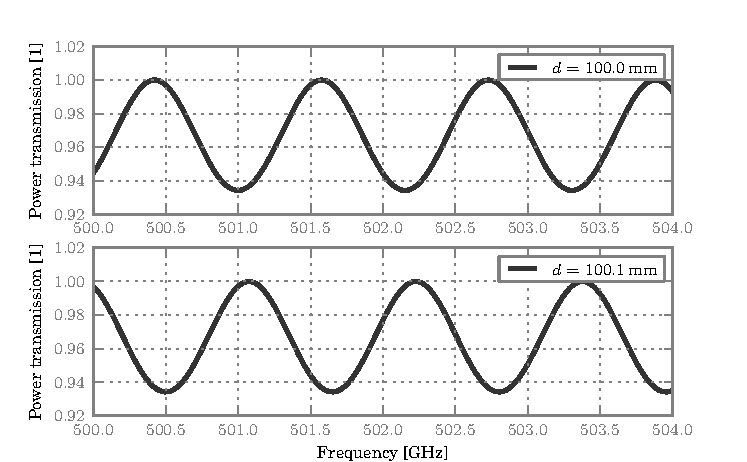
\includegraphics{cavity_sizes}
    \caption{Power transmission efficiency of two cavities of different lengths.}
    \caption*{
        When far from the frequency 0, a small change in the length $d$ of a cavity (here~\SI{0.1}{\percent}) has a strong influence on the ripple.
        The two ripples seem to have the same period but be out of phase.
        In fact, both have a phase of 0 and a slightly different period.
    }
    \label{fig:cavity_sizes}
\end{figure}



\subsubsection{Energy conservation}
In the previous section, we have concluded that some ratios between the wavelength and the length of the cavity produce destructive interferences: the detector does not receive any energy.
When this happens, where does the energy go?

The cavity does not store energy indefinitely in its standing wave.
Once the steady state is reached, the amplitude of the standing wave reaches a maximum.
After that, all the power that enters the cavity must either be dissipated, or exit the cavity.

\begin{figure}[hbtp]
    \centering
    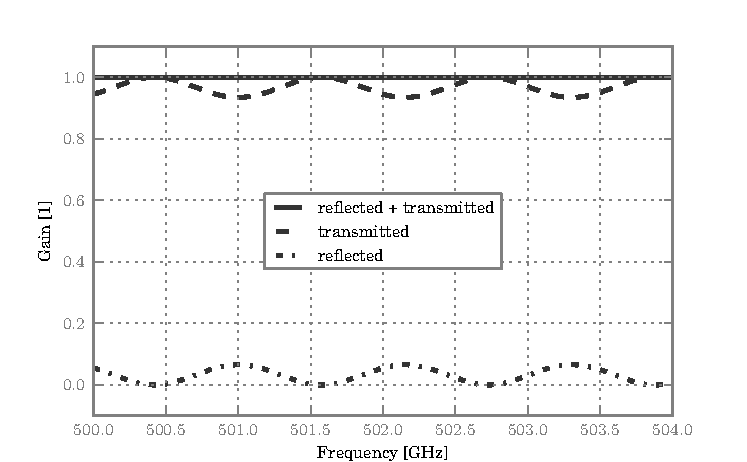
\includegraphics{cavity_energy_conservation}
    \caption{Power conservation in a lossless cavity.}
    \caption*{
        The power that enters a cavity can either be transmitted through the cavity, reflected by it, or anything in-between.
    }
    \label{fig:cavity_energy_conservation}
\end{figure}
We have spent the last few pages determining what the detector receives from the source.
It is linked to the transmission efficiency of the cavity that we have defined with~\cref{eq:cavity_transmission_efficiency}.
We have not paid much attention to the reflection efficiency of the cavity.
As one can guess, when the interferences are destructive on the detector-side of the cavity, they are constructive on the source-side: the energy is sent back to the source.
This is illustrated by~\cref{fig:cavity_energy_conservation}.
In order to create~\cref{fig:cavity_energy_conservation}, we had to use physically-plausible values for the reflection and transmission coefficients of the cavity.
This particular figure was produced using the refractive index \num{1} outside the cavity, \num{1.3} inside the cavity, and a cavity length of \SI{10}{\centi\meter}.
The reflection and transmissions coefficients were derived from the refractive indices using Fresnel's law for normal incidence~\eqref{eq:fresnel_normal}.

In a sense, a lossless cavity is an optical device that can be either totally transmissive, totally reflective, or anything in-between, depending on the frequency of the signal.


\subsubsection{Phase-amplitude degeneracy after folding by the mixer}
The output of a double-sideband mixer is the superposition of its lower-sideband and upper-sideband inputs multiplied by the mixer gain (see~\vref{fig:heterodyne_principle}).
A ripple, like any periodic signal, can be described as a sum of sinusoids.
Each sinusoid has an amplitude $a$, a period $F$ and a phase $\phi$.
\begin{align}
    \text{LSB} &= a \cos(2\pi(f_\text{LO} - f)/F + \phi)
    \\
    \text{USB} &= a \cos(2\pi(f_\text{LO} + f)/F + \phi)
\end{align}
These equations represent the output of the mixer at a frequency $f$ if only the LSB, or only the USB, receives power.
In this case we assume that the mixer gain is the same in both bands.
$f$ is the intermediate frequency and $f_\text{LO}$ the local oscillator frequency.
Therefore $f_\text{LO} - f$ is the lower sideband frequency (LSB) and $f_\text{LO} + f$ is the upper sideband frequency (USB).

The mixer folds the LSB on top of the USB.
The following equations show the effect that it has on the ripple.
\begin{gather}
    \text{DSB} = 
        a 
        \left[
            \cos \left( 2\pi(f_\text{LO} + f)/F + \phi \right)
            +
            \cos \left( 2\pi(f_\text{LO} - f)/F + \phi \right)
        \right]
    \\
    \begin{split}
    =
        2a
        \left[
            \cos \frac{2\pi(f_\text{LO} + f)/F + \phi + 2\pi(f_\text{LO} - f)/F + \phi}{2}
        \right.\\
        \left.
            \cos \frac{2\pi(f_\text{LO} + f)/F + \phi - 2\pi(f_\text{LO} - f)/F - \phi}{2}
        \right]
    \end{split}
    \\
    = 2a \cos(2\pi f_\text{LO}/F + \phi) \cos(2\pi f/F) \label{eq:folded_cos}
\end{gather}
\Cref{eq:folded_cos} shows that there is a degeneracy between the amplitude and the phase of a folded ripple.
A DSB ripple may have a small amplitude because the unfolded ripple has a low amplitude $a$, or because of the destructive interference $\cos(2\pi f_\text{LO} /F + \phi)$.

That degeneracy is important because it can help us.
If we try to fit a cosine to a ripple on a spectrum in order to determine its period, then this cosine has two parameters only: period and amplitude; the phase is known in advance to be 0.
This leads to a much more robust fitting of the period.
Indeed, if we refer to~\cref{fig:cavity_sizes}, we can understand how letting the phase free would very easily make the fit converge to an incorrect period.

In practice, it is likely that the mixer gain differs in LSB and USB, leading to a residual phase.
It is also possible that the ripple is not really periodic, but pseudo-periodic (its `period' is a function of frequency).
In these cases, there may be no degeneracy.

%#############################################################################

\section{Solver}
\label{sec:chapter2_3}

In this section, we present our method to solve for the output of a coherent optical system, while taking into account the infinity of reflections between every possible pair of optical components along every possible optical path.

A system like the Focal Plane Unit of HIFI comprises a few dozens of optical elements~\cite{jackson2002hifi}, referred in the literature as ``networks''~\cite{siegman1986lasers}: wire grid polarizers, roof-top mirrors, horns, attenuators, free space, all having one or more input and output.
All these networks interact together two by two since there exists at least one optical path between each pair or networks.

Two networks form one cavity.  Three networks form an infinite amount of cavities.

One way to solve a system's reaction to a set of input would be to propagate the inputs from network to network, back and forth, until the fields appear to converge to a steady state.
This would be an iterative solver.
Our solver is not iterative.
Instead, we propose a method to that directly provides the steady state.

%=============================================================================

\subsection{Scattering matrices}
Scattering matrices \cite{siegman1986lasers} model the transfer of power or field from one side (port) of a network to another (\cref{fig:scattering_matrix_notations}).
In coherent systems, they operate on phasors and therefore manipulate the field, not the power.

\Cref{eq:scattering_matrix} presents the scattering matrix $S$ that models the relation between a vector of inputs $a$ and a vector of outputs $b$ for a $n$-port network.
The diagonal contains the reflections terms and the rest contains the transmissions.
\begin{align}
    b &= S a
    &
    \begin{pmatrix}
        b_1\\
        b_2\\
        \vdots\\
        b_n
    \end{pmatrix}
    &=
    \begin{pmatrix}
        S_{1, 1} & S_{1, 2} & \cdots & S_{1, n} \\
        S_{2, 1} & S_{2, 2} & \cdots & S_{2, n} \\
        \vdots   & \vdots   & \ddots & \vdots   \\
        S_{n, 1} & S_{n, 2} & \cdots & S_{n, n}
    \end{pmatrix}
    \begin{pmatrix}
        a_1\\
        a_2\\
        \vdots\\
        a_n
    \end{pmatrix}
    \label{eq:scattering_matrix}
\end{align}

\begin{figure}[hbtp]
    \centering
    \input{scattering_matrix_notations.pdf_tex}
    \caption{A 4-port network showing four inputs $a_i$ and four outputs $b_i$.  For example, this network could be a wire grid polarizer or a semi-transparent mirror, both acting as beam splitters.}%
    \label{fig:scattering_matrix_notations}
\end{figure}

In the general case, scattering matrices cannot be multiplied together.
The scattering matrix of a system of two networks is not the product of the scattering matrices of the individual networks.
We will explore this further in \cref{sec:solving_a_system}.

Scattering matrices are firstly designed to model discrete physical optical elements such as interfaces, distances, horns, grids, etc.
It is possible to extend their use to an entire system made of several networks as long as it provides outputs that are linear combinations of inputs.
We will also explore this further in \cref{sec:solving_a_system}.



%=============================================================================
\subsection{Jones calculus in 3D}

%-----------------------------------------------------------------------------
\subsubsection{Traditional Jones calculus}
Jones matrices model the transfer of amplitude and phase from one polarization to another (see \citetitle{hecht2002optics} by ~\citeauthor{hecht2002optics}~\cite{hecht2002optics}).
In \cref{eq:jones_matrix_short}, the polarized input field $\vect{\hat{E}}_i$ is related to the polarized output field~$\vect{\hat{E}}_o$ by the Jones matrix $\hat{J}$.
$\vect{\hat{E}}_i$ and $\vect{\hat{E}}_o$ are called ``Jones vectors''.
\begin{equation}
    % Small form.
    \vect{\hat{E}}_o = \hat{J} \vect{\hat{E}}_i
    \label{eq:jones_matrix_short}
\end{equation}
The components of the Jones vectors are phasors: complex numbers that encode the amplitude and phase of the field along different axes (see~\cref{sec:phasors}).
The components of the Jones matrices are scalars, which encode changes in amplitude and phase.

\Cref{eq:jones_matrix_2d} presents the traditional form of Jones vectors and matrices, they are described in~\citetitle{hecht2002optics}.
\begin{equation}
    % Jones matrix in 2D.
    \begin{pmatrix}
        \hat{E}_{o, h}\\
        \hat{E}_{o, v}
    \end{pmatrix}
    =
    \begin{pmatrix}
        \hat{J}_{h, h}   &   \hat{J}_{h, v} \\
        \hat{J}_{v, h}   &   \hat{J}_{v, v}
    \end{pmatrix}
    \begin{pmatrix}
        \hat{E}_{i, h}\\
        \hat{E}_{i, v}
    \end{pmatrix}
    \label{eq:jones_matrix_2d}
\end{equation}
The field is seen as the superposition of a horizontal and a vertical component, both linearly polarized, noted $h$ and $v$.
The phase difference between these components determines the handedness and the ellipticity of the polarization of the field.

%-----------------------------------------------------------------------------
\subsubsection{Extension to three dimensions}
Although very useful for many applications, the traditional Jones matrices and vectors have limitations.
First, the field is always expressed in a local reference frame: the horizontal and vertical directions are valid for one beam only and may change after any reflection or refraction.
Therefore, to completely describe a field, the Jones vector is not enough since one needs to keep track of the orientation of its reference frame with three Euler angles, a quaternion or a rotation matrix.

Second, the horizontal and vertical directions are normal to each other and to the direction of propagation.
This limits us to modeling either transverse electric or transverse magnetic waves depending on whether the Jones vector represents the electric or the magnetizing field;
this cannot model hybrid waves, in which both the electric and the magnetizing field can have a component along the direction of propagation.
Therefore, this cannot model propagation in a birefringent material.
One way to accommodate this is to relax the constraint of orthogonality of the reference frame, allowing for the horizontal and vertical directions to have a component along the direction of propagation.
If we do this, then the full description of the field gets even more complicated as we need to carry along, not just the orientation of its reference frame, but the full description of that non-Cartesian reference frame.

Instead, we can express all the fields in a common global Cartesian reference frame, essentially extending Jones calculus from two to three dimensions, as illustrated in \cref{eq:jones_matrix_3d}.
\begin{equation}
    % Jones matrix in 3D.
    \begin{pmatrix}
        \hat{E}_{o, x}\\
        \hat{E}_{o, y}\\
        \hat{E}_{o, z}
    \end{pmatrix}
    =
    \begin{pmatrix}
        J_{x, x}   &   J_{x, y}   &   J_{x, z} \\
        J_{y, x}   &   J_{y, y}   &   J_{y, z} \\
        J_{z, x}   &   J_{z, y}   &   J_{z, z}
    \end{pmatrix}
    \begin{pmatrix}
        \hat{E}_{i, x}\\
        \hat{E}_{i, y}\\
        \hat{E}_{i, z}
    \end{pmatrix}
    \label{eq:jones_matrix_3d}
\end{equation}
These Jones matrices can be combined with rotation matrices (built from Euler angles or quaternions) in order to represent networks in any orientation in space.

%-----------------------------------------------------------------------------
\subsubsection{Rotating Jones matrices}
\label{sec:rotating_jones_matrices}
If $R$ is a 3--by--3 rotation matrix and $J$ the Jones matrix of a network at rest,
then \cref{eq:jones_rotation_using_inverse} gives the Jones matrix $J'$ corresponding to that network rotated by $R$.
\begin{equation}
    J' = R J R^{-1}
    \label{eq:jones_rotation_using_inverse}
\end{equation}
The multiplication by~$R^{-1}$ bring the electric field in the reference frame of the network at rest, so that we can apply~$J$.
The result is then rotated by $R$, which brings it back to the global reference frame.

\Cref{eq:jones_rotation_using_inverse} is mathematically correct, however it may not be the most practical to implement.
Indeed, inverting matrices is an expensive and unstable operation for a computer to perform
When we remember that the inverse of a rotation matrix is also its transpose,
then we get \cref{eq:jones_rotation_using_transpose} which has the advantage of being computationally cheap and stable.
\begin{equation}
    J' = R J R\transp
    \label{eq:jones_rotation_using_transpose}
\end{equation}

Rotating the identity matrix has an interesting property shown by~\eqref{eq:jones_rotation_identity}.
\begin{equation}
    I' = R I R^{-1}
       = R R^{-1}
       = I
    \label{eq:jones_rotation_identity}
\end{equation}
If a Jones matrix is proportional to an identity matrix, then it is not modified by rotation.
We will use that property to save some computation, for example when propagating through homogeneous isotropic materials (\vref{sec:generic_networks_distance}).



%=============================================================================
\subsection{Jones vectors and power}
\label{sec:jones_vectors_and_power}
When dealing with complex numbers, we must carefully define what we mean by ``power''.
\citetitle{IEEE2002dictionary} \cite{IEEE2002dictionary} defines the terms and SI units listed in~\cref{tab:complex_powers}.
\begin{table}[hbtp]
    \centering
    \begin{tabular}{lll}
        \toprule
        name & symbol & unit\\
        \midrule
        complex power     & $\hat{S} = P + iQ$\quad & \si{\volt\ampere} (volt-ampere) \\
        active/real power & $P \in \mathbb{R} = \Re(\hat{S})$\quad & \si{\watt} (watt) \\
        reactive power    & $Q \in \mathbb{R} = \Im(\hat{S})$\quad & \si{var} (volt-ampere-reactive) \\
        apparent power    & $\abs{\hat{S}} = \sqrt{P^2 + Q^2}$\quad & \si{\volt\ampere} (volt-ampere) \\
        \bottomrule
    \end{tabular}
    \caption{The four types of powers with complex signals.}
    \label{tab:complex_powers}
\end{table}

In our case, we deal with power densities: instead of watt, we use watt per square meter.
We can define ``complex power density'', ``active power density'', ``reactive power density'' and ``apparent power density'' by taking the correspondent powers from the list above and normalizing them by a unit surface area.
For simplicity, we keep the same notations.

Considering that the electric field is given in volt per meter and the magnetizing field in ampere per meter, their product yields a quantity that has the dimension of a power density.
\index{Poynting vector}The ``Poynting vector'' represents the directional energy flux density of an electromagnetic wave, typically expressed in \si{\watt\per\meter\squared} or \si{\volt\ampere\per\meter\squared}.
Traditionally noted~$\vect{\hat{S}}$, it is defined by \cref{eq:poynting_vector}.
\begin{equation}
    \vect{\hat{S}} \equaldef \frac{1}{2}\, \vect{\hat{E}} \times \vect{\hat{H}}^* \label{eq:poynting_vector}
\end{equation}
In~\cref{eq:poynting_vector}, the star symbol indicates an element-by-element complex conjugate, which we apply to a vector according to~\cref{eq:conjVect}.
\begin{equation}
    \vect{\hat{H}}^* = (\hat{H}_x^*, \hat{H}_y^*, \hat{H}_z^*)
    \label{eq:conjVect}
\end{equation}

The letter $S$ refers to the Poynting vector or the complex power, it has nothing to do with the $S$ referring to scattering matrices that we introduced earlier.
The alphabet has only so many letters.

The definition of this Poynting vector holds even for anisotropic propagation media for which $\vect{\hat{E}}$, $\vect{\hat{H}}$ and the wave vector $\vect{\hat{k}}$ may not be normal to each other.
Since the Poynting vector is defined by a cross product, it is by definition normal to the electric and magnetizing field, even if that direction differs from that of $\vect{\hat{k}}$.

This definition also holds for inhomogeneous waves.
Inhomogeneous waves are waves for which the real and the imaginary part of the wave vector point in different direction: they propagate in one direction but decay in another.
This behavior happens often in metal, and even in dielectrics in case of total internal reflection (more about this later when we mention Fresnel's equations).

If $\vect{\hat{e}}$ and $\vect{\hat{h}}$ are the electric and magnetizing phasors at a given location,
then the electric and magnetizing fields $\vect{\hat{E}}$ and $\vect{\hat{H}}$ at that location are functions of time~$t$ defined by~\cref{eq:e_h_time}.
The angular frequency $\omega$ is a real number because our systems are time-invariant.
\begin{subequations}
    \begin{align}
        \vect{\hat{E}} &= \vect{\hat{e}} \exp(-i \omega t) \\
        \vect{\hat{H}} &= \vect{\hat{h}} \exp(-i \omega t)
    \end{align}
    \label{eq:e_h_time}
\end{subequations}

Let us identify $\vect{\hat{S}} = \vect{\hat{E}} \times \vect{\hat{H}}^*$ with $\vect{\hat{S}} = \vect{P} + i\,\vect{Q}$.
\begin{subequations}
    \begin{align}
        \vect{\hat{S}}
        &= \frac{1}{2}\,\vect{\hat{E}} \times \vect{\hat{H}}^* \\
        &= \frac{1}{2}\,(\vect{E}_r + i\,\vect{E}_i) \times (\vect{H}_r - i\,\vect{H}_i) \\
        &= \underbrace{\frac{1}{2}\,(\vect{E}_r \times \vect{H}_r + \vect{E}_i \times \vect{H}_i)}_\vect{P} +\,
         i \underbrace{\frac{1}{2}\,(\vect{E}_i \times \vect{H}_r - \vect{E}_r \times \vect{H}_i)}_\vect{Q}
         \label{eq:SPQ_c}
    \end{align}
    \label{eq:SPQ}
\end{subequations}

We can use~\cref{eq:e_h_time} to compute the real and imaginary parts of $\vect{\hat{E}}$ and $\vect{\hat{H}}$ that appear in~\cref{eq:SPQ_c}.
To shorten the equations, we define $\hat{\tau}$, $\tau_r$ and $\tau_i$ quantities with~\cref{eq:tau_exptime}.
\begin{equation}
    \left\lbrace
        \begin{aligned}        
            \hat{\tau} &\equaldef \exp(-i \omega t) = \tau_r + i \tau_i\\
            \tau_r     &\equaldef \cos(-\omega t)\\
            \tau_i     &\equaldef \sin(-\omega t)
        \end{aligned}
    \right.
    \label{eq:tau_exptime}
\end{equation}
\begin{subequations}
    \begin{align}
        \vect{\hat{E}}
        &= \vect{\hat{e}} \hat{\tau}
        = (\vect{e}_r + i \vect{e}_i) (\tau_r + i \tau_i)
        =   \underbrace{(\vect{e}_r \tau_r - \vect{e}_i \tau_i)}_{\vect{E}_r}
        +\,i\underbrace{(\vect{e}_r \tau_i - \vect{e}_i \tau_r)}_{\vect{E}_i}
        \\
        \vect{\hat{H}}
        &= \vect{\hat{h}} \hat{\tau}
        = (\vect{h}_r + i \vect{h}_i) (\tau_r + i \tau_i)
        =   \underbrace{(\vect{h}_r \tau_r - \vect{h}_i \tau_i)}_{\vect{H}_r}
        +\,i\underbrace{(\vect{h}_r \tau_i - \vect{h}_i \tau_r)}_{\vect{H}_i}
    \end{align}
    \label{eq:ErEiHrHi}
\end{subequations}
\Cref{eq:ErEiHrHi} defines $\vect{E}_r$, $\vect{E}_i$, $\vect{H}_r$ and $\vect{H}_i$ that we can use in~\cref{eq:SPQ} to compute the active power density vector~$\vect{P}$ and the reactive one~$\vect{Q}$.
\begin{subequations}
    \begin{align}    
        \vect{P}
        &=
        \frac{1}{2}
        [
        (\vect{e}_r \tau_r - \vect{e}_i \tau_i) \times
        (\vect{h}_r \tau_r - \vect{h}_i \tau_i)
        +
        (\vect{e}_r \tau_i - \vect{e}_i \tau_r) \times
        (\vect{h}_r \tau_i - \vect{h}_i \tau_r)
        ]
        \\
        \vect{Q}
        &=
        \frac{1}{2}
        [
        (\vect{e}_r \tau_i - \vect{e}_i \tau_r) \times
        (\vect{h}_r \tau_r - \vect{h}_i \tau_i)
        -
        (\vect{e}_r \tau_r - \vect{e}_i \tau_i) \times
        (\vect{h}_r \tau_i - \vect{h}_i \tau_r)
        ]
    \end{align}
    \label{eq:PQ}
\end{subequations}
Before rushing to develop these equations, let us consider what we actually want to know.
The pointing vector is a function of time, it corresponds to an instantaneous power.
What we need is the time-averaged power.
We define the time-averaged Poynting vector $\langle\vect{\hat{S}}\rangle$ with~\cref{eq:avgS}.
\begin{equation}
    \langle\vect{\hat{S}}\rangle
    \equaldef
    \frac{1}{T}
    \int_0^T \! \vect{\hat{S}}(t)\, \mathrm{d}t
    \label{eq:avgS}
\end{equation}
In~\cref{eq:avgS}, $T$ is the period of the wave; $T = 1/f = 2\pi/\omega$.
The real and imaginary parts of $\vect{\hat{S}}$ are averaged independantly since 1 and $i$ form an orthogonal base, this gives us~\cref{eq:avgSPQ}.
\begin{equation}
    \langle\vect{\hat{S}}\rangle = \langle\vect{P}\rangle + i \langle\vect{Q}\rangle
    \label{eq:avgSPQ}
\end{equation}
In the expressions for the active and reactive power densities $\vect{P}$ and $\vect{Q}$ given in~\cref{eq:PQ}, the variables $\tau_r$ and $\tau_i$ are functions of the time $t$.
If we develop the cross-products of~\eqref{eq:PQ}, we reveal some terms in~$\tau_r^2=\cos^2$, some terms in $\tau_i^2=\sin^2$ and some terms in~$\tau_r \tau_i = \cos \cdot \sin$.
\Crefrange{eq:avgCos2}{eq:avgCosSin} give the time-average of these factors.
\begin{subequations}
    \begin{align}
        \langle \tau_r^2 \rangle
        &= \frac{1}{T} \int_0^T \! \cos(-2\pi t/T)^2\, \mathrm{d}t = \frac{1}{2}
        \label{eq:avgCos2}
    \\
        \langle \tau_i^2 \rangle
        &= \frac{1}{T} \int_0^T \! \sin(-2\pi t/T)^2\, \mathrm{d}t = \frac{1}{2}
        \label{eq:avgSin2}
    \\
        \langle \tau_r \tau_i \rangle
        &= \frac{1}{T} \int_0^T \! \cos(-2\pi t/T)\sin(-2\pi t/T)\, \mathrm{d}t = 0
        \label{eq:avgCosSin}
    \end{align}
\end{subequations}
\Cref{eq:avgCosSin} tells us that when we take the time-average of~\cref{eq:PQ}, we do not need to develop the terms in $\tau_r \tau_i$.
After developing and simplifying, we find that the time-averaged active and reactive powers density vectors are described by~\cref{eq:avgPQ}.
\begin{subequations}
    \begin{align}
        \langle\vect{P}\rangle
        &= \frac{1}{2}[\vect{e}_r \times \vect{h}_r + \vect{e}_i \times \vect{h}_i]
        \label{eq:avgP}
        \\
        \langle\vect{Q}\rangle
        &= \frac{1}{2}[\vect{e}_i \times \vect{h}_r - \vect{e}_r \times \vect{h}_i]
    \end{align}
    \label{eq:avgPQ}
\end{subequations}
As a final step, one can notice that $\langle\vect{P}\rangle$ and $\langle\vect{Q}\rangle$,
as defined in~\cref{eq:avgPQ}, are equal to one half the real and imaginary parts of the cross-product of phasors~$\vect{\hat{e}} \times \vect{\hat{h}}^*$.
Our final expression for the time-averaged power density vectors of a wave in a time-invariant and linear medium are given by~\cref{eq:avgSPQ_phasors} as functions of the electric and magnetizing phasors.
\begin{subequations}
    \begin{align}        
    \langle\vect{\hat{S}}\rangle &= \frac{1}{2}\,\vect{\hat{e}} \times \vect{\hat{h}}^*
    \\
    \langle\vect{P}\rangle       &= \frac{1}{2}\,\Re(\vect{\hat{e}} \times \vect{\hat{h}}^*)
    \\
    \langle\vect{Q}\rangle       &= \frac{1}{2}\,\Im(\vect{\hat{e}} \times \vect{\hat{h}}^*)
    \end{align}
    \label{eq:avgSPQ_phasors}
\end{subequations}

Let us call $\vect{s}$ the unit vector that points in the direction of the Poynting vector: $\vect{\hat{S}} = \hat{S} \vect{s}$.
This assumes that there is only one such unit vector: the real and imaginary part of the Poynting vector are collinear.
We also have $\vect{P} = P \vect{s}$
and $\vect{Q} = Q \vect{s}$.
The time-averaged active power from \cref{eq:avgP} can be projected onto that unit vector $\vect{s}$ to become \cref{eq:avgPproj}.
\begin{equation}
    \langle P \rangle
    = \frac{1}{2}
    [
        \norm{\vect{e}_r} \norm{\vect{h}_r}
        +
        \norm{\vect{e}_i} \norm{\vect{h}_i}
    ]
    \label{eq:avgPproj}
\end{equation}
In this equation, $\norm{\vect{\hat{v}}}$ represents the norm of the complex vector $\vect{\hat{v}}$, which we define as the square root of the dot product of the vector by itself, as shown in~\cref{eq:norm_complex_vector}.
\begin{equation}
    \norm{\vect{\hat{v}}}
    =
    \sqrt{\vect{\hat{v}} \cdot \vect{\hat{v}}}
    \label{eq:norm_complex_vector}
\end{equation}
That dot product itself is defined by~\cref{eq:inner_product} in which the star symbol represents the complex conjugation.
\begin{equation}   
    \vect{\hat{u}} \cdot \vect{\hat{v}} = \hat{u}_x \hat{v}_x^* + \hat{u}_y \hat{v}_y^* + \hat{u}_z \hat{v}_z^*
    \label{eq:inner_product}
\end{equation}

If we remember that the magnetizing and electric phasors are related by the admittance $\hat{Y}$ such that $\hat{h} = \hat{Y} \hat{e}$, and if we assume that this admittance has no imaginary component (propagation in a lossless material), then $\hat{h} = Y \hat{e}$.
This simplifies the previous equation by eliminating the magnetizing phasor.
\Cref{eq:avgPproj_lossless} gives the time-averaged active power density in the direction of propagation in a linear homogeneous and isotropic lossless material.
\begin{subequations}
    \begin{align}
        \langle P \rangle
        &=
        \frac{1}{2}
        [
            Y \norm{\vect{e}_r} \norm{\vect{e}_r}
            +
            Y \norm{\vect{e}_i} \norm{\vect{e}_i}
        ]
        \\
        &=
        \frac{1}{2} Y
        (\norm{\vect{e}_r}^2 + \norm{\vect{e}_i}^2)
        \\
        &=
        \frac{1}{2} Y
        \norm{\vect{\hat{e}}}^2
    \end{align}
    \label{eq:avgPproj_lossless}
\end{subequations}
This links the power of a wave to the square of its amplitude.

More generally, when the admittance has a complex value $\hat{Y} = Y_r + i Y_i$ then the time-averaged active power density is given by \cref{eq:avgPproj_lossful}.
\begin{equation}    
    \langle P \rangle
    =
    \frac{1}{2}
    \left(
        Y_r \norm{\vect{\hat{e}}}^2
        -
        Y_i \norm{\vect{e}_r} \norm{\vect{e}_i}
    \right)
\label{eq:avgPproj_lossful}
\end{equation}

In our last step, we define the notion of time-averaged power density efficiency.
It is the ratio of a time-averaged power density at two points in a system.
We can define it for the complex, active, reactive or apparent power, but the active one, $\langle P \rangle$, may be the more relevant to our interest.
Indeed, the sources that we observe emit real power and our detector detects real power.
When the two propagation media at the points $a$ and $b$ are lossless with the real admittances $Y_a$ and $Y_b$, then the time-averaged active power density efficiency is given by~\cref{eq:avgPeff_lossless}.
When they are not lossless, we need to use the more complete equation~\eqref{eq:avgPproj_lossful} on the numerator and denominator of our ratio.
\begin{equation}
    \frac{\langle P \rangle_b}{\langle P \rangle_a}
    =
    \frac{Y_b}{Y_a}
    \frac{\norm{\vect{\hat{e}}_b}^2}{\norm{\vect{\hat{e}}_a}^2}
    \label{eq:avgPeff_lossless}
\end{equation}

We define the field efficiency vector $\hat{\boldsymbol\eta}$ with~\cref{eq:field_efficiency_def}, using an element-wise multiplication of two vectors.
We do not use a symbol for that element-wise multiplication, we simply juxtapose the vectors.
\begin{equation}
    \vect{\hat{e}}_b
    = \boldsymbol{\hat{\eta}} \vect{\hat{e}}_a
    =
    \begin{pmatrix}
        \hat{\eta}_x \\ \hat{\eta}_y \\ \hat{\eta}_z
    \end{pmatrix}
    \begin{pmatrix}
        \hat{e}_{ax} \\ \hat{e}_{ay} \\ \hat{e}_{az}
    \end{pmatrix}
    =
    \begin{pmatrix}
        \hat{\eta}_x \hat{e}_{ax} \\
        \hat{\eta}_y \hat{e}_{ay} \\
        \hat{\eta}_z \hat{e}_{az}
    \end{pmatrix}
    \label{eq:field_efficiency_def}
\end{equation}
The complex conjugation is distributive with respect to the multiplication ($(uv)^* = u^* v^*$), which allows us to write the following equality.
\begin{equation}
    \vect{\hat{e}}^*_b
    = \boldsymbol{\hat{\eta}}^* \vect{\hat{e}}^*_a
    =
    \begin{pmatrix}
        \hat{\eta}^*_x \\ \hat{\eta}^*_y \\ \hat{\eta}^*_z
    \end{pmatrix}
    \begin{pmatrix}
        \hat{e}^*_{ax} \\ \hat{e}^*_{ay} \\ \hat{e}^*_{az}
    \end{pmatrix}
    =
    \begin{pmatrix}
        \hat{\eta}^*_x \hat{e}^*_{ax} \\
        \hat{\eta}^*_y \hat{e}^*_{ay} \\
        \hat{\eta}^*_z \hat{e}^*_{az}
    \end{pmatrix}
    \label{eq:field_efficiency_conj}
\end{equation}
However, this field efficiency is not easily converted into a power efficiency.
\begin{subequations}
    \begin{align*}
        \norm{\vect{\hat{e}}_b}^2
        &=
        \vect{\hat{e}}_b \cdot \vect{\hat{e}}_b
        \\
        &=
        \hat{\eta}_x \hat{e}_{ax} \hat{\eta}^*_x \hat{e}^*_{ax} +
        \hat{\eta}_y \hat{e}_{ay} \hat{\eta}^*_y \hat{e}^*_{ay} +
        \hat{\eta}_z \hat{e}_{az} \hat{\eta}^*_z \hat{e}^*_{az}
        \\
%        &=
%        \hat{\eta}_x \hat{\eta}^*_x \hat{e}_{ax} \hat{e}^*_{ax} +
%        \hat{\eta}_y \hat{\eta}^*_y \hat{e}_{ay} \hat{e}^*_{ay} +
%        \hat{\eta}_z \hat{\eta}^*_z \hat{e}_{az} \hat{e}^*_{az}
%        \\
        &\neq
        \cancel{
            \norm{\boldsymbol{\hat{\eta}}}^2
            \norm{\vect{\hat{e}}_a}^2
        }
    \end{align*}
\end{subequations}
Squaring the field efficiency to get a power efficiency would be a mistake in the general case.


%=============================================================================
\subsection{Combining scattering and Jones matrices}
We repeat here the definition of a scattering matrix given by \vref{eq:scattering_matrix}.
In this equation, all the scalars are complex.
\begin{align*}
    b &= S a
    &
    \begin{pmatrix}
        b_1\\
        b_2\\
        \vdots\\
        b_n
    \end{pmatrix}
    &=
    \begin{pmatrix}
        S_{1, 1} & S_{1, 2} & \cdots & S_{1, n} \\
        S_{2, 1} & S_{2, 2} & \cdots & S_{2, n} \\
        \vdots   & \vdots   & \ddots & \vdots   \\
        S_{n, 1} & S_{n, 2} & \cdots & S_{n, n}
    \end{pmatrix}
    \begin{pmatrix}
        a_1\\
        a_2\\
        \vdots\\
        a_n
    \end{pmatrix}
\end{align*}

Since Jones vectors describe polarized waves, we had the idea of modeling each input and output with a Jones vector.
Each port of an optical network receives and emits a polarized wave.
This makes $a$ and $b$ vectors of Jones vectors.
As a consequence, each element $S_{i, j}$ of the scattering matrix S is a Jones matrix.
We are dealing with vectors of vectors and matrices of matrices, as shown by \cref{eq:matrix_of_matrices} for a 2-port network.

\begin{equation}
    \begin{gathered}
    \begin{pmatrix}
        \begin{pmatrix}
            b_{1, x} \\ b_{1, y} \\ b_{1, z}
        \end{pmatrix}
        \\
        \begin{pmatrix}
            b_{2, x} \\ b_{2, y} \\ b_{2, z}
        \end{pmatrix}
    \end{pmatrix}
    =
    S
    \begin{pmatrix}
        \begin{pmatrix}
            a_{1, x} \\ a_{1, y} \\ a_{1, z}
        \end{pmatrix}
        \\
        \begin{pmatrix}
            a_{2, x} \\ a_{2, y} \\ a_{2, z}
        \end{pmatrix}
    \end{pmatrix}
    \\
    S =
    \begin{pmatrix}
        \begin{pmatrix}
            S_{1, 1, x, x} & S_{1, 1, x, y} & S_{1, 1, x, z} \\
            S_{1, 1, y, x} & S_{1, 1, y, y} & S_{1, 1, y, z} \\
            S_{1, 1, z, x} & S_{1, 1, z, y} & S_{1, 1, z, z} \\
        \end{pmatrix}
        &
        \begin{pmatrix}
            S_{1, 2, x, x} & S_{1, 2, x, y} & S_{1, 2, x, z} \\
            S_{1, 2, y, x} & S_{1, 2, y, y} & S_{1, 2, y, z} \\
            S_{1, 2, z, x} & S_{1, 2, z, y} & S_{1, 2, z, z} \\
        \end{pmatrix}
        \\
        \begin{pmatrix}
            S_{2, 1, x, x} & S_{2, 1, x, y} & S_{2, 1, x, z} \\
            S_{2, 1, y, x} & S_{2, 1, y, y} & S_{2, 1, y, z} \\
            S_{2, 1, z, x} & S_{2, 1, z, y} & S_{2, 1, z, z} \\
        \end{pmatrix}
        &
        \begin{pmatrix}
            S_{2, 2, x, x} & S_{2, 2, x, y} & S_{2, 2, x, z} \\
            S_{2, 2, y, x} & S_{2, 2, y, y} & S_{2, 2, y, z} \\
            S_{2, 2, z, x} & S_{2, 2, z, y} & S_{2, 2, z, z} \\
        \end{pmatrix}
    \end{pmatrix}
    \end{gathered}
    \label{eq:matrix_of_matrices}
\end{equation}

Although matrices of matrices are compatible with simple algebraic operations (the product above follows the usual rule for multiplying matrices), we prefer to interpret them as more conventional ``block matrices''.
Block matrices are described by \citeauthor{eves2012elementary} in \citetitle{eves2012elementary} \cite{eves2012elementary}.
They are conventional matrices, in the sense that they hold scalars, but they are subdivided in regions, or ``blocks''.
Mathematically, \cref{eq:matrix_of_matrices} is equivalent to \cref{eq:matrix_flattenned}.
\begin{equation}
    \begin{pmatrix}
        b_{1, x} \\ b_{1, y} \\ b_{1, z}
        \\
        b_{2, x} \\ b_{2, y} \\ b_{2, z}
    \end{pmatrix}
    =
    \begin{pmatrix}
        S_{1, 1, x, x} & S_{1, 1, x, y} & S_{1, 1, x, z}   &   S_{1, 2, x, x} & S_{1, 2, x, y} & S_{1, 2, x, z} \\
        S_{1, 1, y, x} & S_{1, 1, y, y} & S_{1, 1, y, z}   &   S_{1, 2, y, x} & S_{1, 2, y, y} & S_{1, 2, y, z} \\
        S_{1, 1, z, x} & S_{1, 1, z, y} & S_{1, 1, z, z}   &   S_{1, 2, z, x} & S_{1, 2, z, y} & S_{1, 2, z, z} \\
        S_{2, 1, x, x} & S_{2, 1, x, y} & S_{2, 1, x, z}   &   S_{2, 2, x, x} & S_{2, 2, x, y} & S_{2, 2, x, z} \\
        S_{2, 1, y, x} & S_{2, 1, y, y} & S_{2, 1, y, z}   &   S_{2, 2, y, x} & S_{2, 2, y, y} & S_{2, 2, y, z} \\
        S_{2, 1, z, x} & S_{2, 1, z, y} & S_{2, 1, z, z}   &   S_{2, 2, z, x} & S_{2, 2, z, y} & S_{2, 2, z, z}
    \end{pmatrix}
    \begin{pmatrix}
        a_{1, x} \\ a_{1, y} \\ a_{1, z}
        \\
        a_{2, x} \\ a_{2, y} \\ a_{2, z}
    \end{pmatrix}
    \label{eq:matrix_flattenned}
\end{equation}

This equivalence means that we can see each polarization of each port as a full-fledged port, and that the same physical phenomenon could be modeled with a 6-port network described by \cref{eq:matrix_totally_flattenned}.
\begin{equation}
    \begin{pmatrix}
        b'_1 \\ b'_2 \\ b'_3 \\ b'_{4} \\ b'_{5} \\ b'_{6}
    \end{pmatrix}
    =
    \begin{pmatrix}
        S'_{1, 1} & S'_{1, 2} & S'_{1, 3} & S'_{1, 4} & S'_{1, 5} & S'_{1, 6} \\
        S'_{2, 1} & S'_{2, 2} & S'_{2, 3} & S'_{2, 4} & S'_{2, 5} & S'_{2, 6} \\
        S'_{3, 1} & S'_{3, 2} & S'_{3, 3} & S'_{3, 4} & S'_{3, 5} & S'_{3, 6} \\
        S'_{4, 1} & S'_{4, 2} & S'_{4, 3} & S'_{4, 4} & S'_{4, 5} & S'_{4, 6} \\
        S'_{5, 1} & S'_{5, 2} & S'_{5, 3} & S'_{5, 4} & S'_{5, 5} & S'_{5, 6} \\
        S'_{6, 1} & S'_{6, 2} & S'_{6, 3} & S'_{6, 4} & S'_{6, 5} & S'_{6, 6}
    \end{pmatrix}
    \begin{pmatrix}
        a'_1 \\ a'_2 \\ a'_3 \\ a'_{4} \\ a'_{5} \\ a'_{6}
    \end{pmatrix}
    \label{eq:matrix_totally_flattenned}
\end{equation}
Although the term is not canon, we decide to call non-block matrices ``flat'' matrices.
They are flat in the sense that they are two dimensional, while our block matrices have four indices and are therefore four-dimensional.
In this book, we will switch between block matrices and flat matrices at our convenience.

It is possible that tensor calculus could have helped us here.
Block matrices could be replaced by tensors of order 4.
Tensors unify scalars, vectors, matrices and higher-order `array'-like structures.
We have not investigated the the advantages of tensor calculus for our model.
Switching between block and flat matrices is easy enough.


%=============================================================================
\subsection{Solving a system}
\label{sec:solving_a_system}
Now that we have defined a mathematical object that holds all the necessary information to deal with amplitude, phase, polarization and orientation in space for a network with an arbitrary amount of ports (the scattering matrix of Jones matrices), we are ready to solve a system containing any number network.

%-----------------------------------------------------------------------------
\subsubsection{Theory}

Assume a coherent optical system.
We call $S$ the flat scattering matrix of the entire system.
\begin{equation*}
    S =
    \begin{pmatrix}
        S_{1, 1} & S_{1, 2} & \cdots & S_{1, n} \\
        S_{2, 1} & S_{2, 2} & \cdots & S_{2, n} \\
        \vdots   & \vdots   & \ddots & \vdots \\
        S_{n, 1} & S_{n, 2} & \cdots & S_{n, n}
    \end{pmatrix}
\end{equation*}
\begin{equation*}
    b = Sa
\end{equation*}
$S$ contains information about all the ports in the system: the ports that are open to the outside world, but also the ports hidden within the system because the networks are coupled to each other.
Here, $n$ is the number of ports of $S$, equal to the sum of the number of ports of all the networks constituting the system.

In the rest of this section, the components of vectors and matrices are are implicitly complex.
In order to lighten the notations, we will not place the hat symbol which we usually use for complex numbers.

\begin{figure}[hbtp]
    \centering
    \input{output_g_is_input_h.pdf_tex}
    \caption{Two networks coupled by one port: the output of one is the input of the other.}
    \caption*{
        The port~$g$ of network~G is coupled to the port~$h$ of network~H.
        Input phasors are labeled~$a$ and output phasors are labeled~$b$.
        The subscripts of $a$ and $b$ refer to the label of the port.
    }
    \label{fig:output_g_is_input_h}
\end{figure}

Some of the networks constituting the system are coupled by one port.
If two networks G and H are coupled by their port $g$ and $h$ (see~\cref{fig:output_g_is_input_h}), then the output phasor of $g$ is the input phasor of $h$ and the output phasor of $h$ is the input phasor of $g$, as illustrated by \cref{eq:coupled_inputs_outputs}.
\begin{equation}
    \left\lbrace
    \begin{aligned}
        b_h &= a_g \\
        b_g &= a_h
    \end{aligned}
    \right.
    \label{eq:coupled_inputs_outputs}
\end{equation}

Three rules: First, if a port~$i$ is coupled to a port~$j$, then~$j$ is coupled to~$i$.
Second, a port can be coupled to zero or one other port, not more.
Third, a port must not be coupled to itself.
The third rule might not be necessary from a mathematical point of view, but it makes little sense physically and it simplifies slightly the implementation of some algorithms of~\cref{sec:solver_implementation}.
For these rules, the network to which a port belong do not matter: we can couple two different ports of the same network, or we can couple two networks several times with different pairs of ports.

Ports that are coupled are called ``inside port'', those that are not coupled are called ``outside port''.
If we note~$a^o$ the inputs from the outside world,~$b^o$ the outputs to the outside world,~$a^i$ the inputs inside the system and~$b^i$ the outputs inside the system, then we can reorder the rows and columns of the vectors~$a$,~$b$ and the matrix~$S$ to put together the inside ports and the outside ports.
This is illustrated by \cref{eq:s_outside_inside} with block matrices separating the inside and outside ports.
\begin{align}
    b&=Sa
    &
    \binom{b^o}{b^i} &=
    \begin{pmatrix}
        S^{oo} & S^{oi} \\
        S^{io} & S^{ii} \\
    \end{pmatrix}
    \binom{a^o}{a^i}
    \label{eq:s_outside_inside}
\end{align}

The four blocks of~$S$ have the following physical meaning:

\begin{table}[H]
    \centering
    \begin{tabularx}{\textwidth}{l l X}
        $S^{oo}$ & from outside to outside & Signal that is reflected on the entrance ports and therefore never enters the system.\\
        $S^{io}$ & from outside to inside & Signal that enters the system.\\
        $S^{ii}$ & from inside to inside & Transmissions and reflections internal to the system.\\
        $S^{oi}$ & from inside to outside & Signal that leaves the system.\\
    \end{tabularx}
\end{table}

Of $a$ and $b$, only~$a^o$ is known: this corresponds to the input to the system and we control it.
$a^i$,~$b^i$ and~$b^o$ are unknown.
$b^o$ is the result for which we are looking.
$b^i$ and~$a^i$ are nice to have as they allow us to see what is happening inside the system.

\paragraph{Solving the internal transmissions and reflections.}
How are~$a^i$ and~$b^i$ related?
\Cref{eq:coupled_inputs_outputs} indicates that each element of $a^i$ is equal to an element of $b^i$, therefore $a^i$ can be obtain by reordering $b^i$ and vice-versa.
\index{permutation matrix}In other words, there exists a permutation matrix~$P$ such that
\begin{equation}
    a^i = P b^i \text{.} \label{eq:relation_ai_bi}
\end{equation}

Permutation matrices permute the order of rows and columns of matrices.
They contain one and only one 1 per row and per column, all the other elements are~0.
Pre-multiplying by a permutation matrix changes the order of the rows.
Post-multiplying by a permutation matrix changes the order of the columns.
The transpose of a permutation matrix is also a permutation matrix.
The transpose of a permutation matrix is also its inverse: $P\transp = P^{-1}$.
This last property is important when implementing the algorithm because inverting matrices is expensive and unstable.

To get $b^o$, the first step is to compute~$b^i$ from~$a^o$.
\begin{subequations}
    \begin{align}
        b^i &= S^{io}a^o + S^{ii}a^i \label{eq:compute_bi_ai} \\
        b^i &= S^{io}a^o + S^{ii}Pb^i \label{eq:compute_bi_bi} \\
        (I - S^{ii}P)b^i &= S^{io}a^o \label{eq:compute_bi_solve} \\
        b^i &= (I - S^{ii}P)^{-1} S^{io}a^o \label{eq:compute_bi_invert}
    \end{align} \label{eq:compute_bi}
\end{subequations}
where~$I$ is the identity matrix with a dimension equal to that of~$S^{ii}P$.

Can we go from \cref{eq:compute_bi_solve} to \cref{eq:compute_bi_invert}?
The matrix~$I - S^{ii}P$ has an inverse if and only if it is not singular.
A matrix is singular if and only if its determinant equals~0.
Can the determinant of~$I - S^{ii}P$ equal~0 (\cref{eq:det_i_minus_siip})?
\begin{equation}
    \det(I - S^{ii}P) = 0 \label{eq:det_i_minus_siip}
\end{equation}
\index{eigenvalue}\Cref{eq:det_i_minus_siip} has the shape of an eigenvalue problem;
\cref{eq:eigenvalue_typical} defines the eigenvalues~$\lambda$ of a matrix~$A$.
\begin{equation}
    \det(A - \lambda I) = 0 \label{eq:eigenvalue_typical}
\end{equation}
In our case, $\lambda=1$ and $A=S^{ii}P$.
However, the sign is not the same: $I-A \neq A-I$.
Fortunately, the determinant has the following property \cref{eq:determinant_scalar_multiplication}:
\begin{equation}
    \det(c A) = c^n \det(A) \label{eq:determinant_scalar_multiplication}
\end{equation}
for any $n$--by--$n$ matrix $A$.
Therefore,
\begin{subequations}
    \begin{align}
        \det(I - S^{ii}P)
        &= \det(-1(S^{ii}P - I)) \\
        &= (-1)^n \det(S^{ii}P - I) \text{.}
    \end{align}
\end{subequations}
We do not need to worry about the parity of~$n$.
Indeed, if $x=0$ then $(-1)^n x = 0$ as well.
This means that for our eigenvalue problem, the sign does not matter, as summarized by \cref{eq:determinant_sign_does_not_matter}.
\begin{equation}
    \det(I - S^{ii}P) = 0
    \quad
    \Longleftrightarrow
    \quad
    \det(S^{ii}P - I) = 0
    \label{eq:determinant_sign_does_not_matter}
\end{equation}
\index{eigenvector}We have successfully identified our question of the invertibility of $I - S^{ii}P$ with a question regarding the eigenvectors of $S^{ii}P$ for the eigenvalue 1.
Saying $\det(S^{ii}P - I) = 0$ is equivalent to saying that there exist non-zero vectors $v$, called ``eigenvectors'', such that $v = S^{ii}Pv$.
The following argument, based on physical considerations, will demonstrate that there are no such vectors.

$b^i$ is what $S^{ii}P$ is applied to in \cref{eq:compute_bi}, therefore we are looking for vectors $b^i$ satisfying
\begin{equation}
    b^i = S^{ii}P b^i \text{.} \label{eq:bi_eigenvector}
\end{equation}
The two equations \cref{eq:bi_eigenvector} and  \cref{eq:compute_bi_bi}, taken together, 
lead to the following interesting equality:
\begin{equation}
    \left\lbrace
        \begin{aligned}
            b^i &= S^{ii}P b^i \\
            b^i &= S^{io}a^o + S^{ii}P b^i
        \end{aligned}
    \right.
    \quad
    \Longleftrightarrow
    \quad
    S^{io}a^o = 0
\end{equation}
The only way for $S^{io}a^o$ to equal 0 for any value of $a^o$ is for $S^{io}$ to contain only zeros.
In other words, the system is totally blind: no energy from the outside world ($a^o$) ever enters the system.
Blind systems cannot be solved by our method but this is not a problem since there is no point in trying to build them in the first place.
For the rest of this demonstration, let us assume that the system is not blind, $S^{io}\neq 0$, but that instead we merely set $a^o$ to 0; let us also assume $b^i \neq 0$ (we somehow managed to inject energy inside the system before switching off the source $a^o$).
What would $b^i = S^{ii}P b^i$ mean?

$b^i$ is the list of all the outputs of the inside part of the system, fed back as input to that same system.
What \cref{eq:bi_eigenvector} means is that there exists some fields that are unaffected by the system; if such a field would enter the system, it would be trapped inside the system, looping through $S^{ii}P$ forever.
If $S^{ii}P$ has an eigenvector, then our system is totally lossless (for some fields) and can store any amount of energy forever.
We know that all our networks have losses; even the propagation in free space has losses in the form of the beam diffracting slowly and becoming wider than its target, essentially leaking energy.
Without using active components (external energy source, amplifiers), the best we can do is to aim for very low losses, which would produce very high-quality cavities but not perpetual storages.
Because our systems have losses, $S^{ii}P$ has no eigenvectors.
Therefore $S^{ii}P$ has no eigenvalues.
Therefore 1 is not an eigenvalue.
Therefore $\det(I-S^{ii}P) \neq 0$.
Therefore $I-S^{ii}P$ has an inverse.
Therefore \cref{eq:compute_bi_invert} is correct, and the system can be solved.

It can be interesting to draw a parallel between our problem and the convergence of an infinite geometric series.
Indeed, the sum of an infinite series of ratio $q$ converges if $\abs{q} < 1$ (whether $q$ is real or complex):
\begin{equation}
    \sum_{i=0}^\infty q^i = \frac{1}{1-q} = (1-q)^{-1}
\end{equation}
The resemblance with $(I - S^{ii}P)^{-1}$ is not due to chance.
Our system acts like a cavity, maybe a very complex cavity but a cavity nonetheless.
Therefore we can think about it as a simple cavity delimited by two semi-transparent mirrors.
The signal trapped inside the cavity is reflected an infinite amount of times, each double-reflection attenuates the signal by a factor $q=S^{ii}P$.
As a result, the signal inside the cavity is the signal that enters the cavity multiplied by $1+q+q^2+q^3+\dots$ up to infinity.
If there are losses, then $|q|<1$ and that series converges to $(1-q)^{-1}$ or, considering we are working with matrices, $(I - S^{ii}P)^{-1}$.

Note that for the implementation, we may want to avoid inverting the matrix.
Indeed, inverting matrices is costly and numerically unstable.
Even though \cref{eq:compute_bi_invert} is mathematically correct, we would rather solve $b^i$ in \cref{eq:compute_bi_solve}.

\paragraph{Solving the output of the system.}
Once we know the internal reflections of the system ($b^i$ as a function of itself), getting its output is trival.
The second step is to compute~$b^o$ from~$a^o$ and~$b^i$.
We do that by taking $b^o$ from \cref{eq:s_outside_inside} and eliminating $a^i$ with \cref{eq:relation_ai_bi}.
\begin{align}
    b^o &= S^{oo}a^o + S^{oi}a^i \\
    b^o &= S^{oo}a^o + S^{oi}Pb^i \label{eq:compute_bo}
\end{align}

These two steps solve the system: from the inputs~$a^o$ we can compute the outputs~$b^o$ of the whole system.
This method also gives us $a^i$ and $b^i$ which are two equivalent ways of looking at what is happening inside the system (they are permutations of each other).



\paragraph{Internal sources.}
The method described above does not allow us to account for sources inside the system.
Such sources may nevertheless exist.
For example, the local oscillator of HIFI is located outside the cryostat (\cref{fig:internal_sources_windows}).
Therefore, the local oscillator is warmer, radiating heat.
With the current state of our model, we can make this local oscillator power an external source.
However, the windows that physically separate the cryostat from the outside world are also relatively warm, and they also act as sources of radiation.

\begin{figure}[hbtp]
    \centering
    \input{cryostat_window.pdf_tex}
    \caption{The cryostat windows are warm enough to emit a significant power.}
    \caption*{
        Planck's law relates the physical temperature of matter to the electromagnetic radiation it emits.
        In HIFI, the local oscillator is outside the cryostat and therefore relatively warm.
        The cryostat has a transparent window that lets the LO beam through (the window is tilted to avoid standing waves).
        The window, being between a warm and a cold environment, is subject to a strong gradient of temperature; calculating its emission is a problem of radiative transfer.}
    \label{fig:internal_sources_windows} 
\end{figure}

Let us assume that every port radiates a constant field described by \cref{eq:internal_sources}.
The output $b_i$ of a port is a linear combination of the inputs $a_j$, plus a constant emission $c_i$.
\begin{equation}
    b = S a + c
    \label{eq:internal_sources}
\end{equation}
The separation into inside and outside ports is straight forward, as \cref{eq:internal_sources_io} indicates.
\begin{equation}
    \begin{pmatrix}
        b^o\\
        b^i\\
    \end{pmatrix}
    =
    \begin{pmatrix}
        S^{oo} & S^{oi} \\
        S^{io} & S^{ii}
    \end{pmatrix}
    \begin{pmatrix}
        a^o\\
        a^i\\
    \end{pmatrix}
    +
    \begin{pmatrix}
        c^o\\
        c^i\\
    \end{pmatrix}
    \label{eq:internal_sources_io}
\end{equation}
Like previously, we solve for the internal transmissions and reflections.
\begin{subequations}
    \begin{align}
        b^i &= S^{io} a^o + S^{ii} a^i + c^i \label{eq:compute_bi_ai_ci}\\
        b^i &= S^{io} a^o + S^{ii} Pb^i + c^i \label{eq:compute_bi_bi_ci}\\
        (I - S^{ii} P) b^i &= S^{io} a^o + c^i \label{eq:compute_bi_ci_solve}
    \end{align}
    \label{eq:compute_bi_ci}
\end{subequations}
\Cref{eq:compute_bi_ci_solve} is very similar to \cref{eq:compute_bi_solve} and is as easy to solve for~$b^i$.
The previous discussion regarding the invertibility of $(I - S^{ii} P)$, through the meaning of \cref{eq:bi_eigenvector}, still applies here.

Once $b_i$ is known, we inject its value into the expression of $b^o$.
\begin{subequations}
    \begin{align}
        b^o &= S^{oo} a^o + S^{oi} a^i + c^o \label{eq:compute_bo_ai_co}\\
        b^o &= S^{oo} a^o + S^{oi} Pb^i + c^o \label{eq:compute_bo_bi_co}
    \end{align}
    \label{eq:compute_bo_co}
\end{subequations}
Equations~\eqref{eq:compute_bi_ci_solve} and~\eqref{eq:compute_bo_bi_co} give us the response $b$ of the system $(S, P)$ to the inputs $a$ and $c$.


%-----------------------------------------------------------------------------
\paragraph{Solving for each source independently.}
\label{solving_for_each_source_independently}
When solving a system with multiple sources, it may be tempting to set all the inputs at the same time.
That is, filling $a^o$ and $c$, then computing $b$.
This is, in most cases, a mistake.
If two inputs are set at the same time, then they act as if they are phase-locked to each other, which introduces interferences that cannot be produced with either input source off.
Unless the sources are actually phase-locked to each other, the proper way of calculating the response of the system is to solve it for each source individually.

In the case of HIFI, the radiation for the local oscillator, the cryostat windows, the calibration loads and the sky must be solved separately, then added in power.

As explained earlier, sources that are a priori incoherent become coherent when the bandwidth is narrow enough.
In HIFI, the bandwidth is narrower than \SI{1}{\mega\hertz}
which gives a coherence time $t_c = 1/\SI{1}{\mega\hertz} \approx \SI{1}{\microsecond}$.
This means that, for a duration of~\SI{1}{\micro\second}, the signal coming from the astronomical object, or the thermal noise coming from the local oscillator or the calibration black bodies, will be coherent.
As such, it has a polarization and a phase.
We can decompose the polarization of that wave on any convenient base, for example an orthonormal $(\vect{u_x}, \vect{u_y})$ base.
This allows us to describe the wave with \cref{eq:incoherent_decomposed}.
\begin{equation}
    \vect{E} = E_0 \cos(kz - \omega t + \phi_x) \vect{u_x}
             + E_0 \cos(kz - \omega t + \phi_y) \vect{u_y}
    \label{eq:incoherent_decomposed}
\end{equation}
What makes the wave incoherent is that $\phi_x$ and $\phi_y$ are random.
They are random, but they change relatively slowly with time (at the scale of the microsecond in HIFI).

The $x$ and $y$ components are always coherent because they are correlated with themselves (trivial), even after one microsecond.
However, there is a priori no correlation between the $x$ and $y$ components.
This absence of correlation blurs all interferences between $x$ and $y$ after one microsecond.
A typical HIFI observation integrates on the sky for about one second, which is a million times more than the coherence time.
As a result, the $x$ and $y$ components of the incoming wave can, and must, be treated independently.
The two components of a incoherent wave must be treated as two independent coherent signal.

The base that we choose for decomposing the polarization does not matter, what matters is that we decompose it.
We can model an incoherent source of power $P$ by modeling two coherent sources of power $P/2$ of opposite polarizations.
We simulate both sources separately, then add the results in power (not in field).
The polarizations can be horizontal and vertical, or clockwise and anticlockwise.

If a source is partially polarized, then we refer the reader to~\citetitle{goodman1985statistical} by \citeauthor{goodman1985statistical} \cite{goodman1985statistical}, which explains describes and details all of this.



%-----------------------------------------------------------------------------
\subsubsection{Implementation}
\label{sec:solver_implementation}
Although the mathematics are quite simple, the implementation requires careful book keeping of the many indices of the many matrices.
In order to make this section less abstract and easier to follow, let us consider the very simple system made of three networks that is shown in~\cref{fig:implementation_0}.
This system represents the simplest heterodyne telescope that can be built.
The sky and the local oscillator emit a signal (red arrows).
A semi-transparent beam splitter combines the signal from the sky and the signal from the local oscillator.
The beam splitter is mostly transparent, barely reflective, so that most of the signal from the sky couples to the mixer.
As a side effect, most of the signal from the local oscillator is lost but a small fraction of it shines onto the mixer.
The detector detects a signal (green arrow).

Let us ignore, for the sake of simplicity, that the electric field is in three dimensions.
Using vectors would triple the number of ports, which would be more realistic, but the principle works perfectly well with one dimension only.
In our example, our networks exchange a single scalar.

\begin{figure}[hbtp]
    \centering
    \input{implementation_0.pdf_tex}
    \caption{A system made of three networks.}
    \label{fig:implementation_0}
\end{figure}

\begin{itemize}
    \item 
The system contains $N$ networks.
\\In our example, $N=3$.
    \item 
Each network is modeled with a~$n_i$--by--$n_i$ scattering matrix, where~$n_i$ is the number of ports the network $i$, with $i \in \llbracket 1, N \rrbracket$.
\\
The beam splitter of our example is a four-port networks: $n_1=4$.
The local oscillator has one port only: $n_2=1$.
The mixer has two: $n_3=2$.
We are not interested in the content of these matrices at this point, let us just assume that we can compute them from relevant parameters.
    \item 
The whole system is modeled with a~$n$--by--$n$ scattering matrix, where~$n$ is the number of ports of the whole system, with $n = \sum_{i=1}^N n_i$.
\\
In our example, $n=4+1+2=7$.
\end{itemize}

\begin{figure}[hbtp]
    \centering
    \input{implementation_1.pdf_tex}
    \caption{Each network has its ports numbered.}
    \label{fig:implementation_1}
\end{figure}

Each network $i$ comes with ports that are ordered from 1 to $n_i$, as shown in~\cref{fig:implementation_1}.
The networks themselves are ordered since they are indexed from 1 to $N$.
Therefore, there is a natural way of numbering the ports of the whole system.
The port~$j$ of the network~$i$ corresponds to the port~$k$ of the whole system, where
\begin{equation}
    k = \sum_{m=1}^{i - 1}n_m + j\text{.} \label{eq:port_numbering}
\end{equation}
The resulting port numbers for our example are shown in~\cref{fig:implementation_2}.

\begin{figure}[hbtp]
    \centering
    \input{implementation_2.pdf_tex}
    \caption{Numbering of the ports of the whole system.}
    \label{fig:implementation_2}
\end{figure}

With that information, it is trivial to fill the scattering matrix of the whole system, $S$, with values from the scattering matrices from each network~$S_i$.
This is what \cref{algo:gather_networks} does.
In our example, the result is a 7--by--7 matrix like~\cref{eq:implementation_3}.
The three blocks on the diagonal correspond to the scattering matrix of each network.
The beam-splitter matrix is 4--by--4, the local oscillator matrix is 1--by--1 and the mixer matrix is 2--by--2.
The rest of $S$ is filled with zeros.
\begin{align}
    S
    &=
    \begin{pmatrix}
        \begin{matrix}
            S_{1_{1,1}} & S_{1_{1,2}} & S_{1_{1,3}} & S_{1_{1,4}} \\
            S_{1_{2,1}} & S_{1_{2,2}} & S_{1_{2,3}} & S_{1_{2,4}} \\
            S_{1_{3,1}} & S_{1_{3,2}} & S_{1_{3,3}} & S_{1_{3,4}} \\
            S_{1_{4,1}} & S_{1_{4,2}} & S_{1_{4,3}} & S_{1_{4,4}}
        \end{matrix}
        & 0 & 0
        \\
        0 &
        \begin{matrix}
            S_{2_{1,1}}
        \end{matrix}
        & 0
        \\
        0&0&
        \begin{matrix}
            S_{3_{1,1}} & S_{3_{1,2}}\\
            S_{3_{2,1}} & S_{3_{2,2}}
        \end{matrix}
    \end{pmatrix}
    \\
    S
    &=
    \begin{pmatrix}
        \begin{matrix}
            S_{1,1} & S_{1,2} & S_{1,3} & S_{1,4} \\
            S_{2,1} & S_{2,2} & S_{2,3} & S_{2,4} \\
            S_{3,1} & S_{3,2} & S_{3,3} & S_{3,4} \\
            S_{4,1} & S_{4,2} & S_{4,3} & S_{4,4}
        \end{matrix}
        & 0 & 0
        \\
        0 &
        \begin{matrix}
            S_{5,5}
        \end{matrix}
        & 0
        \\
        0&0&
        \begin{matrix}
            S_{6,6} & S_{6,7}\\
            S_{7,6} & S_{7,7}
        \end{matrix}
    \end{pmatrix}
    \label{eq:implementation_3}
\end{align}

\begin{algorithm}[hbtp]
    \caption{GatherNetworks}
    \label{algo:gather_networks}
    \begin{algorithmic}
        \Require{$N$} \Comment{Number of networks.}
        \Require{$(S_1, S_2, \ldots, S_N)$} \Comment{Scattering matrices of each network.}
        \Function{GatherNetworks}{$N$, $(S_1, S_2, \ldots, S_N)$}
        \State{}\Comment{Count the total number of ports.}
        \State {$n \gets 0$}
        \For{$i=1$ to $n$}
            \State{$n \gets n + $\Call{Size}{$S_i$}} \Comment{size = nb rows = nb columns: square matrices.}   
        \EndFor
        \State{}\Comment{Create the $n$-port system scattering matrix.}
        \State{$S \gets n$--by--$n$ matrix filled with 0}
        \State{}\Comment{Fill its diagonal with the network scattering matrices.}
        \State{$\textit{start} \gets 1$} \Comment{Fill from row 1 column 1.}
        \For{$i=1$ to $n$}
            \State{$n_i \gets $\Call{Size}{$S_i$}}
            \State{$\textit{stop} \gets \textit{start} + n_i - 1$}
            \State{$S_{\textit{start}:\textit{stop}, \textit{start}:\textit{stop}} \gets S_i$}
            \Comment{Copy $S_i$ into $S$.}
            \State{$\textit{start} \gets \textit{start} + n_i$}
        \EndFor
        \\ \Return{$S$}
        \EndFunction
    \end{algorithmic}
\end{algorithm}

Note that the number of zeros increases with~$N^2$ while the number of non-zeros elements around the diagonal increases with~$N$.
This remark has no importance from a purely mathematical point of view but may very important for the implementation of the solving algorithm.
\index{sparse matrix}Indeed, matrices that contain many zeros are called ``sparse matrices'' and many algorithms exist that have been optimized for dealing with them.
If we use such an optimized algorithm, then the matrix inversion that appears in \cref{eq:compute_bi_invert} will execute in $O(N)$ instead of $O(N^2)$ (using the ``big O notation'').

\index{coupling descriptor}One way of representing the coupling of two ports is with a set of cardinal~2 that I name ``coupling descriptor''.
Its two elements are the two identifiers of the ports that are coupled.
For example, if the port 3 of the system is coupled to the port 6, then we can represent that coupling with the set $\lbrace 3, 6\rbrace$ which is equal to the set $\lbrace 6, 3\rbrace$ (sets are unordered).
Enforcing a cardinal of 2 prevents the coupling of a port to itself: $\lbrace 4, 4\rbrace = \lbrace 4\rbrace$ which has a cardinal of~1.
To be valid, each element must be between 1 and $n$, the number of ports in the whole system.

In our example, the coupling descriptors are $\lbrace 3, 6 \rbrace$ and $\lbrace 4, 5 \rbrace$.

A set of coupling descriptors defines all the couplings that exist in the system.
The set of coupling descriptors for our example is
$\lbrace \lbrace 3, 6 \rbrace$, $\lbrace 4, 5 \rbrace \rbrace$.
To be valid, each of the coupling descriptors that it contains must be valid, and each port identifier can appear at most once (a port can be coupled to at most one other port).
For example,
$\lbrace \lbrace 3, 6 \rbrace, \lbrace 4, 5 \rbrace \rbrace$
is valid, but 
$\lbrace \lbrace 3, 6 \rbrace, \lbrace 4, 6 \rbrace \rbrace$
is not because the port identifier~6 appears more than once.

From the set of coupling descriptors and the total number of ports in the system, we can retrieve the inside ports and the outside ports.
\Cref{algo:find_inside} (\textsc{FindInside}) returns a set containing all the ports that are coupled to another port; in our case it returns $\lbrace 3, 4, 5, 6 \rbrace$.
\Cref{algo:find_outside} (\textsc{FindOutside}) returns a set containing the ports that are not coupled; in our case it returns the set $\lbrace 1, 2, 7 \rbrace$.

\begin{algorithm}[hbtp]
    \caption{FindInside}
    \label{algo:find_inside}
    \begin{algorithmic}
        \Require {\textit{couplings}} \Comment{a valid set of coupling descriptors}
        \Function{FindInside}{\textit{couplings}}
        \State {\textit{inside} $\gets \emptyset$}
        \ForAll{\textit{coupling} $\in$ \textit{couplings}}
            \State {\textit{inside} $\gets$ \textit{inside} $\cup$ \textit{coupling}}
        \EndFor
        \\ \Return {\textit{inside}} \Comment{a set containing all the coupled ports}
        \EndFunction
    \end{algorithmic}
\end{algorithm}

\begin{algorithm}[hbtp]
    \caption{FindOutside}
    \label{algo:find_outside}
    \begin{algorithmic}
        \Require {\textit{inside}} \Comment{a set containing all the coupled ports}
        \Require {$n$} \Comment{number of ports in the system}
        \Function{FindOutside}{\textit{inside}, $n$}
        \State{\textit{allports} $\gets \lbrace 1, 2, 3, \dots, n \rbrace$}
        \State{\textit{outside} $\gets$ \textit{allports} $\setminus$ \textit{inside}}
        \\ \Return {\textit{outside}} \Comment{a set containing all the non-coupled ports}
        \EndFunction
    \end{algorithmic}
\end{algorithm}

Unless we are lucky, the system scattering matrix $S$ (that we build from the network scattering matrices $S_i$) is not organized into inside and outside sectors like shown on \cref{eq:s_outside_inside}.
\index{permutation matrix}However, there exists a permutation matrix~$Q$ such as
\begin{gather}
    \left\lbrace
    \begin{aligned}
        S' &= Q S Q^{-1} \\
        a' &= Q a \\
        b' &= Q b \\
        c' &= Q c
    \end{aligned}
    \right.
    \label{eq:permute_s}
    \\
    b = S a + c\quad \Longleftrightarrow \quad b' = S' a' +c'\label{eq:permute_s_equiv}
\end{gather}
with $S'$ having the form of \cref{eq:s_outside_inside}.

In our example, the ports 1, 2 and 7 are outside ports; they are not coupled to any other ports.
The ports 3, 4, 5 and 6 are inside ports.
We want to swap the rows and columns of~$S$ so that the ports 1, 2 and 7 appear on the top-left like in~\cref{eq:implementation_4}.
The corresponding permutation matrix~$Q$ is given in~\cref{eq:implementation_5}.
\begin{equation}
    \arrayrulecolor{gray!75}
    S' =
    %\begin{pmatrix}
    \left(
    \begin{array}{ccc|cccc}
        S_{1,1} & S_{1,2} &         & S_{1,3} & S_{1,4} &         &         \\
        S_{2,1} & S_{2,2} &         & S_{2,3} & S_{2,4} &         &         \\
                &         & S_{7,7} &         &         &         & S_{7,6} \\
                \hline
        S_{3,1} & S_{3,2} &         & S_{3,3} & S_{3,4} &         &         \\
        S_{4,1} & S_{4,2} &         & S_{4,3} & S_{4,4} &         &         \\
                &         &         &         &         & S_{5,5} &         \\
                &         & S_{6,7} &         &         &         & S_{6,6} \\
    \end{array}
    \right)
    %\end{pmatrix}
    =
    \left(
    \begin{array}{c|c}
        S'^{oo} & S'^{oi} \\
        \hline
        S'^{io} & S'^{ii} \\
    \end{array}
    \right)
    \label{eq:implementation_4}
\end{equation}
\begin{equation}
    Q =
    \begin{pmatrix}
        1  &     &     &     &     &     &     \\
           &  1  &     &     &     &     &     \\
           &     &     &     &     &     &  1  \\
           &     &  1  &     &     &     &     \\
           &     &     &  1  &     &     &     \\
           &     &     &     &  1  &     &     \\
           &     &     &     &     &  1  &     \\
    \end{pmatrix}
    \label{eq:implementation_5}
\end{equation}


The permutation matrix $Q$ must not be confused with the permutation matrix $P$ from \cref{eq:relation_ai_bi}, they are distinct, and both are needed.
$Q$~separates the inside ports from the outside ports, while $P$~describes how the inside ports are coupled.
Once the permutation matrix~$Q$ is known, we can solve the problem for~$S'$ and get~$b'$, from which we can retrieve~$b$.

Both permutation matrices~$P$ and~$Q$ can be derived from the set of coupling descriptors and the number of ports in the system.

There are many possible permutation matrices $Q$: all that is required for $Q$ is to separate the inside ports from the outside ports, there is no constraint on the order of the ports beyond that.
To ensure the reproducibility of our algorithm, we want to choose one specific $Q$, the one for which the inside and outside port identifiers are in ascending order.
This is what the \cref{algo:separate_inside_outside} provides.
We already showed the result for our example in~\cref{eq:implementation_5}.
\Cref{algo:separate_inside_outside} (\textsc{SeparateInsideOutside})
uses the outputs of the algorithms \ref{algo:find_inside} (\textsc{FindInside}) and~\ref{algo:find_outside} (\textsc{FindOutside}).

\begin{algorithm}
    \caption{SeparateInsideOutside}
    \label{algo:separate_inside_outside}
    \begin{algorithmic}
        \Require {\textit{inside}} \Comment{a set containing all the coupled ports}
        \Require {\textit{outside}} \Comment{a set containing all the non-coupled ports}
        \Function{SeparateInsideOutside}{\textit{inside}, \textit{outside}}
        \State{$n \gets$ \Call{Cardinal}{\textit{inside}}+\Call{Cardinal}{\textit{outside}}}
        \State{\textit{insorted} $\gets$ \Call{Sort}{\textit{inside}}} \Comment{Ordered list}
        \State{\textit{outsorted} $\gets$ \Call{Sort}{\textit{outside}}} \Comment{Ordered list}
        \State {$Q \gets$ $n$--by--$n$ matrix filled with 0}
        \For {$i = 1$ to \Call{Length}{\textit{outsorted}}}
            \State{$Q_{i, \textit{outsorted}[i]} \gets$ 1}
        \EndFor
        \For {$i$ = 1 to \Call{Length}{\textit{insorted}}}
            \State{$Q_{i + \Call{Length}{\textit{outsorted}}, \textit{insorted}[i]}$ $\gets$ 1}
        \EndFor
        \\ \Return {$Q$} \Comment{Permutation matrix that separates inside/outside ports}
        \EndFunction
    \end{algorithmic}
\end{algorithm}

\Cref{algo:separate_inside_outside_example} shows how to compute $Q$ for our example.
The ``Ensure'' statements are assertions, propositions that must be true if the algorithm is working properly.

\begin{algorithm}[hbtp]
    \caption{SeparateInsideOutside, example}
    \label{algo:separate_inside_outside_example}
    \begin{algorithmic}
        \State {\textit{couplings} $\gets \lbrace \lbrace 3, 6 \rbrace, \lbrace 4, 5 \rbrace \rbrace$}
        \State {$n \gets 7$}
        \State {\textit{inside} $\gets$ \Call{FindInside}{\textit{couplings}}}
        \Ensure {\textit{inside} = $\lbrace 3, 4, 5, 6 \rbrace$} \Comment {Order does not matter for set equality.}
        \State {\textit{outside} $\gets $ \Call{FindOutside}{\textit{inside}, $n$}}
        \Ensure {\textit{outside} $= \lbrace 1, 2, 7 \rbrace$}
        \State {$Q \gets$ \Call{SeparateInsideOutside}{\textit{inside}, \textit{outside}}}
        \Ensure {
        $
        Q = 
    \begin{pmatrix}
        1  &     &     &     &     &     &     \\
           &  1  &     &     &     &     &     \\
           &     &     &     &     &     &  1  \\
           &     &  1  &     &     &     &     \\
           &     &     &  1  &     &     &     \\
           &     &     &     &  1  &     &     \\
           &     &     &     &     &  1  &     \\
    \end{pmatrix}
        $
        }
    \end{algorithmic}
\end{algorithm}

Let us apply the permutation matrix $Q$ produced in the example \cref{algo:separate_inside_outside_example} to a vector~$a$ and the scattering matrix~$S$, following \cref{eq:permute_s}.
The results are given in equations~\eqref{eq:q_a_aprime} and~\eqref{eq:q_s_qtranspose_sprime}.
\begin{equation}
    Q a
    =
    \begin{pmatrix}
        1  &     &     &     &     &     &     \\
           &  1  &     &     &     &     &     \\
           &     &     &     &     &     &  1  \\
           &     &  1  &     &     &     &     \\
           &     &     &  1  &     &     &     \\
           &     &     &     &  1  &     &     \\
           &     &     &     &     &  1  &     \\
    \end{pmatrix}
    \begin{pmatrix}
        a_1 \\ a_2 \\ a_3 \\ a_4 \\ a_5 \\ a_6 \\ a_7
    \end{pmatrix}
    =
    \begin{pmatrix}
        a_1 \\ a_2 \\ a_7 \\ a_3 \\ a_4 \\ a_5 \\ a_6
    \end{pmatrix}
    =
    a'
    \label{eq:q_a_aprime}
\end{equation}
\begin{equation}
    Q S Q^{-1}
    =
    \begin{pmatrix}
        S_{1,1} & S_{1,2} & S_{1,7} & S_{1,3} & S_{1,4} & S_{1,5} & S_{1,6} \\
        S_{2,1} & S_{2,2} & S_{2,7} & S_{2,3} & S_{2,4} & S_{2,5} & S_{2,6} \\
        S_{7,1} & S_{7,2} & S_{7,7} & S_{7,3} & S_{7,4} & S_{7,5} & S_{7,6} \\
        S_{3,1} & S_{3,2} & S_{3,7} & S_{3,3} & S_{3,4} & S_{3,5} & S_{3,6} \\
        S_{4,1} & S_{4,2} & S_{4,7} & S_{4,3} & S_{4,4} & S_{4,5} & S_{4,6} \\
        S_{5,1} & S_{5,2} & S_{5,7} & S_{5,3} & S_{5,4} & S_{5,5} & S_{5,6} \\
        S_{6,1} & S_{6,2} & S_{6,7} & S_{6,3} & S_{6,4} & S_{6,5} & S_{6,6} \\
    \end{pmatrix}
    =
    S'
    \label{eq:q_s_qtranspose_sprime}
\end{equation}

The next step, separating $a'$ in two and $S'$ in four, is trivial to implement.
See how~\cref{algo:separate_matrix_blocks} (\textsc{SeparateMatrixBlocks}) splits $S'$ into its four blocks.
A similar technique can be used to split the input vectors~$a'$ and~$b'$ and the output vector~$c'$.
\Cref{eq:q_s_qtranspose_sprime_decomposed} shows the decomposition of the matrix $S'$ from \cref{eq:q_s_qtranspose_sprime} into inside and outside matrices and~\cref{eq:qa_qb_qc_decomposed} shows the decomposition of the input and output vectors.

\begin{algorithm}
    \caption{SeparateMatrixBlocks}
    \label{algo:separate_matrix_blocks}
    \begin{algorithmic}
        \Require {$S'$} \Comment{permutted scattering matrix}
        \Require {$n^o$} \Comment{number of outside ports}
        \Function{SeparateBlocks}{$S'$, $n^o$}
        \State{$n \gets$ \Call{Size}{$S'$}}
        \State{$S'^{oo} \gets S'_{1     : n^o, \: 1     : n^o}$}
        \State{$S'^{oi} \gets S'_{1     : n^o, \: n^o+1 : n  }$}
        \State{$S'^{io} \gets S'_{n^o+1 : n  , \: 1     : n^o}$}
        \State{$S'^{ii} \gets S'_{n^o+1 : n  , \: n^o+1 : n  }$}
        \\ \Return {$S'^{oo}$, $S'^{oi}$, $S'^{io}$, $S'^{ii}$}
        \EndFunction
    \end{algorithmic}
\end{algorithm}

\begin{equation}
    \begin{aligned}
    S'^{oo}
    &=
    \begin{pmatrix}
        S_{1,1} & S_{1,2} & S_{1,7} \\
        S_{2,1} & S_{2,2} & S_{2,7} \\
        S_{7,1} & S_{7,2} & S_{7,7} \\
    \end{pmatrix}
    &
    S'^{oi}
    &=
    \begin{pmatrix}
        S_{1,3} & S_{1,4} & S_{1,5} & S_{1,6} \\
        S_{2,3} & S_{2,4} & S_{2,5} & S_{2,6} \\
        S_{7,3} & S_{7,4} & S_{7,5} & S_{7,6} \\
    \end{pmatrix}
    \\
    S'^{io}
    &=
    \begin{pmatrix}
        S_{3,1} & S_{3,2} & S_{3,7} \\
        S_{4,1} & S_{4,2} & S_{4,7} \\
        S_{5,1} & S_{5,2} & S_{5,7} \\
        S_{6,1} & S_{6,2} & S_{6,7} \\
    \end{pmatrix}
    &
    S'^{ii}
    &=
    \begin{pmatrix}
        S_{3,3} & S_{3,4} & S_{3,5} & S_{3,6} \\
        S_{4,3} & S_{4,4} & S_{4,5} & S_{4,6} \\
        S_{5,3} & S_{5,4} & S_{5,5} & S_{5,6} \\
        S_{6,3} & S_{6,4} & S_{6,5} & S_{6,6} \\
    \end{pmatrix}
    \end{aligned}
    \label{eq:q_s_qtranspose_sprime_decomposed}
\end{equation}
\begin{equation}
    \begin{aligned}
        a'^o &= \begin{pmatrix}a_1\\a_2\\a_7\end{pmatrix}
        &
        b'^o &= \begin{pmatrix}b_1\\b_2\\b_7\end{pmatrix}
        &
        c'^o &= \begin{pmatrix}c_1\\c_2\\c_7\end{pmatrix}
        \\
        a'^i &= \begin{pmatrix}a_3\\a_4\\a_5\\a_6\end{pmatrix}
        &
        b'^i &= \begin{pmatrix}b_3\\b_4\\b_5\\b_6\end{pmatrix}
        &
        c'^i &= \begin{pmatrix}c_3\\c_4\\c_5\\c_6\end{pmatrix}
    \end{aligned}
    \label{eq:qa_qb_qc_decomposed}
\end{equation}

Our algorithm successfully reorganized our data in a way that is compatible with \cref{eq:s_outside_inside}.

We now wish to construct the permutation matrix~$P$ from \cref{eq:relation_ai_bi}.
Applied to our example, this corresponds to \cref{eq:relation_ai_bi_example}.
\begin{align}
    a^i
    &=
    P b'^i
    &
    \begin{pmatrix}
        a_3 \\ a_4 \\ a_5 \\ a_6
    \end{pmatrix}
    &=
    P
    \begin{pmatrix}
        b_3 \\ b_4 \\ b_5 \\ b_6
    \end{pmatrix}
    \label{eq:relation_ai_bi_example}
\end{align}
In our example, the ports 3 and 6 are coupled, therefore $a_3 = b_6$ and $a_6 = b_3$.
Likewise, $a_4=b_5$ and $a_5=b_4$.
This leads to \cref{eq:relation_bi_bi_example}.
\begin{equation}
    \begin{pmatrix}
        b_6 \\ b_5 \\ b_4 \\ b_3
    \end{pmatrix}
    =
    P
    \begin{pmatrix}
        b_3 \\ b_4 \\ b_5 \\ b_6
    \end{pmatrix}
    \label{eq:relation_bi_bi_example}
\end{equation}
We need an algorithm to compute~$P$ for us in the general case.
One difficulty comes from the fact that we cannot use the indices of the coupled ports directly to access the matrices $a'^i$, $b'^i$ and $S'^{ii}$.
Indeed, in our example, $b'^i$ contains four elements only so we cannot reach $b_6$ by using directly the index~6 in~$b'^i$.
We need to map the indices given by the set of coupling descriptors to indices that can be used to address the various matrices.
In our example, 3 is mapped to 1 ($b'^i_1 = b_3$), and 6 is mapped to 4 ($b'^i_4 = b_6$); therefore saying that ports 3 and 6 are coupled is equivalent to saying that indices 1 and 4 need to be permuted.
\Cref{algo:port_to_index} (\textsc{PortToIndex}) converts a port identifier to an index usable to address $S'^{ii}$, $a'^i$ or $b'^i$.
\begin{algorithm}
    \caption{PortToIndex}
    \label{algo:port_to_index}
    \begin{algorithmic}
        \Require{\textit{port}} \Comment{The port identifier for which we want the index.}
        \Require{\textit{inside}} \Comment{Set of all the inside port identifiers.}
        \Function{PortToIndex}{\textit{port}, \textit{inside}}
        \State{\textit{insorted} $\gets$ \Call{Sort}{\textit{inside}}}
        \State{\textit{index} $\gets$ position of \textit{port} in \textit{insorted}}
        \\ \Return{\textit{index}}
        \EndFunction
    \end{algorithmic}
\end{algorithm}

We can now construct the permutation matrix $P$ with \cref{algo:couple_inputs_to_outputs} (\textsc{CoupleInputsToOutputs}).

\begin{algorithm}
    \caption{CoupleInputsToOutputs}
    \label{algo:couple_inputs_to_outputs}
    \begin{algorithmic}
        \Require{\textit{inside}} \Comment{Set containing all the coupled ports.}
        \Require{\textit{couplings}} \Comment{Set of coupling descriptors.}
        \Function{CoupleInputsToOutputs}{\textit{couplings}}
        \State {$m \gets$ \Call{cardinal}{\textit{inside}}}
        \State {$P \gets$ $m$--by--$m$ matrix filled zith 0}
        \ForAll {\textit{coupling} $\in$ \textit{couplings}}
            \State {\textit{couplingSorted} $\gets$ \Call{Sort}{\textit{coupling}}}
            \State {\textit{portA} $\gets$ \textit{couplingSorted}[1]}
            \State {\textit{portB} $\gets$ \textit{couplingSorted}[2]}
            \State {\textit{indexA} $\gets$ \Call{PortToIndex}{\textit{portA}, \textit{inside}}}
            \State {\textit{indexB} $\gets$ \Call{PortToIndex}{\textit{portB}, \textit{inside}}}
            \State {$P_{\textit{indexA}, \textit{indexB}} \gets$ 1}
            \State {$P_{\textit{indexB}, \textit{indexA}} \gets$ 1}
        \EndFor
        \\ \Return {$P$}
        \EndFunction
    \end{algorithmic}
\end{algorithm}

If we apply \cref{algo:couple_inputs_to_outputs} to our example,
$\textit{couplings}=\lbrace \lbrace 3,6 \rbrace \lbrace 4,5 \rbrace \rbrace$.
On the first iteration, $\textit{coupling}=\lbrace 3,6 \rbrace$.
Therefore, $\textit{couplingSorted}=[3,6]$, $\textit{portA}=3$, $\textit{portB}=6$.
The two calls to PortToIndex take $\textit{inside}=\lbrace 3, 4, 5, 6\rbrace$ and make a sorted array from it, $\textit{insorted}=[3, 4, 5, 6]$.
The position of $\textit{portA}=3$ in that sorted array is 1,
that of $\textit{portB}=6$ is 4,
so $\textit{indexA}=1$ and $\textit{indexB}=4$.
The matrix $P$ is filled with zeros, except for the elements $P_{1, 4}$ and $P_{4, 1}$ that equal 1.
We do the same for the other coupling descriptor $\textit{coupling}=\lbrace 4,5 \rbrace$.
This sets $P_{2, 3}$ and $P_{3, 2}$ to 1.
The resulting permutation matrix~$P$ is shown in~\cref{eq:example_permutation_P}.
The fact that the ones in this matrix are on the antidiagonal is pure coincidence.

\begin{equation}
    P=
    \begin{pmatrix}
        0 & 0 & 0 & 1 \\
        0 & 0 & 1 & 0 \\
        0 & 1 & 0 & 0 \\
        1 & 0 & 0 & 0
    \end{pmatrix}
    \label{eq:example_permutation_P}
\end{equation}

\Cref{algo:solve_couplings} (\textsc{SolveCouplings}) combines algorithms~%
\ref{algo:find_inside},
\ref{algo:find_outside},
\ref{algo:separate_inside_outside} and
\ref{algo:couple_inputs_to_outputs}
to produce $P$ and $Q$ from the set of coupling descriptors and the total number of ports.
\begin{algorithm}
    \caption{SolveCouplings}
    \label{algo:solve_couplings}
    \begin{algorithmic}
        \Require{\textit{couplings}} \Comment{Set of coupling descriptors.}
        \Require{$n$} \Comment{Number of ports in the whole system.}
        \Function{SolveCouplings}{\textit{couplings}, $n$}
        \State{$\textit{inside} \gets \Call{FindInside}{\textit{couplings}}$}
        \State{$\textit{outside} \gets \Call{FindOutside}{\textit{inside}, n}$}
        \State{$Q \gets \Call{SeparateInsideOutside}{\textit{inside}, \textit{outside}}$}
        \State{$P \gets \Call{CoupleInputsToOutputs}{\textit{couplings}}$}
        \State{$n^o \gets \Call{Cardinal}{\textit{outside}}$} \Comment{Number of outside ports.}
        \\ \Return $P, Q, n^o$
        \EndFunction
    \end{algorithmic}
\end{algorithm}

We have now everything we need to solve \cref{eq:compute_bi_ci_solve}, which I reproduce here (\cref{eq:compute_bi_solve_prime}) using the \textit{prime} version of the variables resulting from the permutations involving~$Q$.
\begin{equation}
    (I - S'^{ii}P)b'^i = S'^{io}a'^o + c'^i \label{eq:compute_bi_solve_prime}
\end{equation}
In \cref{eq:compute_bi_solve_prime}, everything is known except~$b'^i$.
We wish to solve this equation for~$b'^i$.
This is a very common problem for which many numerical packages offer solutions.
Solving systems of linear equations is also described at length in the chapter 2 of Numerical Recipes \cite{Press:2007:NRE:1403886}.
The developer is free to choose any method.
I suggest however something along the line of a LU decomposition.
Indeed, that LU decomposition can be computed once, its result stored, and then used several times to solve the same system for different values of $a'^o$ and $c'^i$.
Big systems may benefit from using sparse matrices.

\Cref{algo:solve_networks} (\textsc{SolveNetworks}) separates the scattering matrix of the whole system into its four blocks and factorizes $(I - S'^{ii}P)$.
\begin{algorithm}
    \caption{SolveNetworks}
    \label{algo:solve_networks}
    \begin{algorithmic}
        \Require{$P$} \Comment{Permutation matrix connecting inside inputs to outputs.}
        \Require{$Q$} \Comment{Permutation matrix separating inside from outside ports.}
        \Require{$n^o$} \Comment{Number of outside ports.}
        \Require{\textit{networks}} \Comment{List of scattering matrices of each network}
        \Function{SolveNetworks}{$P, Q, n^o, \textit{networks}$}
        \State{$N \gets \Call{Length}{\textit{networks}}$} \Comment{Number of networks.}
        \State{$S \gets \Call{GatherNetworks}{N, \textit{networks}}$}
        \State{$S' \gets Q S Q\transp$} \Comment{Outside ports are now at the beginning.}
        \State{}\Comment{Split the system scattering matrix into its four inside/outside blocks.}
        \State{$n \gets \Call{Size}{S'}$}
        \State{$S'^{oo} \gets S'_{1:n^o, 1:n^o}$}
        \State{$S'^{oi} \gets S'_{1:n^o, n^o+1:n}$}
        \State{$S'^{io} \gets S'_{n^o+1:n, 1:n^o}$}
        \State{$S'^{ii} \gets S'_{n^o+1:n, n^o+1:n}$}
        \State{} \Comment{Part of the solving that is independant from the inputs.}
        \State{$I \gets \text{Identity matrix of size } S'^{ii} P$}
        \State{$\textit{LUdata} = \Call{LUdecompose}{I - S'^{ii} P}$}
        \\ \Return{$S'^{oo}$, $S'^{oi}$, $S'^{io}$, \textit{LUdata}}
        \EndFunction
    \end{algorithmic}
\end{algorithm}

Finally, the last step consists in applying the inputs to the system.
This is described by \cref{algo:solve_inputs} (\textsc{SolveInputs}).
\begin{algorithm}
    \caption{SolveInputs}
    \label{algo:solve_inputs}
    \begin{algorithmic}
        \Require{$P$} \Comment{Permutation matrix connecting inside inputs to outputs.}
        \Require{$S'^{oo}, S'^{oi}, S'^{io}$}
        \Require{\textit{LUdata}} \Comment{Some factorization of $I - S'^{ii} P$.}
        \Require{$a'^o$} \Comment{Inputs entering the system.}
        \Require{$c'^o$} \Comment{Constant radiation from outside ports.}
        \Require{$c'^i$} \Comment{Constant radiation from inside ports.}
        \Function{SolveInputs}{$S'^{oo}, S'^{oi}, S'^{io}, \textit{LUdata}, a'^o, c'^o, c'^i$}
        \State{$b'^i = \Call{LUsolve}{\textit{LUdata}, S'^{io} a'^o + c'^i}$} \Comment{\Cref{eq:compute_bi_ci_solve}}
        \State{$b'^o = S'^{oo} a'^o + S'^{oi} P b'^i + c'^o$} \Comment{\Cref{eq:compute_bo_bi_co}}
        \State{$b' = \Call{Concatenate}{b'^o, b'^i}$}
        \\ \Return{$b'$}
        \EndFunction
    \end{algorithmic}
\end{algorithm}

\Cref{algo:solve_system} puts all the pieces together.
This is an example.
In a real application, where we need to loop over frequencies and apply different inputs for each frequency, we would call \textsc{SolveCouplings} once for the whole system, then \textsc{SolveNetworks} for each set of parameters (such as the frequency), then call \textsc{SolveInputs} for each source of radiation.
This is illustrated by \cref{algo:solve_system_realistic}.
\begin{algorithm}
    \caption{SolveSystem}
    \label{algo:solve_system}
    \begin{algorithmic}
        \Require{\textit{couplings}} \Comment{Set of coupling descriptors.}
        \Require{\textit{networks}} \Comment{Scattering matrix of each network.}
        \Require{$n$} \Comment{Number of ports in the system.}
        \Require{$a$} \Comment{Inputs to the system.}
        \Require{$c$} \Comment{Constant radiation from internal sources.}
        \Function{SolveSystem}{$\textit{couplings}, \textit{networks}, n, a, c$}
        \State{$P, Q, n^o \gets \Call{SolveCouplings}{\textit{couplings}, n}$}
        \State{$S'^{oo}, S'^{oi}, S'^{ii}, \textit{LUdata} \gets \Call{SolveNetworks}{\textit{networks}, P, Q, n^o}$}
        \State{$c' \gets Q c$}
        \State{$c'^o \gets c'_{1:n^o}$}
        \State{$c'^i \gets c'_{n^o+1:n}$}
        \State{$a' \gets Qa$}
        \State{$a'^o \gets a'_{1:n^o}$} \Comment{There is no use for $a'^i$ since it is defined by $b'^i$.}
        \State{$b' \gets \Call{SolveInputs}{a'^o, c'^o, c'^i, S'^{oo}, S'^{oi}, S'^{ii}, \textit{LUdata}}$}
        \State {$b \gets Q\transp b'$}
        \\ \Return {$b$}
        \EndFunction
    \end{algorithmic}
\end{algorithm}

\begin{algorithm}
    \caption{SolveSystemRealistic}
    \label{algo:solve_system_realistic}
    \begin{algorithmic}
        \Require{\textit{couplings}} \Comment{Set of coupling descriptors.}
        \Require{$n$} \Comment{Number of ports in the system.}
        \Require{\textit{networkparamset}}
        \Require{\textit{sourcesconfiguration}} \Comment{List of values for $a$ and $c$.}
        \Function{SolveSystemRealistic}{\textit{couplings}, $n$, \textit{networkparamset}, \textit{sourcesconfiguration}}
        \State{$P, Q, n^o \gets \Call{SolveCouplings}{\textit{couplings}, n}$}
        \ForAll{$\textit{networkparamset} \in \textit{networkparamsets}$}
            \State{$\textit{networks} \gets \Call{ComputeNetworks}{\textit{networkparamset}}$}
            \State{$S'^{oo}, S'^{oi}, S'^{ii}, \textit{LUdata} \gets \Call{SolveNetworks}{\textit{networks}, P, Q, n^o}$}
            \ForAll{$a, c \in \textit{sourcesconfiguration}$}
                \State{$c' \gets Q c$}
                \State{$c'^o \gets c'_{1:n^o}$}
                \State{$c'^i \gets c'_{n^o+1:n}$}
                \State{$a' \gets Qa$}
                \State{$a'^o \gets a'_{1:n^o}$} \Comment{There is no use for $a'^i$ since it is defined by $b$.}
                \State{$b' \gets \Call{SolveInputs}{a'^o, c'^o, c'^i, S'^{oo}, S'^{oi}, S'^{ii}, \textit{LUdata}}$}
                \State {$b \gets Q\transp b'$}
                \State{Store $b$ somewhere}
            \EndFor
        \EndFor
    \\ \Return {One $b$ for each network param set and source configuration.}
    \EndFunction
    \end{algorithmic}
\end{algorithm}

\begin{figure}[hbtp]
    \centering
    \input{implementation_3.pdf_tex}
    \caption{Inputs and outputs.}
    \label{fig:implementation_3}
\end{figure}

Let us come back to our example of the simplest heterodyne detector.
We are wondering what the detector sees.
That is, we want to know the output of port 7, $b_7$, which is represented by the green arrow in~\cref{fig:implementation_3}.
The inputs are the sky on port~1 and the thermal noise of the local oscillator on port~5 and are represented by the red arrows.

The sky and the LO noise are not correlated, therefore we must treat them separately.
Let us first consider the coupling to the sky.
The sky radiates a power time-averaged active power $\langle P_\text{sky} \rangle$.
With \cref{eq:avgPproj_lossless} we can determine the amplitude of the corresponding electric field:
$\langle P_\text{sky} \rangle = Y\norm{\vect{\hat{e}}_\text{sky}}^2 / 2$.
For our example, we work in one dimension, so
$\norm{\vect{\hat{e}}_\text{sky}} = \abs{\hat{e}_\text{sky}}$.
$Y=1/\eta_0$ is the admittance of free space, with $\eta_0 = 119.9169832\pi~\si{\ohm}$ exactly (see~\cref{tab:definitions_simple}).
The phase that we choose for the electric phasor~$\hat{e}_\text{sky}$ is arbitrary, so we set it to~0.
$\hat{e}_\text{sky} = 2 \eta_0 \sqrt{\langle P_\text{sky} \rangle} \exp(i0)$.

The signal from the sky enters the system from an outside port, so we place it in the input vector $a$.
Since it enters the port 1, we place the electric phasor $\hat{e}_\text{sky}$ for the sky in $a_1$.
That is the only input, the rest of $a$ is 0, and $c$ is all 0.
\textsc{SolveSystem} gives us the value of $b$.
These three vectors are shown in~\cref{eq:example_abc_sky}.
\begin{align}
    a_\text{sky}
    &=
    \begin{pmatrix}
        \hat{e}_\text{sky} \\ 0 \\ 0 \\ 0 \\ 0 \\ 0 \\ 0
    \end{pmatrix}
    &
    c_\text{sky}
    &=
    \begin{pmatrix}
        0 \\ 0 \\ 0 \\ 0 \\ 0 \\ 0 \\ 0
    \end{pmatrix}
    &
    b_\text{sky}
    &=
    \begin{pmatrix}
        \hat{b}_{\text{sky},1}\\
        \hat{b}_{\text{sky},2}\\
        \hat{b}_{\text{sky},3}\\
        \hat{b}_{\text{sky},4}\\
        \hat{b}_{\text{sky},5}\\
        \hat{b}_{\text{sky},6}\\
        \hat{b}_{\text{sky},7}
    \end{pmatrix}
    \label{eq:example_abc_sky}
\end{align}
The output that we want is $\hat{b}_{\text{sky},7}$.
It is an electric phasor, like $\hat{e}_\text{sky}$.
The detected power is
$\langle P_\text{sky detected} \rangle = Y\abs{\hat{b}_{\text{sky},7}}^2 / 2$.

Our second step is to compute the LO noise power that the mixer detects.
The LO noise has a time-averaged active power $\langle P_\text{LO} \rangle$, which we can compute using Planck's law if we assume that this noise is thermal.
From that power we can compute an electric phasor $\hat{e}_\text{LO}$ like we just did for the sky.
This signal comes from inside the system, so it goes into $c$, more precisely into $c_5$ since the LO noise is emitted by the port~5.
The input vector $a_\text{LO}$ is left empty.
The detected LO power is
$\langle P_\text{LO detected} \rangle = Y\abs{\hat{b}_{\text{LO},7}}^2 / 2$.

\begin{align}
    a_\text{LO}
    &=
    \begin{pmatrix}
        0 \\ 0 \\ 0 \\ 0 \\ 0 \\ 0 \\ 0
    \end{pmatrix}
    &
    c_\text{LO}
    &=
    \begin{pmatrix}
        0 \\ 0 \\ 0 \\ 0 \\ \hat{e}_\text{LO} \\ 0 \\ 0
    \end{pmatrix}
    &
    b_\text{LO}
    &=
    \begin{pmatrix}
        \hat{b}_{\text{LO},1}\\
        \hat{b}_{\text{LO},2}\\
        \hat{b}_{\text{LO},3}\\
        \hat{b}_{\text{LO},4}\\
        \hat{b}_{\text{LO},5}\\
        \hat{b}_{\text{LO},6}\\
        \hat{b}_{\text{LO},7}
    \end{pmatrix}
    \label{eq:example_abc_LO}
\end{align}

The total time-averaged active power detected by the mixer when looking at the sky while receiving some LO noise is the sum of the detected powers for the sky and the LO.
\begin{align*}
    \langle P_\text{detected} \rangle
    &=
    \langle P_\text{sky detected}  \rangle + \langle P_\text{LO detected} \rangle
    \\
    &= \frac{1}{2} Y
       \left(
           \abs{\hat{b}_{\text{sky},7}}
           +
           \abs{\hat{b}_{\text{LO},7}}
       \right)^2
\end{align*}

This concludes the description of the method that we use for calculating the steady state of a system of electromagnetic networks, while taking into account the infinite reflections that occur in the multiple cavities of that system.


%#############################################################################
\clearpage
\section{Generic networks}
\label{sec:chapter2_4}
\label{sec:generic_networks}

Scattering matrix of typical networks, with parameters.

Some of these parameters may not be super physical, but are here to kinda absorb the imperfections and the mismatch when fitting.

For the grid I use Houde \cite{houde_2001} because there is nothing simpler, but for the other networks I keep it as simple as I can.
Grids being VERY complex to model, I might spend a lot of time and space on that one.

So, in the end, it's a list of scattering matrices.  It would be nice to augment each system with plots showing the effect of each parameter.

\todo{Explain the rest reference frame that I use.}



%=============================================================================
\subsection{Distance}
\label{sec:generic_networks_distance}
Let us assume an homogeneous isotropic propagation medium with a complex refractive index $\hat{n}$.

\begin{figure}[hbtp]
    \centering
    \input{network_distance.pdf_tex}
    \caption{Network representing the propagation in a homogeneous medium.}
    \label{fig:net_distance}
\end{figure}
\Cref{fig:net_distance} shows two points $z_0$ and $z_1$ along the path of a plane wave traveling through a medium of index $\hat{n}$.
The wave propagates from $z_0$ to $z_1$.
The two points are separated by a distance $d$.
Then the phasors at the two points are linked by \cref{eq:net_distance}.
\begin{equation}
    \hat{E}(z_1) = \hat{E}(z_0) \exp(i\hat{k}d)
    \label{eq:net_distance}
\end{equation}
The complex wavenumber $\hat{k}$ relates to the complex refractive index $\hat{n}$ with \cref{eq:k_n}.
\begin{equation}
    \hat{k} = 2\pi \hat{n} f / c_0 \label{eq:k_n}
\end{equation}

The argument of the exponential can be separated into a real and an imaginary part as shown with \cref{eq:absorption_phase}.
\begin{gather}
    \begin{aligned}
        i 2\pi d \hat{n} f / c_0
        &= i 2\pi d \left(\Re(\hat{n}) + i\Im(\hat{n})\right) f / c_0 \\
        &= 2\pi d f / c_0 \left(-\Im(\hat{n}) + i\Re(\hat{n}) \right) \\
        &= a + i \phi
    \end{aligned}
    \label{eq:absorption_phase}
    \\
    \begin{aligned}
        a &= 2\pi d \Im(\hat{n}) f / c_0   &   \phi &= 2\pi d \Re(\hat{n}) f / c_0
    \end{aligned}
\end{gather}
The real part~$a$ constitutes an absorption factor while the imaginary part~$\phi$ constitutes a phase factor.
The imaginary part of the refractive index is small for dielectric and big for metals,
leading to a very strong absorption of the wave in metals.
Note that $\Re(\hat{n}) f / c_0 = 1 / \lambda$, with $\lambda$ the wavelength of the wave in the medium.

A distance of homogeneous isotropic propagation medium constitutes a two-port network (\cref{eq:s_2_ports}).
\begin{equation}
    S =
    \begin{pmatrix}
        S_{1, 1} & S_{1, 2} \\
        S_{2, 1} & S_{2, 2}
    \end{pmatrix}
    \label{eq:s_2_ports}
\end{equation}
There are no reflections on the ports (reflections occur at interfaces between materials of different refractive indices, we shall study these later).
The transmission is the same both ways, and because of the isotropy, all three components of the field are affected in the same way.
\begin{equation}
    \begin{aligned}
    S_{1, 1} = S_{2, 2} &=
    \begin{pmatrix}
        0 & 0 & 0 \\
        0 & 0 & 0 \\
        0 & 0 & 0
    \end{pmatrix}
    \\ 
    S_{1, 2} = S_{1, 2} &=
    \exp(i \hat{k} d)
    \begin{pmatrix}
        1 & 0 & 0 \\
        0 & 1 & 0 \\
        0 & 0 & 1
    \end{pmatrix}
    \end{aligned}
    \label{eq:scattering_distance}
\end{equation}
The input and output waves propagates in the $z$ direction, therefore their electric and magnetizing fields are contained in the $(x, y)$ plane and have no $z$ component.
This means that the content of the third column of the scattering matrix of \cref{eq:scattering_distance} does not matter as it is always multiplied by~0.
Since these values are arbitrary, let us use convenient ones.
We choose to fill the last column with zeros and place a~1 on the diagonal. 
This has an advantage: we do not need to multiply by rotation matrices when the system rotates, as we demonstrated with \vref{eq:jones_rotation_identity}.
This is less work to do for the computer and this optimization has no drawback.


%=============================================================================
\clearpage
\subsection{Dielectric interface at normal incidence}
\label{sec:generic_networks_interface_at_normal_incidence}

An interface is an implicit surface defined by a change in refractive index.
Generally, interfaces both reflect and transmit light.
The amount of reflection and transmission depends on the refractive indices on the two sides of the interface.
One particular case is the case where both indices are equal; in this case the interface does not really exist and has no effect on the wave: no reflection and full transmission.

Here, we assume that both materials are dielectric: their electric permittivity is a real number.
We also assume that their magnetic permeability is real.

\begin{figure}[hbtp]
    \centering
    \input{network_interface_normal.pdf_tex}
    \caption{Network representing an interface at normal incidence.}
    \caption*{
        At the interface between two homogeneous media of refractive index
        $n_1$ (dark gray) and $n_2$ (light gray),
        the incident wave is partly reflected ($S_{1,1}$ and $S_{2,2}$)
        and partly transmitted ($S_{2,1}$ and $S_{1,2}$).
    }
    \label{fig:net_interface_normal}
\end{figure}

When the direction of propagation is normal to the surface, we are in a case of normal incidence, illustrated in~\cref{fig:net_interface_normal}.
In case of normal incidence, the interface is a two-port network and its scattering matrix has the shape of \cref{eq:s_2_ports}.

\Crefrange{eq:fresnel_normal_r}{eq:fresnel_normal_t} are the Fresnel equations \eqref{eq:fresnel_rp} to \eqref{eq:fresnel_ts} rewritten for the case of normal incidence.
\begin{subequations}
    \begin{align}
        r &= \frac{n_i - n_t}{n_i + n_t} \label{eq:fresnel_normal_r}\\
        t &= \frac{2 n_i}{n_i + n_t} \label{eq:fresnel_normal_t}
    \end{align}
    \label{eq:fresnel_normal}
\end{subequations}
The $i$ and $t$ subscripts stand for ``incident'' and ``transmitted''.
The two materials, ``material 1'' and ``material 2'', have for refraction indices $n_1$ and $n_2$.
These refractions indices may have an imaginary part.
When going from material 1 to material 2, $n_i = n_1$ and $n_t = n_2$.
When going from material 2 to material 1, $n_i = n_2$ and $n_t = n_1$.
Therefore, the four elements of the scattering matrix are given by \cref{eq:s_interface_normal} in which $I_3$ is the 3--by--3 identity matrix.
\begin{subequations}
    \begin{align}
        I_3 &= \begin{pmatrix} 1&0&0\\0&1&0\\0&0&1 \end{pmatrix}
        \\
        S_{1, 1} &= \frac{n_1 - n_2}{n_1 + n_2} I_3
        \\
        S_{2, 2} &= \frac{n_2 - n_1}{n_2 + n_1} I_3
        \\
        S_{1, 2} &= \frac{2 n_2}{n_2 + n_1} I_3
        \\
        S_{2, 1} &= \frac{2 n_1}{n_1 + n_2} I_3
    \end{align}
    \label{eq:s_interface_normal}
\end{subequations}





%=============================================================================
\clearpage
\subsection{Dielectric interface at oblique incidence}
\label{sec:interface_at_oblique_incidence}
Interfaces at oblique incidence are more complex to model than interfaces at normal incidence because they need more parameters to describe.
In addition to the two refractive indices, we need the direction of propagation and the orientation of the interface in space.
This is required because the reflection and transmission on an oblique interface depend on the polarization of the wave seen by the surface.

\index{plane-of-incidence}As described by Hecht in the chapter 4 of \citetitle{hecht2002optics}~\cite{hecht2002optics}, the reflection and transmission coefficients depend on whether the field is contained in, or is normal to, the plane-of-incidence.
The plane-of-incidence is the plane that contains both the direction of propagation and the normal to the interface.
In case of normal incidence, the plane-of-incidence is undefined.


%-----------------------------------------------------------------------------
\subsubsection{Geometry}
\Cref{fig:fresnel_directions} illustrates the notations that we will use to compute the reflection and transmission coefficients of an interface at oblique incidence.
The interface separates two media of refractive indices $n_a$ and $n_b$.

\begin{figure}[hbtp]
    \centering
    \input{fresnel_reference_frames.pdf_tex}
    \caption{Field directions chosen to express the Fresnel equations.}
    \caption*{
        An interface (dotted line) separates two homogeneous media of refractive indices~$n_a$ and $n_b$.
        $\vect{n}$ is normal to the interface,
        $\vect{u}$ is normal to the plane-of-incidence (which is the plane of the page).
        The vectors~$\vect{k}_i$ define the direction of propagation for the four ports.
        The vectors~$\vect{p}_i$ indicate the direction of the field parallel to the plane-of-incidence for each port.
        The vectors~$\vect{s}_i$ do the same for the perpendicular direction (direction of $\vect{u}$).
        % Note: I used p and s for a reason.  Do not replace it
        % with e\perp and e\parallel.  p and s are unit vectors
        % forming a reference frame.  It is possible for e_para
        % to point in the -p direction if its phase allows it.
        % In short: do not mix physical quantities and their
        % reference frame.
    }
    \label{fig:fresnel_directions}
\end{figure}

The ports 1 and 2 are on the side of index~$n_a$, the ports 3 and 4 are on the side of index~$n_b$.
A wave incident to port~1 is reflected to port~2 and transmitted to port~3.
These decisions are arbitrary;
it does not matter how we label the ports as long as we remain consistent.

The normal to the interface, noted $\vect{n}$, points toward the medium of index~$n_b$.
This is also arbitrary.

The plane-of-incidence is the plane that contains the directions of propagation $\vect{k}$ and the normal to the interface~$\vect{n}$.
If these vectors are collinear, that is if the incidence is normal, then the plane-of-incidence is undefined.

We name~$\vect{u}$ the normal to the plane-of-incidence, pointing in the direction of $\vect{n} \times \vect{k_1}$.

From the two vectors $\vect{k}_1$ and $\vect{n}$ and the refractive indices $n_a$ and $n_b$, we can calculate all the other vectors and angles.

%.............................................................................
\paragraph{Plane-of-incidence.}
Before we can apply the reflection and transmission coefficients given in \cref{eq:fresnel_oblique}, we need to decompose the incident field into a parallel and a perpendicular component.
The incident field can be decomposed into a component that is parallel to the plane-of-incidence and one that is perpendicular to it.

Since $\vect{u}$ is normal to the plane-of-incidence, and since the plane-of-incidence contains $\vect{n}$ and $\vect{k}$, then $\vect{u}$ is normal to both $\vect{n}$ and $\vect{k}$.
In other words, $\vect{u}$ is collinear to the cross product of $\vect{n}$ and $\vect{k}$.
\begin{equation}
    \vect{u} = \frac{1}{\norm{\vect{n} \times \vect{k}}} (\vect{n} \times \vect{k})  \label{eq:normal_to_plane_of_incidence}
\end{equation}
We know that the cross-product is antisymetric
($\vect{n} \times \vect{k} = \mathord{-} \vect{k} \times \vect{n}$),
therefore our choice is merely a convention with which we must remain consistent.
In some cases, the convention does not matter as the sign cancels itself out in $\vect{u} \vect{u}\transp$ as we will see later in \cref{eq:perp_decomposition_matrix}.

We get $\vect{\hat{E}}_\perp$ by projecting $\vect{\hat{E}}$ on the unit vector $\vect{u}$ according to \cref{eq:paraperp_1}.
\begin{equation}
    \vect{\hat{E}}_\perp = \vect{u} \times (\vect{u} \cdot \vect{\hat{E}}) \label{eq:paraperp_1}
\end{equation}
In \cref{eq:paraperp_1}, $\vect{u} \cdot \vect{\hat{E}}$ represents the scalar product (dot product) of~$\vect{u}$ by~$\vect{\hat{E}}$ and the symbol~``$\times$'' refers to the multiplication of a matrix (here~$\vect{u}$) by a scalar (here~$\vect{u} \cdot \vect{\hat{E}}$).
We wish to replace that scalar multiplication with a matrix multiplication.
To do that, we replace the scalar~$\vect{u} \cdot \vect{\hat{E}}$ by the 1--by--1 matrix~$[\vect{u} \cdot \vect{\hat{E}}]$ containing that scalar as shown in \cref{eq:paraperp_2}.
We do not use any symbol for the matrix multiplication, we simply juxtapose the matrices.
\begin{equation}
    \vect{\hat{E}}_\perp = \vect{u} [\vect{u} \cdot \vect{\hat{E}}] \label{eq:paraperp_2}
\end{equation}
The dimensions match: $\vect{u}$~is a 3--by--1 matrix and $[\vect{u} \cdot \vect{\hat{E}}]$~is a 1--by--1 matrix, resulting in~$\vect{\hat{E}}_\perp$ being a 3--by--1 matrix.
For the next step, we note that the scalar product $\vect{u} \cdot \vect{\hat{E}}$ is related to the matrix product $\vect{u}\transp \vect{\hat{E}}$ by \cref{eq:paraperp_3} where $\vect{u}\transp$ denotes the matrix transpose of $\vect{u}$.
\begin{equation}
    [\vect{u} \cdot \vect{\hat{E}}] = \vect{u}\transp \vect{\hat{E}} \label{eq:paraperp_3}
\end{equation}
Injecting \cref{eq:paraperp_3} into \cref{eq:paraperp_2} gives \cref{eq:paraperp_4}.
\begin{equation}
    \vect{\hat{E}}_\perp = \vect{u} \left( \vect{u}\transp \vect{\hat{E}} \right) \label{eq:paraperp_4}
\end{equation}
By associativity of the matrix multiplication we can transform \cref{eq:paraperp_4} into \cref{eq:para_perp_decomposition_field}.
Then, by identification, we can find our decomposition matrices.
In \cref{eq:para_perp_decomposition_matrix}, the matrices~$M_\perp$ and~$M_\parallel$ decompose a vector~$\vect{\hat{E}}$ into its perpendicular and parallel components~$\vect{\hat{E}}_\perp$ and~$\vect{\hat{E}}_\parallel$ on which we can apply the Fresnel equations~\eqref{eq:fresnel_oblique}.
\begin{subequations}
    \begin{align}
        \vect{\hat{E}}_\perp &= \left(\vect{u} \vect{u}\transp \right) \vect{\hat{E}}
        \\
        \vect{\hat{E}}_\parallel &= \vect{\hat{E}} - \vect{\hat{E}}_\perp
    \end{align}
    \label{eq:para_perp_decomposition_field}
\end{subequations}
\begin{subequations}
    \begin{align}
        M_\perp &= \vect{u} \vect{u}\transp
        \label{eq:perp_decomposition_matrix}
        \\
        M_\parallel & = I - M_\perp
        \label{eq:para_decomposition_matrix}
    \end{align}
    \label{eq:para_perp_decomposition_matrix}
\end{subequations}

%.............................................................................
\paragraph{Angle-of-incidence.}
%\todo{not true after cut and paste}
%We are now able to calculate the reflected and transmitted fields of an incident plane wave on an interface at oblique incidence.
%However, the results are in a reference frame local to the reflected or transmitted wave, not a global reference frame shared by the three waves.

The angle-of-incidence $\theta_i$ is defined in \cref{eq:angle_of_incidence_definition} as the angle between the incident direction of propagation~$\vect{k}_i$ and the normal to the surface~$\vect{n}$.
\begin{equation}
    \theta_i \equiv \vangle{\vect{n}}{\vect{k}_i} \pmod{2\pi}
    \label{eq:angle_of_incidence_definition}
\end{equation}
\Cref{eq:dot_product_cos} shows a relation between the dot-product of two vectors and the angle between them.
\begin{equation}
    \vect{v} \cdot \vect{w} = \norm{\vect{v}} \norm{\vect{w}} \cos \vangle{\vect{v}}{\vect{w}}
    \label{eq:dot_product_cos}
\end{equation}
The dot-product~$\vect{v} \cdot \vect{w}$ can also be calculated by summing the component-wise product of $\vect{v}$ and $\vect{w}$ (\cref{eq:dot_product_elementwise}, which is a method that does not require knowing~$\vangle{\vect{v}}{\vect{w}}$.
\begin{equation}
    \vect{v} \cdot \vect{w} = \sum_i v_i w_i
    \label{eq:dot_product_elementwise}
\end{equation}
\Cref{eq:dot_product_cos} and \cref{eq:dot_product_elementwise} form a system from which we can extract the angle~$\vangle{\vect{v}}{\vect{w}}$.
Its solution is given in \cref{eq:angle_from_dot_product}, provided that the angle is between 0 and $\pi$.
%\todo{Negative angles, use external rotation axis and cross product}
This is due to a limitation of the range of the $\arccos$ function.
\begin{equation}
    \left\lbrace
        \begin{aligned}
            \vangle{\vect{v}}{\vect{w}} &\in [0, \pi]
            \\
            \vangle{\vect{v}}{\vect{w}} &= \arccos
            \left(
                \frac{
                    \sum_i v_i w_i
                }{
                    \norm{\vect{v}} \norm{\vect{w}}
                }
            \right)
        \end{aligned}
    \right.
    \label{eq:angle_from_dot_product}
\end{equation}
The limitation~$\vangle{\vect{v}}{\vect{w}} \in [0, \pi]$ does not impede us.
Indeed, $\theta_i \in ]0, \pi/2[$.
\begin{itemize}
    \item 0 is excluded because this corresponds to the case of normal incidence which results in a two-port network and not a four-port network.  We have treated this particular case in \vref{sec:generic_networks_interface_at_normal_incidence}.
    \item $\pi/2$ is excluded because this corresponds to a direction of propagation parallel to the surface, the wave would therefore never hit the interface.
    \item Angles between $\pi/2$ and $\pi$ are excluded because the incident wave would be coming from the wrong side of the interface.
    \item Angles between 0 and $-\pi$ are excluded because the rotation axis~$\vect{u}$ adapts its direction to make sure that the angle from $\vect{n}$ to $\vect{k}_i$ is always positive from the point of view of~$\vect{u}$.
    \item The other angles fall into the previous categories because of the modulo~$2\pi$.
\end{itemize}
It is therefore safe to apply \cref{eq:angle_from_dot_product} to retreive~$\theta_i$ from $\vect{n}$ and $\vect{k}_i$.


%.............................................................................
\paragraph{Angles of reflection and transmission.}
The vectors~$\vect{n}$ and $\vect{k}_1$ and the refractive incides $n_a$ and $n_b$ are sufficient to determine the geometry of the whole network.
In other words, the orientation of one port constrains that of the three other ports.
The reflected and transmitted reference frames are obtained by rotating the incident reference frame around~$\vect{u}$, the normal to the plane-of-incidence.

On the $n_a$ side of the interface, the angle of incidence is called $\theta_a$, while it is called $\theta_b$ on the $n_b$ side of the interface.

\index{Snell's law}The angles~$\theta_a$ and~$\theta_b$ are related to the refractive incides~$n_a$ and~$n_b$ of the propagation media by Snell's Law~\eqref{eq:snell}.
\begin{equation}
    n_a \sin \theta_a = n_b \sin \theta_b
    \label{eq:snell}
\end{equation}

Snell's law holds even when the refractive indices and/or the angles are complex.
When the refractive indices are real, complex angles indicate a situation of total reflection.
The imaginary part of the angle, when plugged into the Fresnel equations, generates a rapidly decaying wave called ``evanescent wave''.
Without that evanescent wave, the electric and magnetizing field would show a discontinuity at the interface, which is not allowed by the Maxwell equations.
The situation of total internal reflection was not relevant to our study of HIFI, therefore we did not spend time checking whether or not our model for a dielectric interface at oblique incidence treats evanescent waves properly.
In the rest of this section, we assume that the angles are real.

\begin{equation}
    \theta_b = \arcsin
            \left(
                \frac{n_a}{n_b}
                \sin \theta_a
            \right)
    \label{eq:snell_thetab}
\end{equation}

Upon reflection and refraction, the direction of the electric field rotates around $u$.
Since there is no connection between the port 1 and the port 4, and between the port 2 and the port 3, we are interested in eight angles only:
$\theta_{2 \leftarrow 1}$, $\theta_{3 \leftarrow 1}$,
$\theta_{1 \leftarrow 2}$, $\theta_{4 \leftarrow 2}$,
$\theta_{1 \leftarrow 3}$, $\theta_{4 \leftarrow 3}$,
$\theta_{2 \leftarrow 4}$ and $\theta_{3 \leftarrow 4}$.
The values for these angles are listed in equations \cref{eq:interface_rotations}.
\begin{equation}
    \begin{aligned}
        \theta_{2 \leftarrow 1} &= -2\theta_a
        &
        \theta_{1 \leftarrow 2} &= 2\theta_a
        \\
        \theta_{4 \leftarrow 3} &= -2\theta_b
        &
        \theta_{3 \leftarrow 4} &= 2\theta_b
        \\
        \theta_{3 \leftarrow 1} &= \theta_b - \theta_a
        &
        \theta_{1 \leftarrow 3} &= \theta_a - \theta_b
        \\
        \theta_{4 \leftarrow 2} &= \theta_a - \theta_b
        &
        \theta_{2 \leftarrow 4} &= \theta_b - \theta_a
    \end{aligned}
    \label{eq:interface_rotations}
\end{equation}
To each angle $\theta_{i \leftarrow j}$ of \cref{eq:interface_rotations} corresponds a rotation matrix $R_{i \leftarrow j}$.
Computing the matrix corresponding to a rotation around an axis (here $u$) can be done using a quaternion (more specifically a versor).
We do not need to enter into details: the two following steps are all we need to create the rotation matrix we want.
First, we construct the quaternion $q$ corresponding to a rotation of~$\theta$ around a vector $u=(u_x, u_y, y_z)$ with
\cref{eq:quaternion_rotation_around_axis}.
\begin{equation}
    \begin{aligned}
        q &= w + xi + yj + zk
        \\
        q &= \cos \frac{\theta}{2}
           + u_x \sin \frac{\theta}{2} i
           + u_y \sin \frac{\theta}{2} j
           + u_z \sin \frac{\theta}{2} k
    \end{aligned}
    \label{eq:quaternion_rotation_around_axis}
\end{equation}
Then we convert that quaternion into a rotation matrix with \cref{eq:quaternion_to_rotation_matrix}.
\begin{equation}
    R =
    \begin{pmatrix}
        1 - 2y^2 - 2z^2   &   2xy - 2zw         &   2xz + 2yw \\
        2xy + 2zw         &   1 - 2x^2 - 2z^2   &   2yz - 2xw \\
        2xz - 2yw         &   2yz + 2xw         &   1 - 2x^2 - 2y^2
    \end{pmatrix}
    \label{eq:quaternion_to_rotation_matrix}
\end{equation}
The reader unfamiliar with quaternions is welcome to the original book on the subject by~\citeauthor{hamilton1866elements}, \citetitle{hamilton1866elements}~\cite{hamilton1866elements}.

\subsubsection{Reflection and transmission coefficients}
\index{Fresnel equations}\Crefrange{eq:fresnel_rp}{eq:fresnel_ts} are the Fresnel equations corresponding to the field directions described in figure \cref{fig:fresnel_directions} for linear homogeneous isotropic dielectric materials.
\begin{subequations}
    \begin{align}
        r_\parallel & =
        \frac{n_i \cos \theta_t - n_t \cos \theta_i}{n_i \cos \theta_t + n_t \cos \theta_i}
        \label{eq:fresnel_rp}
        \\
        r_\perp & =
        \frac{n_i \cos \theta_i - n_t \cos \theta_t}{n_i \cos \theta_i + n_t \cos \theta_t}
        \label{eq:fresnel_rs}
        \\
        t_\parallel & =
        \frac {2 n_i \cos \theta_i}{n_i \cos \theta_t + n_t \cos \theta_i}
        \label{eq:fresnel_tp}
        \\
        t_\perp & =
        \frac {2 n_i \cos \theta_i}{n_i \cos \theta_i + n_t \cos \theta_t}
        \label{eq:fresnel_ts}
    \end{align}
    \label{eq:fresnel_oblique}
\end{subequations}
\Cref{eq:fresnel_rp} differs from that given by Hecht in~\citetitle{hecht2002optics}~\cite{hecht2002optics}.
This comes from a different convention for the direction of the reflected field.
Our convention for the direction of the parallel reflected field makes the parallel and perpendicular results consistent when the angle of incidence is zero.

% In Hecht's chapter 4, when you try to get the equations to line up for the
% case of normal incidence, then the two transmissions have the same limit,
% but the two reflections disagree.  Why?  It should not be the case, should
% it?  Which one is the correct one, if any?  When the angle is 0, the
% incidence plane is not defined.  Therefore it is not possible to be parallel
% to it.  Then again, it is not really possible to be perpendicular to it
% either.
%
% Hecht is mentioning something in his section about the Fresnel equations: the
% choice of reference frame matters.  By choosing another reference frame for
% the perp case, we can flip the sign of $r_perp$ and leave the rest untouched.
% Actually, when I look at his figures 4.39 and 4.40, I am not surprised that
% his signs are messed up since his vectors do not overlap in the same way when
% the angles converge toward 0.  Indeed, Ei and Et overlap in his perp case,
% but not in his para case.  So if I fix this, I get a minus sign for
% $r_para$.

\paragraph{Exit propagation directions}
However, for this network to find its place in a system, we also need to compute the directions of propagations $k_2$, $k_3$ and $k_4$: these may be required by other networks.

Equations \crefrange{eq:interface_propagation_rotation_k2}{eq:interface_propagation_rotation_k4} list the rotations matrices that transform~$k_1$ into $k_2$, $k_3$ and $k_4$, represented in \cref{fig:fresnel_directions}.
\begin{subequations}
    \begin{align}
        k_2 &= R^{1 \rightarrow 2} k_1 \label{eq:interface_propagation_rotation_k2} \\
        k_3 &= R^{1 \rightarrow 3} k_1 \label{eq:interface_propagation_rotation_k3} \\
        k_4 &= R^{1 \rightarrow 4} k_1 \label{eq:interface_propagation_rotation_k4}
    \end{align}
    \label{eq:interface_propagation_rotation_ki}
\end{subequations}
We already know~$R^{1 \rightarrow 2}$ and~$R^{1 \rightarrow 3}$ (see \cref{eq:interface_rotations}) but we do not have~$R^{1 \rightarrow 4}$ yet.
The angle~$\theta_{1 \rightarrow 4}$ is easy to determine with \cref{fig:interface_propagation_rotation} and is given by \cref{eq:interface_rotation_1_to_4}.
We can use \cref{eq:quaternion_rotation_around_axis} and \cref{eq:quaternion_to_rotation_matrix} to derive~$R^{1 \rightarrow 4}$ from~$\theta_{1 \rightarrow 4}$.
\begin{equation}
    \theta_{1 \rightarrow 4} = -\theta_a - \theta_b
    \label{eq:interface_rotation_1_to_4}
\end{equation}
With that final step, we can now connect the network to other networks since we can provide them with their own~$k_1$.

\subsubsection{Scattering matrix}
We can finally put it all together.
\Cref{eq:interface_S} lists all the elements of the scattering matrix of an interface at normal indicence.
The matrices $R$ are rotation matrices produced by \cref{eq:quaternion_to_rotation_matrix} for each angle~\eqref{eq:interface_rotations}.
The matrices $M_\parallel$ and $M_\perp$ are defined in \cref{eq:para_perp_decomposition_matrix} and decompose the fields into their parallel and perpendicular components.
The various~$r$ and~$t$ refer to the Fresnel equations~\eqref{eq:fresnel_oblique}; the subscript~$a$ denoting incidence on the A side of the interface, and~$b$ to the B side of the interface.
\begin{equation}
    \begin{gathered}
    \begin{aligned}
        S_{1, 2} &= R^{1 \leftarrow 2} \left(
            r_{\parallel a} M_\parallel +
            r_{\perp a} M_\perp
        \right)
        &
        S_{2, 1} &= R^{2 \leftarrow 1} \left(
            r_{\parallel a} M_\parallel +
            r_{\perp a} M_\perp
        \right)
        \\
        S_{1, 3} &= R^{1 \leftarrow 3} \left(
            t_{\parallel b} M_\parallel +
            t_{\perp b} M_\perp
        \right)
        &
        S_{3, 1} &= R^{3 \leftarrow 1} \left(
            t_{\parallel a} M_\parallel +
            t_{\perp a} M_\perp
        \right)
        \\
        S_{2, 4} &= R^{2 \leftarrow 4} \left(
            t_{\parallel b} M_\parallel +
            t_{\perp b} M_\perp
        \right)
        &
        S_{4, 2} &= R^{4 \leftarrow 2} \left(
            t_{\parallel a} M_\parallel +
            t_{\perp a} M_\perp
        \right)
        \\
        S_{3, 4} &= R^{3 \leftarrow 4} \left(
            r_{\parallel b} M_\parallel +
            r_{\perp b} M_\perp
        \right)
        &
        S_{4, 3} &= R^{4 \leftarrow 3} \left(
            r_{\parallel b} M_\parallel +
            r_{\perp b} M_\perp
        \right)
        \\
    \end{aligned}
    \\
    S_{1, 1} = S_{1, 4} = S_{2, 2} = S_{2, 3} = S_{3, 2} = S_{3, 3} = S_{4, 1} = S_{4, 4} = 0
    \end{gathered}
    \label{eq:interface_S}
\end{equation}
This concludes our work on the scattering matrix of the interface between two linear homogeneous isotropic media.


\subsubsection{Verification}
The plots in~\cref{fig:interface_oblique_verification} present the power efficiencies in transmission and reflection of an interface for angles of incidence between \num{0} and~\SI{90}{\degree}.

The scattering matrix works with fields.
We use~\vref{eq:avgPeff_lossless} to convert these fields into power.

On the left column, the beam is incident to a material of higher index.
On the right column, the beam is incident to a material of lower index.
These plots match exactly what we are expecting from a proper modeling of oblique incidence on a flat dielectric surface.
The Brewster angle is the angle for which the parallel polarization is totally transmitted.
The critical angle is the angle for which the reflection is total.
The plots on the bottom row show that the energy is conserved.
\begin{figure}[hbtp]
    \centering
    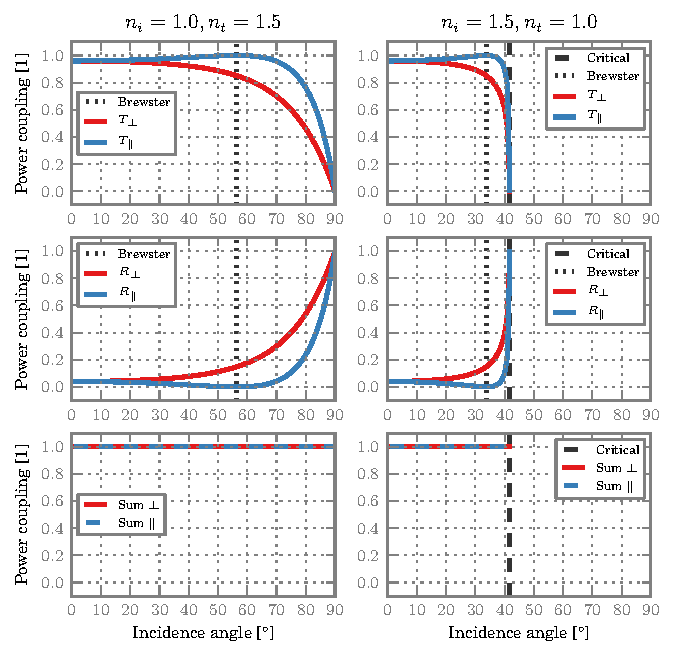
\includegraphics{interface_oblique_verification}
    \caption{Interface oblique, verification}
    \label{fig:interface_oblique_verification}
\end{figure}




%=============================================================================
\clearpage
\subsection{Metallic reflector}
\label{sec:metallic_reflector}
The interface at oblique incidence described in the previous section is limited to dielectrics; or more precisely to materials for which the refractive index is a real number.
Most reflective surfaces inside HIFI are alluminum mirrors.
Alluminum conducts electricity, therefore its refractive index is complex.

When an electromagnetic wave meets a material, its electric field accelerates the electrons of that material.
In return, the accelerating electrons generate an electric field of opposite direction, which creates the reflected wave.
In a conductor, there are free electrons, electrons that are not bound to the atoms of the material.
The free electrons are much more mobile, they can follow the electric field of the incoming wave without being pulled back by their atoms.
As a result, they cancel almost perfectly the electric field of the incoming wave, blocking almost all refraction and generating a quasi-total reflection.

At microwave frequencies, it is customary to consider that metals are perfect reflectors at microwave frequencies.
At normal incidence, the reflection on a metal is very well modeled by a reflection coefficient of~\num{-1}.
Does this still hold at a few terahertz?

As written in~\cref{eq:epsilon_admittivity}, the effect of conductivity~$\sigma'$ of a material is mitigated by the angular frequency~$\omega$:
$\hat{\epsilon} = \epsilon' + i \sigma' / \omega$.
At high frequencies, the electrons cannot accelerate fast enough to cancel the electric field;
as a result, the material becomes more and more transparent, less and less reflective.
Furthermore, the oscillation of the electrons starts lagging behind that of the incoming wave, leading to a noticable phase shift.
Not only does the reflection coefficient get closer to~0, it also gains an imaginary part to represent this phase shift.

The equations of Snell and Fresnel still hold for complex refractive indices
and complex angles of incidence, reflection and refraction.
\Cref{eq:snell_complex} presents Snell's equation with complex angles and indices.
\begin{equation}
    \hat{n}_a \sin \hat{\theta}_a = \hat{n}_b \sin \hat{\theta}_b \label{eq:snell_complex}
\end{equation}

One way to understand complex angles is to consider that rotations are linear transformations.
For example, a rotation of angle~$\hat{\theta}$ around the~$\vect{x}$ axis can be represented by the following matrix
\begin{equation}
    \begin{pmatrix}
        1 & 0 & 0\\
        0 & \cos \hat{\theta} & - \sin \hat{\theta} \\
        0 & \sin \hat{\theta} & \phantom{-}\cos \hat{\theta}
    \end{pmatrix}
\end{equation}
with
\begin{align}
    \cos{\hat{\theta}} &= \frac{\exp(i\hat{\theta}) + \exp(-i\hat{\theta})}{2}
    &
    \sin{\hat{\theta}} &= \frac{\exp(i\hat{\theta}) - \exp(-i\hat{\theta})}{2i}%
    \text{.}
\end{align}
When a complex vector is rotated by a real angle, its components are scaled but the argument of each component is preserved.
When it is rotated by a complex angle, the argument of the components is modified as well.
Complex angles may feel strange at first from a geometrical point of view but are perfectly banal from an algebraic point of view.

One particularity of rotations by complex angles is the following.
Let $\vect{\hat{k}} = \hat{k} \vect{u}$ be a complex vector.
The vector $\vect{u}$ is real and unit and $\hat{k}$ is a complex scalar.
Therefore, the vectors $\vect{k}_r = \Re(\vect{\hat{k}})$ and $\vect{k}_i = \Im(\vect{\hat{k}})$ are collinear.
The rotation by a real angle preserves the collinearity of the real and imaginary parts of a vector.
However, after a rotation by a complex angle, there is no guarantee that the real and imaginary parts of the rotated vector have the same direction.
If $\vect{\hat{k}}$ is a direction of propagation, then the wave is propagating in the direction of the real part of $\vect{\hat{k}}$ but decays in the direction of the imaginary part of $\vect{\hat{k}}$.
When these two directions differ, we say that the wave is inhomogeneous.
Inhomogeneous waves can occur in homogeneous propagation media.
Inhomogeneous waves are not related to anisotropic media either: in an anisotropic medium, there are several real directions of propagation, here there is one real direction and one imaginary direction.

\citeauthor{stratton1941electromagnetic} has worked out the coefficients of reflection and refraction in the case of complex indices in his book \citetitle{stratton1941electromagnetic}~\cite{stratton1941electromagnetic}.
We are not going to rederive them.


%=============================================================================
\clearpage
\subsection{Thin film at normal incidence}
\label{sec:thin_film_at_normal_incidence}


%-----------------------------------------------------------------------------
\subsubsection{Scattering matrix}

Two interfaces separate three regions of space of refractive indices~$n_1$, $n_2$ and~$n_3$ (in most cases, $n_1=n_3$).
Each interface of the film reflects and transmits radiation according to the Fresnel equations for normal incidence~\eqref{eq:fresnel_normal}.
\Cref{fig:thin_film_normal} defines the notations for the reflection and transmission coeffients between the three regions of space.
The propagation between the two interfaces introduces a factor $a$.
\Cref{fig:thin_film_normal_collapsed} is what results of our modeling effort: a single network with two reflections and two transmissions.
\begin{figure}[hbtp]
    \centering
    \input{thin_film_normal.pdf_tex}
    \caption{Thin film at normal incidence.}
    \label{fig:thin_film_normal}
\end{figure}
\begin{figure}[hbtp]
    \centering
    \input{thin_film_normal_collapsed.pdf_tex}
    \caption{Thin film at normal incidence, collapsed.}
    \label{fig:thin_film_normal_collapsed}
\end{figure}

\Crefrange{eq:thin_film_normal_0}{eq:thin_film_normal_2} walk us through the derivation of~$r_{1, 3}$, the reflection coefficient of the thin film seen from the region of refractive index~$n_1$.
\begin{align}
    r_{1,3}
    &= r_{1,2} + t_{1,2}
        \left(
            a r_{2,3} a +
            a r_{2,3} a r_{2,1} a r_{2,3} a +
            \cdots
        \right)
       t_{2,1}
    \label{eq:thin_film_normal_0}
    \\
    r_{1, 3}
    &=
    r_{1, 2} + t_{1, 2} t_{2, 1} a^2r_{2, 3}
        \sum_{i=0}^{\infty} (a^2r_{2,1}r_{2,3})
    \label{eq:thin_film_normal_1}
    \\
    r_{1, 3}
    &=
    r_{1, 2} + t_{1, 2} t_{2, 1} a^2 r_{2, 3}
    \frac{1}{1 - a^2 r_{2, 1} r_{2, 3}}
    \label{eq:thin_film_normal_2}
\end{align}
Likewise, we can derive $r_{3, 1}$, $t_{1, 3}$ and $t_{3, 1}$.
They are given by \crefrange{eq:thin_film_normal_r31}{eq:thin_film_normal_t31},
with \cref{eq:thin_film_normal_r13} being a mere reminder of \cref{eq:thin_film_normal_2}.
\begin{subequations}
    \begin{align}
        r_{1, 3}
        &=
        r_{1, 2} + t_{1, 2} t_{2, 1} a^2 r_{2, 3}
        \frac{1}{1 - a^2 r_{2, 1} r_{2, 3}}
        \label{eq:thin_film_normal_r13}
        \\
        r_{3, 1}
        &=
        r_{3, 2} + t_{3, 2} t_{2, 3} a^2 r_{2, 1}
        \frac{1}{1 - a^2 r_{2, 3} r_{2, 1}}
        \label{eq:thin_film_normal_r31}
        \\
        t_{1, 3}
        &=
        t_{1,2} t_{2,3} a \frac{1}{1 - a^2 r_{2, 3} r_{2, 1}}
        \label{eq:thin_film_normal_t13}
        \\
        t_{3, 1}
        &=
        t_{3,2} t_{2,1} a \frac{1}{1 - a^2 r_{2, 1} r_{2, 3}}
        \label{eq:thin_film_normal_t31}
    \end{align}
\end{subequations}
The parameters $r_{1, 2}$, $t_{1, 2}$, $r_{3, 2}$, $t_{3, 2}$, $r_{2, 1}$, $t_{2, 1}$,
$r_{2, 3}$ and $t_{2, 3}$ are determined by the Fresnel equations for normal incidence~\eqref{eq:fresnel_normal}.
The parameter $a$ is determined by $\exp(-i 2 \pi d n f / c_0)$ according to \cref{eq:net_distance}.
Note that in these four equations, the fraction is the same;
it is sufficient to compute its value once only.



There is one more factor to apply: a compensation for the space taken by the film.
As illustrated in \cref{fig:thin_film_normal_compensation},
the film has a thickness $d_2$ and
its center is located at distances $d_1$ and $d_3$ from other reference points.
The actual length of the medium 1 is not $d_1$ but $d_1 - d_2/2$.
Likewise, the wave travels a distance $d_3 - d_2/2$ in the medium 3.
\begin{figure}[hbtp]
    \centering
    \input{thin_film_normal_compensation.pdf_tex}
    \caption{Thin film at normal incidence, space compensation.}
    \label{fig:thin_film_normal_compensation}
\end{figure}
One way of accounting for this without changing any other network is to add some negative space on each side of the film.
Let $a_1$ and $a_3$ be the effect of these negative spaces.
\Crefrange{eq:negative_space_3}{eq:negative_space_3} apply \cref{eq:net_distance} to the refractive indices $n_1$ and $n_3$ for the negative distance $-d_2/2$.
\begin{subequations}
    \begin{align}
        a_1 &= \exp \Big(-i 2 \pi (-d_2/2) n_1 f / c_0 \Big) \label{eq:negative_space_1}
        \\
        a_3 &= \exp \Big(-i 2 \pi (-d_2/2) n_3 f / c_0 \Big) \label{eq:negative_space_3}
    \end{align}
    \label{eq:negative_space}
\end{subequations}
The reflection on the left side crosses the negative space $a_1$ twice, therefore $r_{1, 3}$ must be multiplied by $a_1^2$.
Likewise, $r_{3, 1}$ must be multiplied by $a_3^2$.
Both transmissions $t_{1, 3}$ and $t_{3, 1}$ go through $a_1$ and $a_3$, therefore they must be multiplied by $a_1 a_3$.
This is summarized with \crefrange{eq:thin_film_normal_compensated_r13}{eq:thin_film_normal_compensated_t31}.
\begin{subequations}
    \begin{align}
        r'_{1, 3} &= a_1^2   \, r_{1, 3} \label{eq:thin_film_normal_compensated_r13} \\
        r'_{3, 1} &= a_3^2   \, r_{3, 1} \label{eq:thin_film_normal_compensated_r31} \\
        t'_{1, 3} &= a_1 a_3 \, t_{1, 3} \label{eq:thin_film_normal_compensated_t13} \\
        t'_{3, 1} &= a_1 a_3 \, t_{3, 1} \label{eq:thin_film_normal_compensated_t31}
    \end{align}
    \label{eq:thin_film_normal_compensated}
\end{subequations}

From there, building the scattering matrix of the thin film is straightforward.
If we name $I_3$ the 3--by--3 identity matrix,
then the Jones matrices  \crefrange{eq:thin_film_normal_s11}{eq:thin_film_normal_s22}
are the elements of the scattering matrix.
\begin{subequations}
    \begin{align}
        S_{1, 1} &= r'_{1, 3} I_3 \label{eq:thin_film_normal_s11} \\
        S_{1, 2} &= t'_{3, 1} I_3 \label{eq:thin_film_normal_s12} \\
        S_{2, 1} &= t'_{1, 3} I_3 \label{eq:thin_film_normal_s21} \\
        S_{2, 2} &= r'_{3, 1} I_3 \label{eq:thin_film_normal_s22}
    \end{align}
    \label{eq:thin_film_normal_sij}
\end{subequations}
If necessary, each of these Jones matrices can be adapted to account for the orientation of the thin film;
see~\vref{sec:rotating_jones_matrices}.

%-----------------------------------------------------------------------------
\subsubsection{Verification}
We have derived a model that treats a thin film as a single two-port network.
It should yield the same results as a system of three networks
(interface--space--interface).
In this section, we verify this numerically.

\Cref{fig:thin_film_normal_verification_principle} defines the distances and refractive indices used in this section.
It also illustrates the two systems that we wish to compare:
\begin{itemize}
    \item one system made of three networks (two spaces, one thin film), that we call ``thin film model'';
    \item one system made of five networks (three spaces and two interfaces), that we call ``interfaces model''.
\end{itemize}
\begin{figure}[hbtp]
    \centering
    \input{thin_film_normal_verification_principle.pdf_tex}
    \caption{Thin film at normal incidence, verification, principle.}
    \label{fig:thin_film_normal_verification_principle}
\end{figure}

\Cref{fig:thin_film_normal_verification} presents the result of both models for
$n_1=1.00$, $n_2=1.75$, $n_3=1.50$,
$d_1=\SI{1}{\meter}$, $d_2=\SI{10}{\micro\meter}$ and $d_3=\SI{1}{\meter}$.
The source is on the leftmost port.
The ``Reflected'' plot corresponds to the output of that leftmost port.
The ``Transmitted'' plot corresponds to the output of the rightmost port.
\begin{figure}[hbtp]
    \centering
    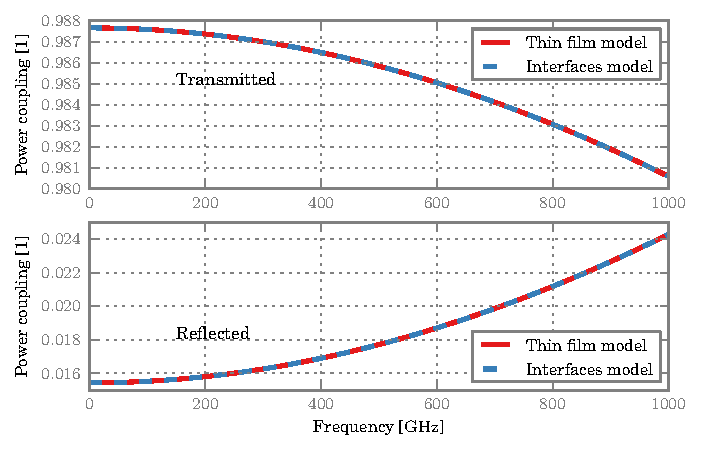
\includegraphics{thin_film_normal_verification.pdf}
    \caption{Thin film at normal incidence, verification.}
    \label{fig:thin_film_normal_verification}
\end{figure}

Both models agree within numerical noise.
The advantage of the thin film model over the other is that a thin film is represented by a single network.
This is easier for the programmer and faster for the computer.

The curvature of the power coupling displayed in \cref{fig:thin_film_normal_verification} comes from standing waves inside the thin film.
\Cref{eq:cavity_period} predicts a period of $F = c_0 / (2 n_2 d_2) \approx \SI{9993}{\tera\hertz}$.
Thin cavities (here \SI{10}{\micro\meter}) create standing wave patterns with very large periods.



%=============================================================================
\subsection{Thin film at oblique incidence}
\label{sec:thin_film_at_oblique_incidence}

A thin film at oblique incidence forms a four-port network.
\Cref{fig:thin_film_oblique} defines the geometry and the port-numbering that we use.
\begin{figure}[hbtp]
    \centering
    \missingfigure{Thin film oblique}
    \caption{Thin film at oblique incidence}
    \label{fig:thin_film_oblique}
\end{figure}

When deriving the scattering matrix of a thin film at normal incidence in \cref{sec:thin_film_at_normal_incidence}, we allowed for three refractive indices: one for the film itself and one for each propagation medium on each side of the film.
This was a generalization that came at barely no cost because the geometry was simple.
In the case of a thin film at oblique incidence, we assume that the propagation medium on each side of the thin film has the same refractive index.
This is, after all, the most common case;
for example, a beam splitter placed in vacuum has vacuum on both sides.
If that constraint is too strong, it is always possible to model that thin film with three networks by using two interfaces and a distance (see sections~\ref{sec:generic_networks_distance} and \ref{sec:interface_at_oblique_incidence}).

%-----------------------------------------------------------------------------
\subsubsection{Geometry}
\label{sec:thin_film_geometry}
We need to determine the angle of incidence, the parallel and perpendicular decomposition matrices and the various rotation matrices.

It is assumed that we know the orientation of the thin film via its normal $n$ and the direction of propagation $k_1$ of the wave incident to the port 1.

From $n$ and $k_1$, we can apply \cref{eq:angle_from_dot_product} to compute the angle of incidence~$\theta_a$.
We get the refracted angle~$\theta_b$ from $\theta_a$ with \cref{eq:snell_thetab}.

We use \cref{eq:normal_to_plane_of_incidence} to retreive the normal to the plane-of-incidence $u$.

From the normal $u$ to the plane-of-incidence
and \cref{eq:para_perp_decomposition_matrix},
we determine the parallel and perpendicular projection matrices,
$M_\parallel$ and $M_\perp$.

From $u$ and
equations~\eqref{eq:quaternion_rotation_around_axis}
and \eqref{eq:quaternion_to_rotation_matrix}, we can compute the rotation matrices to apply to the Jones matrices and the direction of propagation.
The angles that we need are listed in \cref{eq:thin_film_angles}.
\begin{equation}
    \begin{aligned}
        \theta_{1 \leftarrow 2} &= 2 \theta_a
        &
        \theta_{2 \leftarrow 1} &= -2 \theta_a
        \\
        \theta_{3 \leftarrow 4} &= 2 \theta_a
        &
        \theta_{4 \leftarrow 3} &= -2 \theta_a
        \\
        \theta_{4 \leftarrow 1} &= -2 \theta_a
    \end{aligned}
    \label{eq:thin_film_angles}
\end{equation}
These angles $\theta_{i \leftarrow j}$ have corresponding rotation matrices $R^{i \leftarrow j}$.
We can already determine the directions of propagation of the waves exiting the thin film with \cref{eq:thin_film_propagation_rotation_ki}.
\begin{subequations}
    \begin{align}
        k_2 &= -R^{2 \leftarrow 1} k_1
        \label{eq:thin_film_propagation_rotation_k2}\\
        k_3 &= k_1
        \label{eq:thin_film_propagation_rotation_k3}\\
        k_4 &= R^{4 \leftarrow 1} k_1
        \label{eq:thin_film_propagation_rotation_k4}
    \end{align}
    \label{eq:thin_film_propagation_rotation_ki}
\end{subequations}

%-----------------------------------------------------------------------------
\subsubsection{Reflection and transmission coefficients}
In the previous section (\cref{sec:thin_film_geometry}) we have determined the decomposition and rotation matrices that are needed to compute the reflection and refraction coefficients of a thin film at oblique incidence.
We also have the angle of incidence and the refracted angle.

We want to apply the Fresnel equations for oblique incidence \eqref{eq:fresnel_oblique} twice:
once for entering the thin film, and once for leaving it.
\begin{itemize}
    \item 
$r_{\parallel a}$, $r_{\perp a}$, $t_{\parallel a}$ and $t_{\perp a}$ correspond to entering the film.
They are derived from \cref{eq:fresnel_oblique} with
$\theta_i = \theta_a$, $\theta_t = \theta_b$,
$n_i = n_a$ and $n_t = n_b$.
    \item
$r_{\parallel b}$, $r_{\perp b}$, $t_{\parallel b}$ and $t_{\perp b}$ correspond to exiting the film.
They are derived from \cref{eq:fresnel_oblique} with
$\theta_i = \theta_b$, $\theta_t = \theta_a$,
$n_i = n_b$ and $n_t = n_a$.
\end{itemize}

The pathlength $l_b$ inside the film is not equal to the thickness $d$ of the thin film because $\theta_b \ne 0$, as described by \cref{eq:thin_film_oblique_pathlength}.
\begin{equation}
    l_b = \frac{d}{\cos \theta_b}
    \label{eq:thin_film_oblique_pathlength}
\end{equation}
To this distance $l_b$ corresponds a gain $a_b$ that we derive from \cref{eq:net_distance}.
Its expression is given for $l_b$ in \cref{eq:thin_film_distance}.
\begin{equation}
    a_b = \exp(-2i \pi l_b n_b f / c_0)
    \label{eq:thin_film_distance}
\end{equation}
This pathlength $l_b$ must be compensated for.
Indeed, the pathlength $l_b$ inside the film replaces a pathlength $l_a$ in the material $n_a$.
\begin{equation}
    l_a = \frac{d}{\cos \theta_a}
    \label{eq:thin_film_oblique_pathlength_compensation}
\end{equation}
\begin{equation}
    a_a = \exp(-2i \pi (-l_a) n_a f / c_0)
    \label{eq:thin_film_distance_compensation}
\end{equation}

What follows is similar to what we did for the thin film at normal incidence.
One difference is that do it twice, one for the parallel parameters and one for the perpendicular parameters.
Another difference is that we have two and not three refractive indices, which gives a few simplifications.
\begin{subequations}
    \begin{align}
        t_\parallel
        &=
        a_a \,
        t_{\parallel a} \, t_{\parallel b} \, a_b
        \frac{1}{
            1 - (r_{\parallel b} \, a_b)^2
        }
        \\
        t_\perp
        &=
        a_a \,
        t_{\perp a} \, t_{\perp b} \, a_b
        \frac{1}{
            1 - (r_{\perp b} \, a_b)^2
        }
        \\
        r_\parallel
        &=
        a_a \,
        r_{\parallel a} + r_{\parallel b} \, a_b \, t_\parallel
        \\
        r_\perp
        &=
        a_a \,
        r_{\perp a} + r_{\perp b} \, a_b \, t_\perp
    \end{align}
\end{subequations}

\subsubsection{Scattering matrix}
Because we use one refractive index only outside the film, the transmitted waves are not rotated.
\begin{equation}
    S_{1, 3} =
    S_{2, 4} =
    S_{3, 1} =
    S_{4, 2} =
    t_\parallel M_\parallel
    +
    t_\perp M_\perp
    \label{eq:thin_film_s_t}
\end{equation}

The reflections, however, require some rotations.
\begin{subequations}
    \begin{align}
        S_{1, 2} = R^{1 \leftarrow 2} (r_\parallel M_\parallel + r_\perp M_\perp) \\
        S_{2, 1} = R^{2 \leftarrow 1} (r_\parallel M_\parallel + r_\perp M_\perp) \\
        S_{3, 4} = R^{3 \leftarrow 4} (r_\parallel M_\parallel + r_\perp M_\perp) \\
        S_{4, 3} = R^{4 \leftarrow 3} (r_\parallel M_\parallel + r_\perp M_\perp)
    \end{align}
    \label{eq:thin_film_s_r}
\end{subequations}

Finally, many paths are forbidden.
\begin{equation}
    S_{1, 1} = S_{1, 4} = S_{2, 2} = S_{2, 3} =
    S_{3, 2} = S_{3, 3} = S_{4, 1} = S_{4, 4} = 
    \begin{pmatrix}
        0&0&0\\0&0&0\\0&0&0
    \end{pmatrix}
    \label{eq:thin_film_s_zero}
\end{equation}

\Crefrange{eq:thin_film_s_t}{eq:thin_film_s_zero} define the scattering parameters of the 4--by--4 scattering matrix of a thin film at oblique incidence.


\subsubsection{Verification}
Our model for a thin film at oblique incidence should provide exactly the same result as two interfaces and a distance.
The goal of the thin film model is to provide convenience, not introduce new physics.
\Cref{fig:thin_film_oblique_verification} illustrates a comparison between these two ways of modeling a thin film.
The angle of incidence is~\SI{45}{\degree}.
The film is~\SI{10}{\micro\meter} thick.
The refractive indices are 1.0 outside the film and 1.5 in the film.
The thickness of the film creates a cavity and therefore a standing wave.
This standing wave is responsable for the frequency-dependance of the reflected and transmitted power seen on \cref{fig:thin_film_oblique_verification}.

\begin{figure}[hbtp]
    \centering
    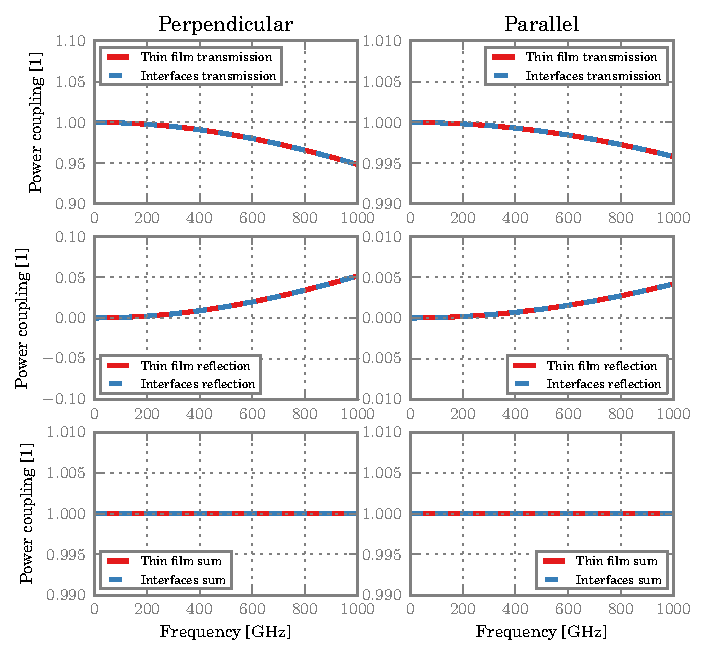
\includegraphics{thin_film_oblique_verification}
    \caption{Thin film at oblique incidence, verification}
    \label{fig:thin_film_oblique_verification}
\end{figure}

The top row of \cref{fig:thin_film_oblique_verification} shows the transmitted power, the middle row shows the reflected power, and the bottom row shows the sum of the two.
That last row shows that energy is conserved: the power that is not transmitted is reflected.

The left column shows the transmitted, reflected and total power coupling for the perpendicular polarization.
The right column corresponds to the parallel polarization.
Note that the vertical-axes differ for the two polarizations: the standing wave has an effect about ten times stronger on the perpendicular polarization.

Finally, each plot shows two overlapped curves.
The red curve corresponds to the model derived in this section with which the thin film is seen as a single network.
The blue curve corresponds to a model made of two interfaces and a distance.

As expected, both models agree within numerical noise.
This agreement does not only happen in power, but also in field.
The phasor predicted by both methods agree within $10^{-10}$: the magnitude of the difference of the phasors is smaller than $10^{-10}$ for frequencies of the order of \SI{1}{\tera\hertz}.  \todo{Should I put a pic?}



%=============================================================================
\subsection{Wire grid polarizer}
\todo{Check k omega convention}
In their paper from \citeyear{houde_2001} \citetitle{houde_2001}, \textcite{houde_2001} present a set of equations that approximate the electric field at any point near a wire grid polarizer.
The incident wave is assumed plane, the surrounding propagation medium is assumed homogeneous and isotropic, and the wires are assumed to be free floating (no dielectric substrate) and to have a cylindrical section.

\subsubsection{Geometry}
The article of \citeauthor{houde_2001} \cite{houde_2001} defines the following rest reference frame for the grid: wires in the $\vect{x}\vect{y}$ plane, wires along $\vect{x}$.
Its normal, at rest, is therefore the $\vect{z}$ axis.

If $R$ is the rotation matrix that move the grid from its rest attitude to its useful attitude, then the normal of the grid is $\vect{n}=R \vect{z}$.

The grid is a four port network.
$\vect{k}_1$,  is the direction of propagation of the wave indident to the port 1.
We can derive the direction of propagation of the wave incident to the three other ports easily.
The law of reflection states that $\vect{k}_1$, $\vect{k}_2$ and $\vect{n}$ are coplanar and that the directed angle between $\vect{k}_1$ and $\vect{n}$ equals that between $\vect{n}$ and $\vect{k}_2$.
Therefore, one way of deriving $\vect{k}_2$ is to rotate $\vect{k}_1$ by \SI{180}{\degree} around $\vect{n}$.
Then, $\vect{k}_3=-\vect{k}_1$ and $\vect{k}_4=-\vect{k_2}$.

\subsubsection{Reflection and transmission coefficients}
The set of equations that interest us here are the equations numbered 23 to 35, 62 and 63 in the article of \citeauthor{houde_2001} \cite{houde_2001}, which we copied here for convenience.
The first two equations, \eqref{eq:grid_current_linear} and \eqref{eq:grid_current_circular}, describe the electric current in the wires.
$K^x$ corresponds to a linear current and $K^\theta$ to a circular current.
In the first case, electrons move along the length of the wire; in the other, they rotate around the axis of the wire.
\begin{align}
    K^x &= \frac{E_0}{F} \cdot \alpha' \frac{N_x}{\Delta_x}
    \label{eq:grid_current_linear}
    \\
    K^\theta &= (-j) \frac{E_0}{F} \cdot (\gamma' \beta - \beta' \gamma) \frac{N_\theta}{\Delta_\theta}
    \label{eq:grid_current_circular}
\end{align}
with
\begin{align}
    N_x
    &=
    1 - j \frac{Z_s}{Z_0} \frac{ka}{2}
    \\
    \Delta_x
    &=
    (1 - \alpha^2) S_1 - j \frac{Z_s}{Z_0} \sqrt{1 - \alpha^2}H_1^{(2)} (k'a)
    \\
    N_\theta
    &=
    1 + j \frac{Z_s}{Z_0} \frac{2}{ka}
    \\
    \Delta_\theta
    &=
    \sqrt{1 - \alpha^2} H_1^{(2)} (k'a) + j \frac{Z_s}{Z_0} (1 - \alpha^2) S_1
\end{align}
and
\begin{equation}
    S_1 = H_0^{(2)} (k'a) + 2
    \sum_{n=1}^\infty
    H_0^{(2)}(k'nd) \cos (k \beta nd)
    \text{.}
    \label{eq:infinite_hankel}
\end{equation}
The following equations use the previous definitions.
They describe the reflected and transmitted fields in three dimensions for a grid in the $xy$-plane, wires along~$x$.
\begin{align}
    R^x
    &=
    -\frac{F}{E_0}
    \frac{\lambda}{\pi d}
    \frac{1 - \alpha^2}{\gamma} K^x
    \label{eq:houde_Rx}
    \\
    R^y
    &=
    \phantom{-}
    \frac{F}{E_0}
    \frac{\lambda}{\pi d}
    \left[
        \frac{\alpha \beta}{\gamma} K^x
        -
        j \frac{ka}{2} K^\theta
    \right]
    \\
    R^z
    &=
    -\frac{F}{E_0}
    \frac{\lambda}{\pi d}
    \left[
       \alpha K^x
       +
       j \frac{\beta}{\gamma} \frac{ka}{2} K^\theta
    \right]
    \\
    T^x &= \alpha' + R^x
    \\
    T^y
    &=
    \beta' +
    \frac{F}{E_0}
    \frac{\lambda}{\pi d}
    \left[
        \frac{\alpha \beta}{\gamma} K^x + j \frac{ka}{2} K^\theta
    \right]
    \\
    T^z
    &=
    \gamma' +
    \frac{F}{E_0}
    \frac{\lambda}{\pi d}
    \left[
        \alpha K^x - j \frac{\beta}{\gamma} \frac{ka}{2} K^\theta
    \right]
\end{align}
Note that Houde calls these $R$ and $T$ ``reflection'' and ``transmission coefficient'', something they are not quite since they contain $\alpha'$, $\beta'$ and $\gamma'$, corresponding to the amplitude of the incoming electric field in the three dimensions.
These amplitudes have to be factored out if we want to really speak about reflection or transmission coefficients.

When implementing these equations, some simplifications are obvious.
For example, $\frac{E_0}{F}$ inside $K^x$ and $K^\theta$ cancels $\frac{F}{E_0}$ in $R$ and $T$;
the complex unit $j$ within $K^\theta$ combines with $j$ in $R$ and $T$ to become -1.

In these equations, $\alpha'$, $\beta'$ and $\gamma'$ are the three components of the direction of the incident electric field, satisfying $\alpha'^2 + \beta'^2 + \gamma'^2 = 1$.
That condition seems to apply only to real numbers, restricting the use of this grid model to waves that are linearly polarized (their three components are in phase).
However, there is no such limitation in the model.
Indeed, the authors define the incident electric field as $(e_x, e_y, e_z) = E_0(\alpha', \beta', \gamma')$.
The amplitude $E_0$ can be complex and it seems that its phase has to be shared among the three components.
However, when we rewrite the equations to fit in a matrix, we will notice that the real parameters are not $\alpha'$, $\beta'$, $\gamma'$ and $E_0$, but $e_x$, $e_y$ and $e_z$ directly, which are all independant.
In that case, each of them is free to have its own phase and the model also applies to elliptically polarized waves.


In order to rewrite these equations in a matrix form that depends on $e_x$, $e_y$ and $e_z$, one needs to split each coefficient of transmission and reflection into three, like this:
\begin{equation}
    e_{rx} = R^{xx} e_x + R^{xy} e_y + R^{xz} e_z
\end{equation}
so that we can write
\begin{align}
    e_r &= R e_i \\
    e_r &=
    \begin{pmatrix}
        R_{xx} & R_{xy} & R_{xz} \\
        R_{yx} & R_{yy} & R_{yz} \\
        R_{zx} & R_{zy} & R_{zz}
    \end{pmatrix}
    e_i
\end{align}
for the reflection $R$ and a similar equation for the transmission $e_t = T e_i$.
I start with $R_x$ defined in \cref{eq:houde_Rx} to get $R_{xx}$, $R_{xy}$ and $R_{xz}$.
\begin{align*}
    e_{rx} &= R^x E_0
    \\
           &= -\frac{F}{E_0}
              \frac{\lambda}{\pi d}
              \frac{1-\alpha^2}{\gamma}
              K^x
              E_0
    \\
           &= -\cancel{\frac{F}{E_0}}
              \frac{\lambda}{\pi d}
              \frac{1-\alpha^2}{\gamma}
              \cancel{\frac{E_0}{F}}
              \frac{N_x}{\Delta_x}
              \underbrace{
                  \alpha'
                  E_0
              }_{e_{ix}}
    \\
           &= -\frac{\lambda}{\pi d}
              \frac{1-\alpha^2}{\gamma}
              \frac{N_x}{\Delta_x}
              e_{ix}
\end{align*}
By identification, we find these values for $R_{xx}$, $R_{xy}$ and $R_{xz}$.
\begin{equation}
    \left\lbrace
    \begin{aligned}
        R_{xx} &= -\frac{\lambda}{\pi d}
                  \frac{N_x}{\Delta_x}
                  \frac{1-\alpha^2}{\gamma}
        \\
        R_{xy} &= 0
        \\
        R_{xz} &= 0
    \end{aligned}
    \right.
\end{equation}
Let us continue with $R_y$.
\begin{align*}
    e_{ry}
    &= R^y E_0
    \\
    &= \frac{F}{E_0}
       \frac{\lambda}{\pi d}
       \left[
           \frac{\alpha \beta}{\gamma}
           K^x
           -
           j
           \frac{ka}{2}
           K^\theta           
       \right]
       E_0
    \\
    &= \cancel{\frac{F}{E_0}}
       \frac{\lambda}{\pi d}
       \left[
           \frac{\alpha \beta}{\gamma}
           \cancel{\frac{E_0}{F}}
           \frac{N_x}{\Delta_x}
           \alpha'
           -
           j
           \frac{ka}{2}
           (-j)
           \cancel{\frac{E_0}{F}}
           \frac{N_\theta}{\Delta_\theta}
           (\gamma' \beta - \beta' \gamma)           
       \right]
       E_0
    \\
    &= \frac{\lambda}{\pi d}
       \left[
           \frac{\alpha \beta}{\gamma}
           \frac{N_x}{\Delta_x}
           \alpha'
           +
           \frac{ka}{2}
           \frac{N_\theta}{\Delta_\theta}
           \gamma
           \beta'
           -
           \frac{ka}{2}
           \frac{N_\theta}{\Delta_\theta}
           \beta
           \gamma'
       \right]
       E_0
    \\
    &= \frac{\lambda}{\pi d}
       \frac{\alpha \beta}{\gamma}
       \frac{N_x}{\Delta_x}
       \underbrace{E_0 \alpha'}_{e_{ix}}
       +
       \frac{\lambda}{\pi d}
       \frac{ka}{2}
       \frac{N_\theta}{\Delta_\theta}
       \gamma
       \underbrace{E_0 \beta'}_{e_{iy}}
       -
       \frac{\lambda}{\pi d}
       \frac{ka}{2}
       \frac{N_\theta}{\Delta_\theta}
       \beta
       \underbrace{E_0 \gamma'}_{e_{iz}}
\end{align*}
\begin{equation}
    \left\lbrace
    \begin{aligned}
        R_{yx}
        &=
        \phantom{-}
        \frac{\lambda}{\pi d}
        \frac{N_x}{\Delta_x}
        \frac{\alpha \beta}{\gamma}
        \\
        R_{yy}
        &=
        \phantom{-}
        \frac{\lambda}{\pi d}
        \frac{N_\theta}{\Delta_\theta}
        \frac{ka}{2}
        \gamma
        \\
        R_{yz}
        &=
        -
        \frac{\lambda}{\pi d}
        \frac{N_\theta}{\Delta_\theta}
        \frac{ka}{2}
        \beta
    \end{aligned}
    \right.
\end{equation}
Same thing for $R_z$.
\begin{align*}
    e_{rz} &= R^z E_0
    \\
    &=
    -
    \frac{F}{E_0}
    \frac{\lambda}{\pi d}
    \left[
        \alpha K^x
        +
        j
        \frac{\beta}{\gamma}
        \frac{ka}{2}
        k^\theta
    \right]
    E_0
    \\
    &=
    -
    \cancel{\frac{F}{E_0}}
    \frac{\lambda}{\pi d}
    \left[
        \alpha
        \cancel{\frac{E_0}{F}}
        \frac{N_x}{\Delta_x}
        \alpha'
        +
        j
        \frac{\beta}{\gamma}
        \frac{ka}{2}
        (-j)
        \cancel{\frac{E_0}{F}}
        (\gamma' \beta - \beta' \gamma)
        \frac{N_\theta}{\Delta_\theta}
    \right]
    E_0
    \\
    &=
    -
    \frac{\lambda}{\pi d}
    \alpha
    \frac{N_x}{\Delta_x}
    \underbrace{E_0 \alpha'}_{e_{ix}}
    +
    \frac{\lambda}{\pi d}
    \frac{\beta}{\gamma}
    \frac{ka}{2}
    \frac{N_\theta}{\Delta_\theta}
    \gamma
    \underbrace{E_0 \beta'}_{e_{iy}}
    -
    \frac{\lambda}{\pi d}
    \frac{\beta}{\gamma}
    \frac{ka}{2}
    \frac{N_\theta}{\Delta_\theta}
    \beta
    \underbrace{E_0 \gamma'}_{e_{iz}}
\end{align*}
\begin{equation}
    \left\lbrace
    \begin{aligned}
        R_{zx}
        &=
        -
        \frac{\lambda}{\pi d}
        \frac{N_x}{\Delta_x}
        \alpha
        \\
        R_{zy}
        &=
        \phantom{-}
        \frac{\lambda}{\pi d}
        \frac{N_\theta}{\Delta_\theta}
        \frac{ka}{2}
        \beta
        \\
        R_{zz}
        &=
        -
        \frac{\lambda}{\pi d}
        \frac{N_\theta}{\Delta_\theta}
        \frac{ka}{2}
        \frac{\beta^2}{\gamma}
    \end{aligned}
    \right.
\end{equation}
We have the reflection matrix.
Now, we compute the transmission matrix.
\begin{align*}
    e_{tx} &= T^x E_0
    \\
    &= (\alpha' + R^x) E_0
    \\
    &= \underbrace{\alpha' E_0}_{e_{ix}}
       -
       \frac{\lambda}{\pi d}
       \frac{1 - \alpha^2}{\gamma}
       \frac{N_x}{\Delta_x}
       \underbrace{\alpha' E_0}_{e_{ix}}
    \\
    &= \left(
           1
           -
           \frac{\lambda}{\pi d}
           \frac{1 - \alpha^2}{\gamma}
           \frac{N_x}{\Delta_x}
       \right)
       e_{ix}
\end{align*}
\begin{equation}
    \left\lbrace
    \begin{aligned}
        T_{xx}
        &= 1
           -
           \frac{\lambda}{\pi d}
           \frac{N_x}{\Delta_x}
           \frac{1 - \alpha^2}{\gamma}
        \\
        T_{xy} &= 0
        \\
        T_{xz} &= 0
    \end{aligned}
    \right.
\end{equation}

\begin{align*}
    e_{ty} &= T^y E_0
    \\
    &=
    \left(
        \beta'
        +
        \frac{F}{E_0}
        \frac{\lambda}{\pi d}
        \left[
            \frac{\alpha \beta}{\gamma}
            K^x
            +
            j
            \frac{ka}{2}
            K^\theta
        \right]
    \right)
    E_0
    \\
    &=
    \left(
        \beta'
        +
        \cancel{\frac{F}{E_0}}
        \frac{\lambda}{\pi d}
        \left[
            \frac{\alpha \beta}{\gamma}
            \cancel{\frac{E_0}{F}}
            \frac{N_x}{\Delta_x}
            \alpha'
            +
            j
            \frac{ka}{2}
            (-j)
            \cancel{\frac{E_0}{F}}
            \frac{N_\theta}{\Delta_\theta}
            (\gamma' \beta - \beta' \gamma)
        \right]
    \right)
    E_0
    \\
    &=
    \left(
        \beta'
        +
        \frac{\lambda}{\pi d}
        \frac{\alpha \beta}{\gamma}
        \frac{N_x}{\Delta_x}
        \alpha'
        -
        \frac{\lambda}{\pi d}
        \frac{ka}{2}
        \frac{N_\theta}{\Delta_\theta}
        \gamma
        \beta'
        +
        \frac{\lambda}{\pi d}
        \frac{ka}{2}
        \frac{N_\theta}{\Delta_\theta}
        \beta
        \gamma'
    \right)
    E_0
    \\
    &=
    \frac{\lambda}{\pi d}
    \frac{\alpha \beta}{\gamma}
    \frac{N_x}{\Delta_x}
    \underbrace{E_0 \alpha'}_{e_{ix}}
    +
    \left(
        1
        -
        \frac{\lambda}{\pi d}
        \frac{ka}{2}
        \frac{N_\theta}{\Delta_\theta}
        \gamma
    \right)
    \underbrace{E_0 \beta'}_{e_{iy}}
    +
    \frac{\lambda}{\pi d}
    \frac{ka}{2}
    \frac{N_\theta}{\Delta_\theta}
    \beta
    \underbrace{E_0 \gamma'}_{e_{iz}}
\end{align*}
\begin{equation}
    \left\lbrace
    \begin{aligned}
        T_{yx}
        &= \frac{\lambda}{\pi d}
           \frac{N_x}{\Delta_x}
           \frac{\alpha \beta}{\gamma}
        \\
        T_{yy}
        &= 1
           -
           \frac{\lambda}{\pi d}
           \frac{N_\theta}{\Delta_\theta}
           \frac{ka}{2}
           \gamma
        \\
        T_{yz}
        &= \frac{\lambda}{\pi d}
           \frac{N_\theta}{\Delta_\theta}
           \frac{ka}{2}
           \beta
    \end{aligned}
    \right.
\end{equation}

\begin{align*}
    e_{tz} &= T^z E_0
    \\
    &=
    \left(
        \gamma' +
        \frac{F}{E_0}
        \frac{\lambda}{\pi d}
        \left[
            \alpha K^x - j \frac{\beta}{\gamma} \frac{ka}{2} K^\theta
        \right]
    \right)
    E_0
    \\
    &=
    \left(
        \gamma' +
        \cancel{\frac{F}{E_0}}
        \frac{\lambda}{\pi d}
        \left[
            \alpha
            \cancel{\frac{E_0}{F_0}}
            \frac{N_x}{\Delta_x}
            \alpha'
            -
            j
            \frac{\beta}{\gamma}
            \frac{ka}{2}
            (-j)
            \cancel{\frac{E_0}{F}}
            \frac{N_\theta}{\Delta_\theta}
            (\gamma' \beta - \beta' \gamma)
        \right]
    \right)
    E_0
    \\
    &=
    \left(
        \gamma' +
        \frac{\lambda}{\pi d}
        \left[
            \alpha
            \frac{N_x}{\Delta_x}
            \alpha'
            +
            \frac{\beta}{\gamma}
            \frac{ka}{2}
            \frac{N_\theta}{\Delta_\theta}
            \gamma
            \beta'
            -
            \frac{\beta}{\gamma}
            \frac{ka}{2}
            \frac{N_\theta}{\Delta_\theta}
            \beta
            \gamma'
        \right]
    \right)
    E_0
    \\
    &=
    \frac{\lambda}{\pi d}
    \alpha
    \frac{N_x}{\Delta_x}
    \underbrace{E_0 \alpha'}_{e_{ix}}
    +
    \frac{\lambda}{\pi d}
    \frac{\beta}{\gamma}
    \frac{ka}{2}
    \frac{N_\theta}{\Delta_\theta}
    \gamma
    \underbrace{E_0 \beta'}_{e_{iy}}
    +
    \left(
        1
        -
        \frac{\lambda}{\pi d}
        \frac{\beta}{\gamma}
        \frac{ka}{2}
        \frac{N_\theta}{\Delta_\theta}
        \beta
    \right)
    \underbrace{E_0 \gamma'}_{e_{iz}}
\end{align*}
\begin{equation}
    \left\lbrace
    \begin{aligned}
        T_{zx}
        &= \frac{\lambda}{\pi d}
           \frac{N_x}{\Delta_x}
           \alpha
        \\
        T_{zy}
        &= \frac{\lambda}{\pi d}
           \frac{N_\theta}{\Delta_\theta}
           \frac{ka}{2}
           \frac{\beta}{\gamma}
           \gamma
        \\
        T_{zz}
        &= 1
           -
           \frac{\lambda}{\pi d}
           \frac{N_\theta}{\Delta_\theta}
           \frac{ka}{2}
           \frac{\beta}{\gamma}
           \beta
    \end{aligned}
    \right.
\end{equation}

Another simplification:
\begin{equation}
    k = 2\pi / \lambda
    \quad \Rightarrow \quad
    \frac{\lambda}{\pi d} \frac{ka}{2}
    =
    \frac{\lambda}{\pi d} \frac{2\pi a}{2\lambda}
    =
    \frac{a}{d}
\end{equation}

\begin{equation}
    R =
    \begin{pmatrix}
        -\frac{\lambda}{\pi d}
        \frac{N_x}{\Delta_x}
        \frac{1 - \alpha^2}{\gamma}
        &
        0
        &
        0
        \\
        \frac{\lambda}{\pi d}
        \frac{N_x}{\Delta_x}
        \frac{\alpha \beta}{\gamma}
        &
        \frac{\lambda}{\pi d}
        \frac{N_\theta}{\Delta_\theta}
        \frac{ka}{2}
        \gamma
        &
        -
        \frac{a}{d}
        \frac{N_\theta}{\Delta_\theta}
        \beta
        \\
        -
        \frac{\lambda}{\pi d}
        \frac{N_x}{\Delta_x}
        \alpha
        &
        \frac{a}{d}
        \frac{N_\theta}{\Delta_\theta}
        \beta
        &
        -
        \frac{a}{d}
        \frac{N_\theta}{\Delta_\theta}
        \frac{\beta^2}{\gamma}
    \end{pmatrix}
\end{equation}
\begin{equation}
    T =
    \begin{pmatrix}
        1 -
        \frac{\lambda}{\pi d}
        \frac{N_x}{\Delta_x}
        \frac{1 - \alpha^2}{\gamma}
        &
        0
        &
        0
        \\
        \frac{\lambda}{\pi d}
        \frac{N_x}{\Delta_x}
        \frac{\alpha \beta}{\gamma}
        &
        1 -
        \frac{a}{d}
        \frac{N_\theta}{\Delta_\theta}
        \gamma
        &
        \frac{a}{d}
        \frac{N_\theta}{\Delta_\theta}
        \beta
        \\
        \frac{\lambda}{\pi d}
        \frac{N_x}{\Delta_x}
        \alpha
        &
        \frac{a}{d}
        \frac{N_\theta}{\Delta_\theta}
        \beta
        &
        1 -
        \frac{a}{d}
        \frac{N_\theta}{\Delta_\theta}
        \frac{\beta^2}{\gamma}
    \end{pmatrix}
\end{equation}
These reflection and transmission matrices are Jones matrices.
The parameters are the radius $a$ of the wires,
the distance $d$ between the wires,
the conductivity $\sigma$ of the wires,
the frequency $f$ of the wave and
the direction of propagation $\vect{k_1}=(\alpha, \beta, \gamma)$.
We could consider the impedance of the surrounding medium as an additional parameter instead of using that of vacuum, but we did not need that.

\subsubsection{Scattering matrices}
The reflection and transmission matrices defined above are Jones matrices.
But before, we must apply rotation matrices to them in order to account for the arbitrary orientation of the grid.
Indeed, these Jones matrices are valid for grid lying in the $(x, y)$ plane, with the wires along $x$.






%#############################################################################

\section{Simple systems}
\label{sec:simple_systems}

The idea is to show that it works and makes sense.



%=============================================================================

\subsection{The simplest cavity}
\label{sec:the_simplest_cavity}

\Cref{fig:simple_cavity_principle} illustrates how three networks can represent a simple cavity: two interfaces separated by some space.
The three networks all have two ports numbered according to \cref{fig:simple_cavity_principle}.
Ports 2 and 3 are coupled, and so are ports 4 and 5.
Ports 1 and 6 are open to the outside world.

\begin{figure}[hbtp]
    \centering
    \input{simple_cavity_principle.pdf_tex}
    \caption{Simple cavity, principle.}
    \caption*{
        Two reflective surfaces facing each other form a cavity.
        Here, the surfaces are defined by the interfaces (vertical dotted lines)
        between regions of space of different refractive indices $n_1$ and $n_2$.
        According to the Fresnel equations~\eqref{eq:fresnel_normal}, these interfaces
        reflect and transmit part of the incident radiation (black arrows).
        As a result, a standing wave is formed inside the cavity.
        That standing wave is the superposition of an infinity of traveling waves
        interfering with each other.
        We can model such a system with three two-port networks:
        one for each interface and one for the space between them.
        The numbers 1 to~6 are our arbitrary labels for the ports.
    }
    \label{fig:simple_cavity_principle}
\end{figure}
\begin{figure}[hbtp]
    \centering
    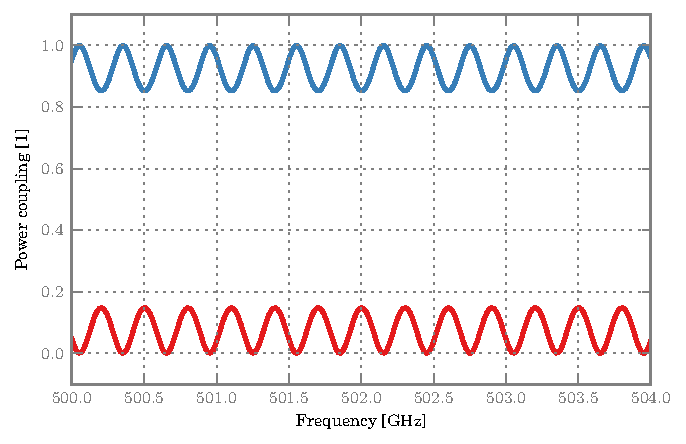
\includegraphics{simple_cavity_direct}
    \caption{Simple cavity, model result.}
    \caption*{
        The blue curve, on top, corresponds to the power coupling of port~6,
        that is the transmission through the cavity.
        The red curve, on the bottom, corresponds to the power coupling of port~1,
        that is the reflection on the cavity.
    }
    \label{fig:simple_cavity_direct}
\end{figure}
\begin{figure}[hbtp]
    \centering
    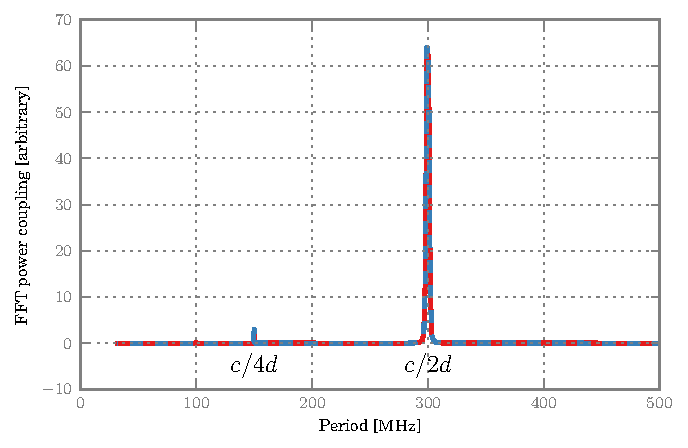
\includegraphics{simple_cavity_fft}
    \caption{Simple cavity, Fourier transform of the model result.}
    \caption*{
        The transmitted (blue) and reflected (red) wave show the same amount of modulation
        introduced by the cavity.
        The fundamental is at a period $F=c/2d$ with $c$ the speed of light in the cavity
        and $d$ the length of the cavity.
        An harmonic shows at $F=c/4d$,
        proving that the modulation is not perfectly sinusoidal.
        This spectrum was obtained by running the model for 4001 frequencies
        over a~\SI{64}{\giga\hertz} range,
        multiplying the result by a hanning window and taking a fast Fourier transform.
    }
    \label{fig:simple_cavity_fft}
\end{figure}

\Cref{fig:simple_cavity_direct} presents the result of the model for the following parameters:
\begin{itemize}
    \item refractive index $n_1=1.5$,
    \item refractive index $n_2=1.0$,
    \item distance between the interfaces $d=\SI{0.5}{\meter}$,
    \item frequency $f$ from \SIrange{500}{504}{\giga\hertz}.
\end{itemize}
The scattering matrices of the interfaces are derived from~\vref{eq:s_interface_normal} using $n_1$ and $n_2$.
The scattering matrix of the space between the interfaces is derived from~\vref{eq:scattering_distance} using $d$, $n_1$ and $f$.



%-----------------------------------------------------------------------------

\subsubsection{Periodicity}
According to \cref{eq:cavity_period}, we expect a periodicity of $F=c/2d$ where $c=c_0/n$ is the speed of light in the cavity and $d$ the length of the cavity.
With $c_0\approx \SI{2.998e8}{\meter\per\second}$, $n=1$ and $d=\SI{0.5}{\meter}$, we get $F \approx \SI{299.8}{\mega\hertz}$.

Our model agrees with our expectation, as shown by the fourrier transform in \cref{fig:simple_cavity_fft}.



%-----------------------------------------------------------------------------

\subsubsection{Energy conservation}
Examination of the results displayed in \cref{fig:simple_cavity_direct} reveals that energy is neither created nor destroyed.
The power is always positive, and the sum of the transmitted (blue) and reflected (red) power always equal 1 within numerical noise.
The power that is not transmitted through the cavity is reflected back to the source.



%=============================================================================

\subsection{Thin film beam splitter}

A thin dielectric film can be used as a beam splitter, as illustrated in \cref{fig:beam_splitter_principle}.
\begin{figure}[hbtp]
    \centering
    \input{beam_splitter_principle.pdf_tex}
    \caption{Beam splitter, principle.}
    \label{fig:beam_splitter_principle}
\end{figure}

This setup is one of the simplest way to inject local oscillator (LO) and sky signal together on a mixer.
What we have here is a heterodyne telescope.
The very transparent thin film couples most of the sky signal to the mixer, while coupling almost none of the local oscillator noise.
Unfortunately, the thin film is also transparent to the LO signal (narrow line at the LO frequency) required to pump the mixer, so the LO signal must be very strong.
This design wastes most of the LO power but has the advantage of being simple.
HIFI uses a similar approach for its bands 1, 2 and 3 (with wire grid polarizers instead of thin films though).

%-----------------------------------------------------------------------------

\subsubsection{Modeling the networks}

We can model the thin film using the principle described in \cref{sec:thin_film_at_oblique_incidence}.
Let us model a thin film of biaxially-oriented polyethylene terephthalate or ``boPET'', more commonly known under trade-mame ``Mylar''.
The table entry for ``PETP'' in the article of \citeauthor{lamb1996miscellaneous}~\cite{lamb1996miscellaneous} suggests that we choose 1.83 for the refractive index of the film at~\SI{500}{\giga\hertz}.
Using the notations of the article,
this 1.83 corresponds to the real part~$n$ of the refractive index~$\hat{n}=n-ik$.
The imaginary part~$k$ is given by the ``$\tan \delta$'' column of the table and
the equation (6) of that article, which links $\tan \delta$ to $k$: $\tan \delta = 2k/n$.
Therefore, $k = (n \tan \delta) / 2$.
With $n=1.83$ and $\tan \delta = 0.020$, we have $k=0.018$.
Our own conventions (deriving from~\cref{eq:e_z_t_real_minus}) require a sign flip: as explained in \vref{sec:polar_complex_notation}, a positive imaginary part creates absorption.
The complex refractive index of our thin film is $1.83+0.018i$.

% I know that the imaginary part of the refractive index corresponds to an absorption/gain.  The plus or minus sign probably depends on the convention chosen for k and omega.
% I have
% E = E_0 exp(ikz)
% k = \tau / \lambda
% \lambda = c / f
% c = c_0 / n
% k = \tau f n / c_0 = K n
% n = nr + i ni
% exp(iKnz) = exp(i K nr z - K ni z) = exp(iKnrz) exp(-Kniz)
% The greater ni, the stronger the attenuation.
% Therefore, I must keep ni positive.

To model the local oscillator and the mixer, I use networks that reflect \SI{10}{\percent} and transmit \SI{90}{\percent} of the incoming signal.
This is a very simplified model for a mixer or a local oscillator, but it does take into account their principle characteristic from a standing wave point of view: they reflect.

The two absorbers do not need any modeling: it is sufficient to leave the two corresponding ports of the thin film open.

%-----------------------------------------------------------------------------

\subsubsection{Simulation}
\begin{figure}[hbtp]
    \centering
    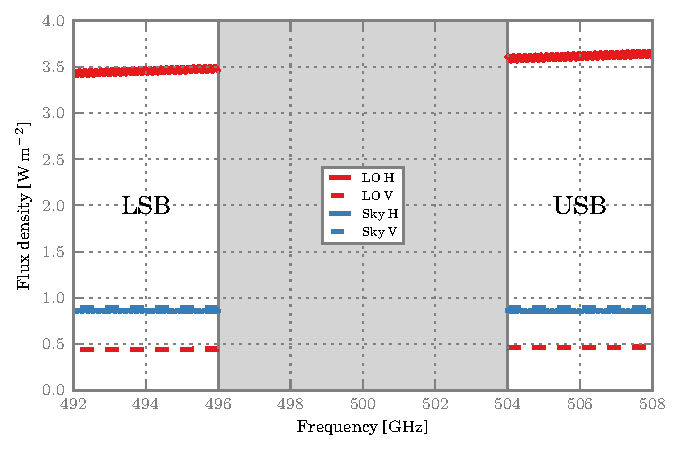
\includegraphics{thin_film_beam_splitter_detailed}
    \caption{Thin film beam splitter, detailed.}
    \label{fig:thin_film_beam_splitter_detailed}
\end{figure}
In the lower and upper side bands, the mixer receives power from two sources: the astronomical signal from the sky and the noise of the local oscillator.
In the case of HIFI, the local oscillator noise is typically two orders of magnitude stronger than the astronomical signal.
We arbitrarily set the power density from the sky at \SI{1}{\watt\per\meter\squared} and that of the local oscillator to \SI{100}{\watt\per\meter\squared}.
Since these two sources are not phase locked, we solve the system for each of them independantly.
The result is given on \cref{fig:thin_film_beam_splitter_detailed}.

We notice that the power of both the local oscillator signal and the sky signal have the same order of magnitude when hitting the mixer.
This is due to the fact that the thin film is mostly transparent, hardly reflective.
Because the sky is seen in transmission, its power is still very close to its emitted value of \SI{1}{\watt\per\meter\squared}, we couple most of the sky.
And because the local oscillator is seen in reflection, we couple only a small fraction of it (\SI{0.5}{\percent} or \SI{3.5}{\percent} depending on the polarization).
This increases the signal-to-noise ratio to an acceptable level.

The figure also illustrates that this beam splitter transmits V more than it transmits H.
As a result, V shows more sky power and less LO power.
It is in the interest of the astronomer to reject the horizontal polarization.
This can be done with a wire-grid polarizer or by using rectangular horns.

When examined closely, the H curves show some fast oscillations.
The V curves are also affected, as the next figure will show.
These oscillations are due to the cavity formed by the mixer and the local oscillator.
That cavity consists of $d=\SI{1}{\meter}$ or vacuum, which results in a period of $c_0 / 2d \approx \SI{150}{MHz}$.

The red curves show a slope.
The higher the frequency, the more LO power the mixer sees.
This slope is actually a portion of a very slow standing wave pattern.
It corresponds to the cavity formed by the two interfaces of the thin film itself.
With a speed of light of $c_0 / 1.83$ and a thickness of \SI{10}{\micro\meter}, we expect a standing wave pattern with a period of about \SI{8}{\tera\hertz}.
Calculating the real period involves knowing the pathlength of the beam inside the film, which requires some trigonometry, but the order remains at several terahertz.

In a real system, we would not have access to all the details of \cref{fig:thin_film_beam_splitter_detailed}.
Indeed, for a given frequency, we receive the sum of the LO and sky power without being able to tell them apart.
Furthermore, mixers fold spectra, which adds the lower and upper side bands together.
Finally, the polarizations become undistinguishable.
In \cref{fig:thin_film_beam_splitter_folded}, we have summed the two sources and folded the spectra; however we kept the polarization intact.
These summations were done in power and not in field, because the LSB, USB, LO and sky power are not phase locked to each other: each signal is coherent with itself only, not with the others.

\begin{figure}[hbtp]
    \centering
    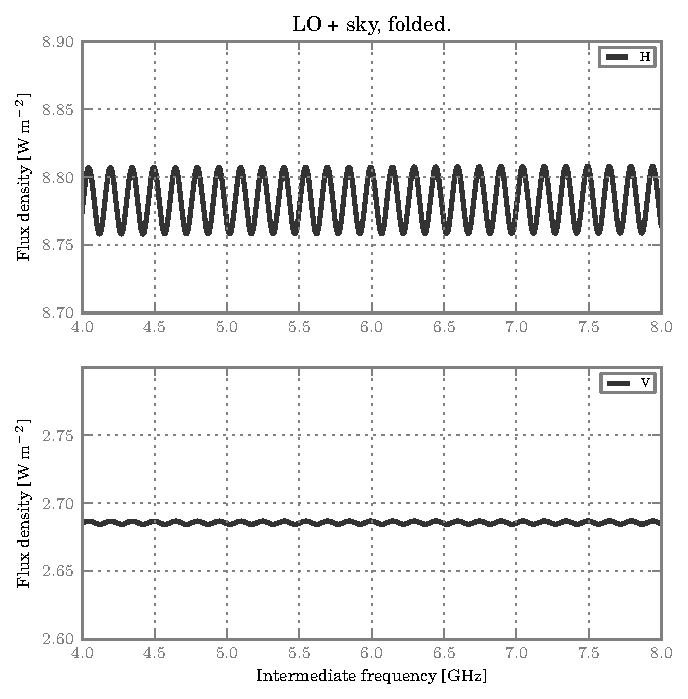
\includegraphics{thin_film_beam_splitter_folded}
    \caption{Thin film beam splitter, folded.}
    \label{fig:thin_film_beam_splitter_folded}
\end{figure}

The slope due to the cavity inside the thin film seems to have disappeared.
This is expected: the lower sideband is flipped before being added to the upper sideband.
Therefore, when the slope goes up for one, it goes down for the other,
and they compensate quite well.
Some other values for the LO frequency or film thickness can allow the thin film cavity to leave a more obvious signature on the folded spectrum.

This figure reveals that the V polarization is also affected by standing wave, as we mentionned earlier.
It is much weaker in V than in H because the thin film is more transparent for V.
This means that the V-polarized light is more likely to exit the cavity either toward the sky or toward the open port on the right, both perfect aborbers.
This standing wave pattern has a period of \SI{150}{\mega\hertz}, which is expected of the LO--mixer cavity.

\subsubsection{Sideband ratio}
Standing waves change the coupling of the mixer to the signal.
This coupling is a priori different in the lower and upper sideband.
Therefore, each channel of a folded spectrum is a priori imbalanced, giving more weight to either sideband.

In the HIFI consortium, we agreed on the following definition~\eqref{eq:sideband_ratio} of the sideband ratio as a metric for the imbalance between the two sidebands.
A perfectly balanced system has a sideband ratio of 0.5.
If the sideband ratio is greater than 0.5, then the channel is USB-dominated.
If it is lower than 0.5, the channel is LSB-dominated.
\begin{equation}
    \text{sideband ratio} =
    \frac{
        \text{USB power coupling}
    }{
        \text{LSB power coupling} + \text{USB power coupling}
    }
    \label{eq:sideband_ratio}
\end{equation}

\begin{figure}[hbtp]
    \centering
    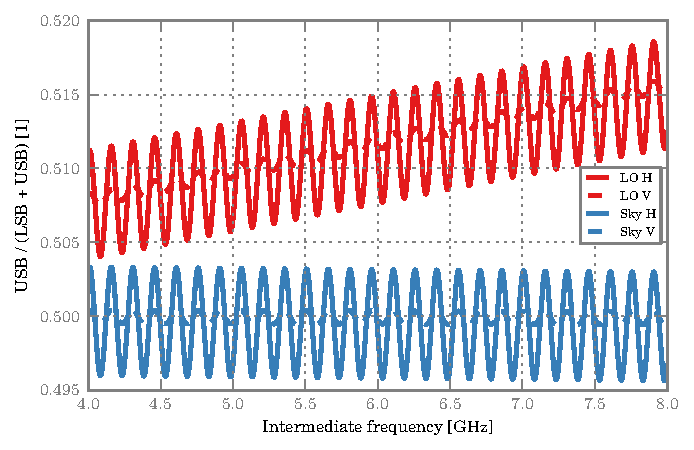
\includegraphics{thin_film_beam_splitter_sbr}
    \caption{Thin film beam splitter, sideband ratio.}
    \label{fig:thin_film_beam_splitter_sbr}
\end{figure}
\Cref{fig:thin_film_beam_splitter_sbr} shows the sideband ratio for the LO and the sky for both polarizations.
The slope comes from very slow modulation due to the cavity inside the thin film.
Note that it is clearly visible here, even on the sky, while it was hardly noticeable on the folded spectrum of \cref{fig:thin_film_beam_splitter_folded}.
A flat continuum does not guarantee a flat sideband ratio.

With this system, the standard deviation of the sideband ratio for is \SI{2.6}{\percent} for H and \SI{0.3}{\percent} for V.
This is the error that we can expect when measuring a thin emission line on a perfectly flat continuum after an infinitely long integration time: the line can fall anywhere between a peak and a crest of this standing wave pattern.

\subsubsection{The many LO--mixer cavities}

\Cref{fig:thin_film_beam_splitter_folded_fft} shows
the fast Fourier Transform of \cref{fig:thin_film_beam_splitter_folded} (using a Hanning window).
It peaks at the expected~\SI{150}{\mega\hertz} and shows a very weak harmonic at~\SI{75}{\mega\hertz}.
The harmonics are very weak because the cavity is of very low quality: the film is very transparent and the light leaves the cavity quickly.

\begin{figure}[hbtp]
    \centering
    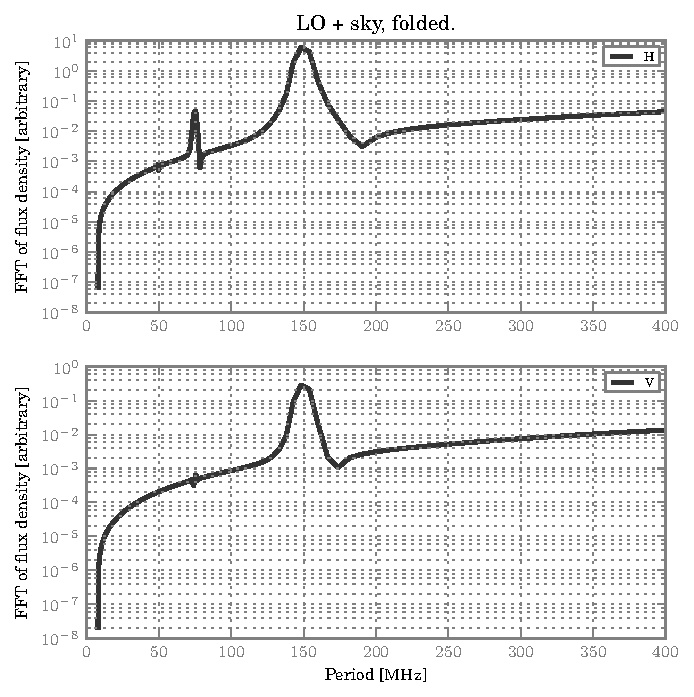
\includegraphics{thin_film_beam_splitter_folded_fft}
    \caption{Thin film beam splitter, folded, FFT.}
    \label{fig:thin_film_beam_splitter_folded_fft}
\end{figure}

The astute reader may be wondering why we are observing only two cavities (LO--mixer and inside thin film) instead of an infinity.
Indeed, there is no such thing as \textit{the} LO--mixer cavity, there are an infinity of them.
The shortest one is the one corresponding to a single reflection on the near side of the thin film.
Then, another possible path involves entering the thin film, being reflected by the far side, traversing the film again, and being transmitted toward the detector.
A third path involves two round-trips inside the film, and a fourth path involves three round-trips, etc.
Why don't these many cavities show up as as many peaks on the FFT?
The answer is simple: our FFT does not have enough resolution.

Our bandpass $B$ of \SI{4}{\giga\hertz} does not allow to resolve a variation of \SI{10}{\micro\meter} in a cavity.
$B = c / 2d$ with $d=\SI{10}{\micro\meter}$ and $c=c_0$ yields $B \approx \SI{15}{\tera\hertz}$, which is way beyond our \SI{4}{\giga\hertz}.
If we reverse the calculation, $d=c/2B$ for $B=\SI{4}{\giga\hertz}$ gives $d \approx \SI{37}{mm}$: our FFT can distinguish cavities that differ by more than \SI{4}{\centi\meter}.
This limitation affects only the FFT as a tool used for visualizing our data; our model has no such limitation.

\begin{figure}[hbtp]
    \centering
    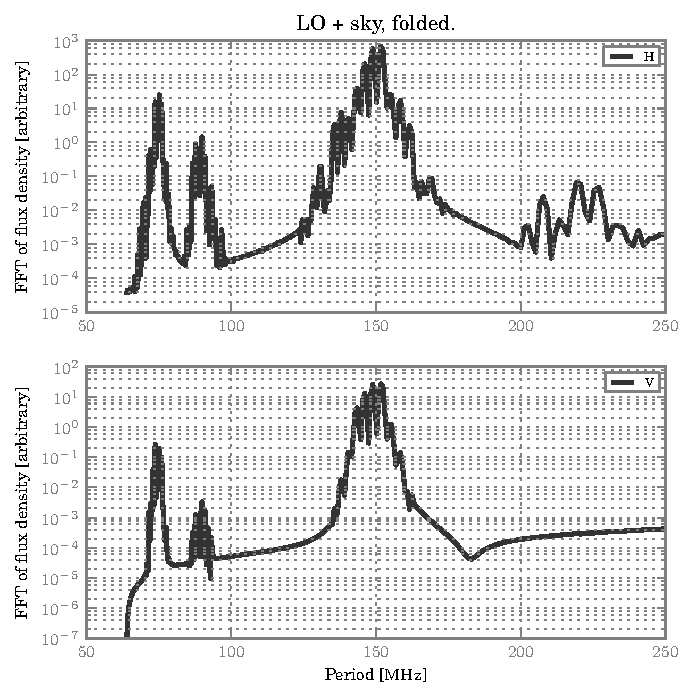
\includegraphics{thin_film_beam_splitter_folded_fft_hr}
    \caption{Thin film beam splitter, folded, FFT, high resolution.}
    \label{fig:thin_film_beam_splitter_folded_fft_hr}
\end{figure}
\Cref{fig:thin_film_beam_splitter_folded_fft_hr} shows the FFT of the same system for a bandwidth of~\SI{32}{\giga\hertz}, a film thickness of~\SI{1}{\centi\meter}, and no imaginary part in the refractive index of the mylar (otherwise the absorption would hide the result).
Once the system is modified to meet the expectations of the FFT, then the FFT does show the expected many peaks around~\SI{150}{\mega\hertz}, which prove that our model takes into account the infinity of LO--mixer cavities.
